\RequirePackage[l2tabu,orthodox]{nag}

% TODO: decide if one-sided/two-sided
%\documentclass[headsepline,footsepline,footinclude=false,fontsize=11pt,paper=a4,listof=totoc,bibliography=totoc,BCOR=12mm,DIV=12]{scrbook} % two-sided % original source stated: BCOR=12mm,DIV=12
\documentclass[headsepline,footsepline,footinclude=false,oneside,fontsize=11pt,paper=a4,listof=totoc,bibliography=totoc,DIV=12]{scrbook} % one-sided

% TODO: change citation style in settings
\PassOptionsToPackage{table,svgnames,dvipsnames}{xcolor}

\usepackage[utf8]{inputenc}
\usepackage[T1]{fontenc}
\usepackage[sc]{mathpazo}
\usepackage[ngerman,english]{babel} % english is the same as american or USenglish
\usepackage[autostyle]{csquotes}
\usepackage{textcomp}
\usepackage{float}
\usepackage[%
  backend=biber,
  url=true,
  style=numeric, % alphabetic, numeric
  sorting=none, % default == nty, https://tex.stackexchange.com/questions/51434/biblatex-citation-order
  maxnames=4,
  minnames=3,
  maxbibnames=99,
  giveninits,
  uniquename=init]{biblatex} % TODO: adapt citation style
\usepackage{graphicx}
\usepackage{scrhack} % necessary for listings package
\usepackage{listings}
\usepackage{lstautogobble}
\usepackage{tikz}
\usepackage{pgfplots}
\usepackage{pgfplotstable}
\usepackage{booktabs} % for better looking table creations, but bad with vertical lines by design (package creator despises vertical lines)
\usepackage[final]{microtype}
\usepackage{caption}
\usepackage[hidelinks]{hyperref} % hidelinks removes colored boxes around references and links
\usepackage{ifthen} % for comparison of the current language and changing of the thesis layout
\usepackage{pdftexcmds} % string compare to work with all engines
\usepackage{paralist} % for condensed enumerations or lists
\usepackage{subfig} % for having figures side by side
\usepackage{siunitx} % for physical accurate units and other numerical presentations
\usepackage{multirow} % makes it possible to have bigger cells over multiple rows in a table
\usepackage{array} % different options for table cell orientation
\usepackage{makecell} % allows nice manual configuration of cells with linebreaks in \thead and \makecell with alignments
\usepackage{pdfpages} % for including multiple pages of pdfs
\usepackage{adjustbox} % can center content wider than the \textwidth
\usepackage{tablefootnote} % for footnotes in tables as \tablefootnote
\usepackage{threeparttable} % another way to add footnotes as \tablenotes with \item [x] <your footnote> after setting \tnote{x} 
\usepackage{wrapfig}
\usepackage[colorinlistoftodos,prependcaption]{todonotes}

% https://tex.stackexchange.com/questions/42619/x-mark-to-match-checkmark
\usepackage{amssymb}% http://ctan.org/pkg/amssymb
\usepackage{pifont}% http://ctan.org/pkg/pifont
\newcommand{\cmark}{\ding{51}}%
\newcommand{\xmark}{\ding{55}}%


\usepackage[acronym,xindy,toc]{glossaries} % TODO: include "acronym" if glossary and acronym should be separated
\makeglossaries
\loadglsentries{pages/glossary.tex} % important update for glossaries, before document


\bibliography{bibliography}

\setkomafont{disposition}{\normalfont\bfseries} % use serif font for headings
\linespread{1.05} % adjust line spread for mathpazo font

% Add table of contents to PDF bookmarks
\BeforeTOCHead[toc]{{\cleardoublepage\pdfbookmark[0]{\contentsname}{toc}}}

% Define TUM corporate design colors
% Taken from http://portal.mytum.de/corporatedesign/index_print/vorlagen/index_farben
\definecolor{TUMBlue}{HTML}{0065BD}
\definecolor{TUMSecondaryBlue}{HTML}{005293}
\definecolor{TUMSecondaryBlue2}{HTML}{003359}
\definecolor{TUMBlack}{HTML}{000000}
\definecolor{TUMWhite}{HTML}{FFFFFF}
\definecolor{TUMDarkGray}{HTML}{333333}
\definecolor{TUMGray}{HTML}{808080}
\definecolor{TUMLightGray}{HTML}{CCCCC6}
\definecolor{TUMAccentGray}{HTML}{DAD7CB}
\definecolor{TUMAccentOrange}{HTML}{E37222}
\definecolor{TUMAccentGreen}{HTML}{A2AD00}
\definecolor{TUMAccentLightBlue}{HTML}{98C6EA}
\definecolor{TUMAccentBlue}{HTML}{64A0C8}

% Settings for pgfplots
\pgfplotsset{compat=newest}
\pgfplotsset{
  % For available color names, see http://www.latextemplates.com/svgnames-colors
  cycle list={TUMBlue\\TUMAccentOrange\\TUMAccentGreen\\TUMSecondaryBlue2\\TUMDarkGray\\},
}

% Settings for lstlistings

% Use this for basic highlighting
\lstset{%
  basicstyle=\ttfamily,
  columns=fullflexible,
  autogobble,
  keywordstyle=\bfseries\color{TUMBlue},
  stringstyle=\color{TUMAccentGreen}
}

% use this for C# highlighting
% %\setmonofont{Consolas} %to be used with XeLaTeX or LuaLaTeX
% \definecolor{bluekeywords}{rgb}{0,0,1}
% \definecolor{greencomments}{rgb}{0,0.5,0}
% \definecolor{redstrings}{rgb}{0.64,0.08,0.08}
% \definecolor{xmlcomments}{rgb}{0.5,0.5,0.5}
% \definecolor{types}{rgb}{0.17,0.57,0.68}

% \lstset{language=[Sharp]C,
% captionpos=b,
% %numbers=left, % numbering
% %numberstyle=\tiny, % small row numbers
% frame=lines, % above and underneath of listings is a line
% showspaces=false,
% showtabs=false,
% breaklines=true,
% showstringspaces=false,
% breakatwhitespace=true,
% escapeinside={(*@}{@*)},
% commentstyle=\color{greencomments},
% morekeywords={partial, var, value, get, set},
% keywordstyle=\color{bluekeywords},
% stringstyle=\color{redstrings},
% basicstyle=\ttfamily\small,
% }

% Settings for search order of pictures
\graphicspath{
    {logos/}
    {figures/}
}

% Set up hyphenation rules for the language package when mistakes happen
\babelhyphenation[english]{
an-oth-er
ex-am-ple
}

% Decide between
%\newcommand{\todo}[1]{\textbf{\textsc{\textcolor{TUMAccentOrange}{(TODO: #1)}}}} % for one paragraph, otherwise error!
%\newcommand{\done}[1]{\textit{\textsc{\textcolor{TUMAccentBlue}{(Done: #1)}}}} % for one paragraph, otherwise error!
% and
%\newcommand{\todo}[1]{{\bfseries{\scshape{\color{TUMAccentOrange}[(TODO: #1)]}}}} % for multiple paragraphs
\newcommand{\done}[1]{{\itshape{\scshape{\color{TUMAccentBlue}[(Done: #1)]}}}} % for multiple paragraphs
% for error handling of intended behavior in your latex documents.

\newcommand{\tabitem}{~~\llap{\textbullet}~~}

\newcolumntype{P}[1]{>{\centering\arraybackslash}p{#1}} % for horizontal alignment with limited column width
\newcolumntype{M}[1]{>{\centering\arraybackslash}m{#1}} % for horizontal and vertical alignment with limited column width
\newcolumntype{L}[1]{>{\raggedright\arraybackslash}m{#1}} % for vertical alignment left with limited column width
\newcolumntype{R}[1]{>{\raggedleft\arraybackslash}m{#1}} % for vertical alignment right with limited column width

% TODO: change thesis information
\newcommand*{\getUniversity}{Technische Universität München}
\newcommand*{\getFaculty}{School of Computation, Information and Technology - Informatics}
\newcommand*{\getTitle}{Deep Learning Based Analysis of Tumor-infiltrating Lymphocytes in H\&E Stained Histological Sections for Survival Prediction of Breast Cancer patients}
\newcommand*{\getTitleGer}{Deep Learning basierte Analyse von tumorinfiltrierenden Lymphozyten in H\&E gefärbten histologischen Schnitten zur Überlebensvorhersage von Brustkrebspatienten}
\newcommand*{\getAuthor}{Margaryta Olenchuk}
\newcommand*{\getDoctype}{Master's Thesis in Biomedical Computing}
\newcommand*{\getSupervisor}{Prof. Dr. Peter Schüffler}
\newcommand*{\getAdvisor}{Dr. Philipp Wortmann, Ansh Kapil}
\newcommand*{\getSubmissionDate}{15.12.2022}
\newcommand*{\getSubmissionLocation}{Munich}

\begin{document}

% TODO: decide on used language
%\selectlanguage{ngerman}
\selectlanguage{english}

% Set page numbering to avoid "destination with the same identifier has been already used" warning for cover page.
% (see https://en.wikibooks.org/wiki/LaTeX/Hyperlinks#Problems_with_Links_and_Pages).
\pagenumbering{alph}
\begin{titlepage}
  % HACK for two-sided documents: ignore binding correction for cover page.
  % Adapted from Markus Kohm's KOMA-Script titlepage=firstiscover handling.
  % See http://mirrors.ctan.org/macros/latex/contrib/koma-script/scrkernel-title.dtx,
  % \maketitle macro.
  \oddsidemargin=\evensidemargin\relax
  \textwidth=\dimexpr\paperwidth-2\evensidemargin-2in\relax
  \hsize=\textwidth\relax

  \centering

  \IfFileExists{logos/tum.pdf}{%
    
\includegraphics[height=20mm]{logos/tum.pdf}
  }{%
    \vspace*{20mm}
  }

  \vspace{5mm}
  {\Large\MakeUppercase{\getFaculty{}}}\\

  \vspace{5mm}
  {\large\MakeUppercase{\getUniversity{}}}\\

  \vspace{20mm}
  {\Large \getDoctype{}}

  \vspace{15mm}
  \makeatletter
  \ifthenelse{\pdf@strcmp{\languagename}{english}=0}
  {\huge\bfseries \getTitle{}}
  {\huge\bfseries \getTitleGer{}}
  \makeatother

  \vspace{15mm}
  {\LARGE \getAuthor{}}

  \IfFileExists{logos/faculty.png}{%
    \vfill{}
    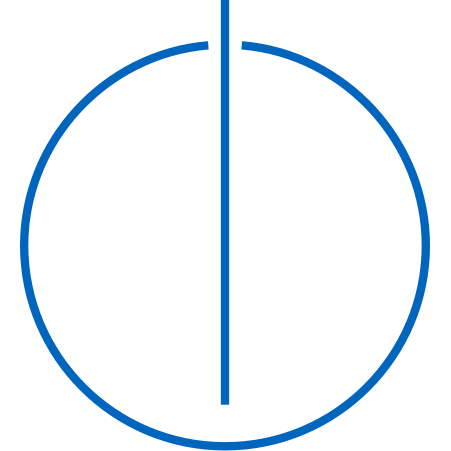
\includegraphics[height=20mm]{logos/faculty.png}
  }{}
\end{titlepage}


\frontmatter{}

\begin{titlepage}
  \centering

  \IfFileExists{logos/tum.pdf}{%
    
\includegraphics[height=20mm]{logos/tum.pdf}
  }{%
    \vspace*{20mm}
  }

  \vspace{5mm}
  {\Large\MakeUppercase{\getFaculty{}}}\\

  \vspace{5mm}
  {\large\MakeUppercase{\getUniversity{}}}\\

  \vspace{20mm}
  {\Large \getDoctype{}}

  \makeatletter
  \vspace{15mm}
  \ifthenelse{\pdf@strcmp{\languagename}{english}=0}
  {
  {\huge\bfseries \getTitle{}}

  \vspace{10mm}
  {\huge\bfseries \foreignlanguage{ngerman}{\getTitleGer{}}}
  }
  {
  {\huge\bfseries \getTitleGer{}}

  \vspace{10mm}
  {\huge\bfseries \foreignlanguage{english}{\getTitle{}}}
  }
  \makeatother

  \vspace{15mm}
  \begin{tabular}{l l}
    Author:          & \getAuthor{} \\
    Supervisor:      & \getSupervisor{} \\
    Advisor:         & \getAdvisor{} \\
    Submission Date: & \getSubmissionDate{} \\
  \end{tabular}

\end{titlepage}

\cleardoublepage{}

\thispagestyle{empty}
\vspace*{0.8\textheight}
\noindent
\makeatletter
\ifthenelse{\pdf@strcmp{\languagename}{english}=0}
{I confirm that this \MakeLowercase{\getDoctype{}} is my own work and I have documented all sources and material used.}
{Ich versichere, dass ich diese \getDoctype{} selbstständig verfasst und nur die angegebenen Quellen und Hilfsmittel verwendet habe.}
\makeatother

\vspace{15mm}
\noindent
\getSubmissionLocation{}, \getSubmissionDate{} \hspace{50mm} \getAuthor{}

\cleardoublepage{}

\makeatletter
\ifthenelse{\pdf@strcmp{\languagename}{english}=0}
{\addcontentsline{toc}{chapter}{Acknowledgments}}
{\addcontentsline{toc}{chapter}{Danksagungen}}
\makeatother
\thispagestyle{empty}

\vspace*{20mm}

\begin{center}
\makeatletter
\ifthenelse{\pdf@strcmp{\languagename}{english}=0}
{\usekomafont{section} Acknowledgments}
{\usekomafont{section} Danksagungen}
\makeatother
\end{center}

\vspace{10mm}

I would like to say thanks to all who supported me in the last few months, to all who endured my mood, and to all, who encouraged me to stay motivated. Thank you!

I would like to take this opportunity to thank my advisor Peter Schüffler for giving me the opportunity to write my thesis at his chair, allowing me to explore my topic to the fullest, and taking time for numerous meetings and detailed discussions. Thank you and hope we will meet in person someday.

Special thanks also go to all Munich AstraZeneca members for providing amazing resources and constant support along the way. Many thanks to my advisors, Philipp Wortmann and Ansh Kapil for trusting me to work on a remarkable topic. I have learned a lot, thanks to you and your guidance. Particular thanks go to Armin Meier who always found time to discuss frustrating details and provided elegant solutions every time. And thanks to all other sync meetings and lunch break discussions with Guillaume Potdevin, Abdullah Hayran, Gordan Prastalo, Bianca Mocanu, and Srividhya Sathya Narayanan. 

Finally, I would like to say thanks for all the non-scientific support. To my family, especially my parents and my grandmother, who repeatedly reminded me not to work too hard.
Ukrainian Armed Forces and all defenders and volunteers for protection and the chance to do science. To all Ukrainians for sharing these difficult times with me and reminding me that there should still be room for normal even in war times.  And thanks to my wonderful friends Lena Shevtsova and Laczik sisters, Dalma and Dori for being there for me.

Thank you.

\cleardoublepage{}
 % TODO: if you don't have anyone to thank for or don't wish to publish it, comment this line out.
\chapter{\abstractname}

Breast cancer is the most common type of cancer worldwide with a high mortality rate causing millions of cancer-related deaths annually.
Optimization of diagnostic biomarkers is essential to improve breast cancer prognosis and therapeutic outcomes.
According to the International Immuno-Oncology Biomarker Working Group, early-stage disease clinicopathological risk stratification is currently performed using a limited set of features such as tumor size and lymph node status, that do not stratify patients with sufficient granularity to permit selection for clinical trials. 
%The results of high-throughput technology analysis have identified transcriptomic or proteomic features which are associated with particular histological features. 
%Hence, the histological appearance of a tumor represents a useful cancer phenotype that can be further explored, and contribute to staging and stratification.

The quantification of mononuclear immune cells that infiltrate tumor tissue, named tumor-infiltrating lymphocytes (TILs) is a clinically useful biomarker for breast cancer progression.
TILs in tumors and the surrounding microenvironment are thought to reflect the ongoing anti-tumor immune response of the host.
TIL analysis is typically performed by pathologists that manually estimate the proportion of TILs in a histological appearance.

The automatic assessment of TILs by computational image analysis is valuable for standardization and potential use in a clinical setting.
This thesis shows that TIL evaluation can be automated with deep learning-based techniques. The developed pipeline segments tissue relevant for TIL score, such as stromal and tumorous regions using DeepLabv3+, and detects TILs based on the publicly released TiGER challenge data containing digital pathology images of Her2 positive and Triple Negative breast cancer whole-slide images.
The tissue segmentation model scored 0.85 Dice score on the test set and TIL detection was approached as segmentation with a transformer-based architecture - SegFormer, which is novel for computational pathology, and scored 0.66 F1-score on the test set.

The application of deep learning approaches permitted the discovery of image-based features that would be demanding to identify per hand, particularly if they only exist in small groups of patients. It made it feasible not only to show the effect of TIL density in stroma but experiment with various borders of stroma, tumor-associated stroma, and tumor, as well as novel heterogeneity features.
Applied to TCGA-BRCA clinical data, TIL features demonstrated their ability to successfully stratify the patients into groups of high and low TIL density. In Cox proportional hazards model TIL density in tumor associated stroma border of 100 \textmu m achieved concordance of 0.59, p-value 0.00018, and 0.78 hazard ratio, supporting the assumption that the high level of TILs plays a role in prolonged survival probability and therefore can be used as a prognostic marker for breast cancer patients.


\makeatletter
\ifthenelse{\pdf@strcmp{\languagename}{english}=0}
{\renewcommand{\abstractname}{Kurzfassung}}
{\renewcommand{\abstractname}{Abstract}}
\makeatother

\chapter{\abstractname}

%TODO: Abstract in other language
\begin{otherlanguage}{ngerman} 
Brustkrebs ist weltweit die häufigste Krebsart mit einer hohen Sterblichkeitsrate, die jährlich Millionen von krebsbedingten Todesfällen verursacht.
Die Optimierung diagnostischer Biomarker ist für die Verbesserung der Brustkrebsprognose und der therapeutischen Ergebnisse von essenzieller Bedeutung.
Nach Angaben der International Immuno-Oncology Biomarker Working Group erfolgt die klinisch-pathologische Risikostratifizierung im Frühstadium der Erkrankung derzeit anhand einer begrenzten Anzahl von Merkmalen wie Tumorgröße und Lymphknotenstatus, die die Patienten nicht ausreichend genau einteilen, um eine Auswahl für klinische Studien zu ermöglichen. 

Die Quantifizierung von mononukleären Immunzellen, die in das Tumorgewebe eindringen und als tumorinfiltrierende Lymphozyten (TILs) bezeichnet werden, ist ein klinisch nützlicher Biomarker für das Fortschreiten von Brustkrebs.
Es wird angenommen, dass TILs in Tumoren und der umgebenden Mikroumgebung die laufende Anti-Tumor-Immunreaktion des Wirts widerspiegeln.
Die TIL-Analyse wird in der Regel von Pathologen durchgeführt, die den Anteil der TILs in einem histologischen Befund manuell schätzen.

Die automatische Bewertung von TILs durch computergestützte Bildanalyse ist wertvoll für die Standardisierung und den potenziellen Einsatz in einem klinischen Umfeld.
Diese Arbeit zeigt, dass die TIL-Bewertung mit Deep-Learning-basierten Techniken automatisiert werden kann. Die entwickelte Pipeline segmentiert Gewebe, das für die TIL-Bewertung relevant ist, wie z. B. stromale und tumoröse Regionen unter Verwendung von DeepLabv3+, und erkennt TILs auf der Grundlage der öffentlich veröffentlichten TiGER-Challenge-Daten, die digitale Pathologiebilder von Her2-positiven und dreifach negativen Brustkrebs-Ganzbildaufnahmen enthalten.
Das Gewebesegmentierungsmodell erzielte 0,85 Dice-Wert in der Testreihe und die TIL-Erkennung wurde als Segmentierung mit einer transformatorbasierten Architektur - SegFormer - angegangen, die für die computergestützte Pathologie neu ist und 0,66 F1-Wert in der Testreihe erzielte.

Die Anwendung von Deep-Learning-Ansätzen ermöglichte die Entdeckung von bildbasierten Merkmalen, die per Hand nur schwer zu identifizieren wären, insbesondere wenn sie nur bei kleinen Patientengruppen vorkommen. Dadurch konnte nicht nur die Auswirkung der TIL-Dichte im Stroma aufgezeigt, sondern auch mit verschiedenen Grenzen des Stromas, tumorassoziierten Stromas und Tumors sowie mit neuen Heterogenitätsmerkmalen experimentiert werden.
Bei der Anwendung auf die klinischen Daten des TCGA-BRCA zeigten die TIL-Merkmale ihre Fähigkeit, die Patienten erfolgreich in Gruppen mit hoher und niedriger TIL-Dichte zu stratifizieren. Im Cox-Proportional-Hazards-Modell erreichte die TIL-Dichte in der tumorassoziierten Stromagrenze von 100 \textmu m eine Übereinstimmung von 0,59, einen p-Wert von 0,00018 und eine Hazard Ratio von 0,78, was die Annahme stützt, dass die hohe TIL-Dichte eine Rolle bei der verlängerten Überlebenswahrscheinlichkeit spielt und daher als prognostischer Marker für Brustkrebspatientinnen verwendet werden kann.
\end{otherlanguage}


% Undo the name switch
\makeatletter
\ifthenelse{\pdf@strcmp{\languagename}{english}=0}
{\renewcommand{\abstractname}{Abstract}}
{\renewcommand{\abstractname}{Kurzfassung}}
\makeatother
\microtypesetup{protrusion=false}
\tableofcontents{}
\microtypesetup{protrusion=true}

\mainmatter{}


\chapter{Introduction}\label{chapter:introduction}
%Breast cancer bad 
Breast cancer is the most common form of cancer diagnosed worldwide
and the leading cause of cancer-related death among women.~\cite{chhikara2022global}
It is a heterogeneous disease, consisting of several morphological and molecular subtypes.
The molecular subtypes are among the most important factors to characterize
breast cancer. Four main groups are defined
based on the status of several receptors used in clinical practice~\cite{home},
namely the Hormonal Receptor (HR, which is positive if either Estrogen Receptor (ER) or Progesterone Receptor (PR) are positive)
and of their human epidermal growth factor receptor 2 (Her2):
\begin{enumerate}
    \itemsep0em 
    \item Luminal A (HR positive, Her2 negative)
    \item Luminal B (HR positive, Her2 positive)
    \item Her2 enriched (HR negative, Her2 positive) 
    \item Triple Negative (HR negative, Her2 negative)
\end{enumerate}
Regardless of the subtype, for diagnostic confirmation of breast cancer
a patient’s tissue sample is sectioned
onto microscope slides for staining, often with hematoxylin and eosin (H\&E), followed by
a visual diagnosis by a pathologist. Pathologists examine a tissue specimen
for abnormalities that indicate breast cancer. 
Since cancer causes changes in tissue at the sub-cellular scale, an analysis of normal and tumor tissue can provide novel insights into
tissue characteristics and can lead to a better understanding of mechanisms underlying cancer onset, progression
and provide valuable information for medical decision making such as treatment choices.~\cite{vu2019methods}
While the manual examination continues to be widely applied in clinical settings, it is a
subjective and is not scalable to translational and clinical research studies
involving a high number of high-resolution whole slide tissue images (WSIs). 
Hence, there is an increased need
for reliable and efficient automated methods to complement the traditional manual
examination of tissue samples. 
Due to advancing technology and access to a large amount of data, deep learning methods
have garnered a lot of interest in computer vision for the digital pathology domain.
The two most common computerized tasks in WSI
analysis are the segmentation of microscopic structures, structures like tumor regions and
smaller nuclei and cells, and the classification of image regions or even whole images.
And while there are a great number of deep learning based analysis pipelines in the digital pathology domain,
automated algorithms also contribute to the development and testing of reliable prognostic and predictive biomarkers
to help clinicians choose the best treatment for each patient.

The differentiation between breast cancer
types and subtypes is essential. This thesis is focused on Her2 positive
and Triple Negative breast cancer (TNBC) subtypes since they have the worst prognosis,
and therefore subject to a large corpus of research in prognostic and predictive biomarkers,
aiming at improving patient management and prognosis. TNBC is an aggressive type of cancer and
due to the lack of all three receptors, it has a limited response to hormonal and immune treatments.
Cancers of this type are known to have high recurrence rates and
poor prognoses compared to non-TN breast cancers.~\cite{cao2020triple}
There are multiple reported biomarkers for TNBC, such as epidermal growth factor receptor,
vascular endothelial growth factor, C-kit, and basal cytokeratins.~\cite{yadav2015biomarkers} Moreover, a significant
percentage of TNBCs are known to carry BRCA1 mutations,
in which tumor cells are defective in homologous recombination DNA repair mechanisms.
But this thesis focuses on the tumor-infiltrating lymphocytes (TILs), which could be examined 
from WSIs therefore directly accessible without the need for any further testing or additional data source. 

TILs are mononuclear immune cells that infiltrate tumor tissue and have been detected in almost all solid tumors,
including breast cancer.~\cite{laenkholm2022incorporation}
The development and progression of malignant tumors can be characterized by an interaction of the cells
in the tumor microenvironment and TILs.
In the early stage HER2-positive and TNBC, immune infiltrates are detectable in up to 75\% of tumors.~\cite{dieci2018update}
Accumulating evidence indicates that tumor-infiltrating lymphocytes are clinically useful biomarkers in TNBC and HER2-positive
and that they play an essential role in cancer progression.~\cite{gao2020prognostic}
The patients with a high proportion of TILs in the tumor tissue and high immunogenicity of the tumor
were shown to respond better to the chemotherapy. Further research and development of additional
TILs related biomarkers would not only grand clinicians important prognostic information but also promote the
research focus of novel treatments and therapeutics.
Analysis of TILs with exhausted phenotype is associated with loss of antitumor immunity.
Single-cell RNA-seq of TILs has been already performed to search for new immune checkpoint blockade targets that enable
the precise definition and even novel development of therapeutic strategies to overcome T-cell exhaustion.
Therapeutic approaches to influence T-cell exhaustion have been already developed to target proteins CTLA-4, PD-1, and PD-L1
and have proven to be effective in treating melanoma and non-small-cell lung cancer during ongoing trials.~\cite{postow2015immune}
TILs in TNBC patients also display immuno-suppressive phenotypes~\cite{chung2017single} and the number of TILs detected by TNBC
patients is higher than in other breast cancer subgroups~\cite{schneeweiss2019diagnosis} which makes TNBC a valid target for further
TILs sequencing research for its application in the context of TN breast cancer or in search of further targets.

The aim of this work is to experiment with computer algorithms for the automated image segmentation and tumor-infiltrating
lymphocytes assessment in Her2 positive
and Triple Negative breast cancer histopathology slides based on Tumor InfiltratinG lymphocytes in
breast cancER (TiGER) challenge. This works partly relies on publically
released TiGER challenge and TCGA dataset to also further experiment with the prognostic significance of computer-generated TILs scores
for predicting patients' survival.
\chapter{Related work}
\section{Deep learning-based semantic segmentation}
The focus of the following chapter is the deep learning-based approaches for semantic image segmentation, particularly for medical images analysis. As Shephard, Adam et al. discuss~\cite{shephard2022tiager} segmentation of tumor/stroma as well as the detection of TILs can be viewed as semantic segmentation problem. 

The goal of semantic segmentation is to assign each image pixel to a category label corresponding to the underlying object. Due to the success of deep learning models in a wide range of vision applications, various deep learning-based algorithms have been developed and published in the literature~\cite{minaee2021image}. One of the most prominent deep learning architectures used by the computer vision community include fully convolutional networks (FCNs)~\cite{long2015fully}, encoder-decoders~\cite{noh2015learning}, generative adversarial networks (GANs)~\cite{goodfellow2014generative} and recurrent neural networks (RNNs)~\cite{rumelhart1986learning}.

\subsection{Fully convolutional networks (FCNs)}
FCNs~\cite{long2015fully} are among the most widely used architectures for computer vision tasks and their general architecture consists of several learnable convolutions, pooling layers, and a final 1$\times$1 convolution. While models based on this architecture perform well on challenging segmentation benchmarks, e.g. applied on scene segmentation~\cite{yu2020context} and instance aware semantic segmentation~\cite{li2017fully}, they are also used on segmentation problems in histology domain such as colon glands segmentation~\cite{bentaieb2016topology}, identification of muscle and messy regions in contexts of inflammatory bowel disease~\cite{wang2016deep} as well as nuclei~\cite{natarajan2020segmentation} and TILs~\cite{amgad2019joint} segmentation for breast cancer all performed on the Hematoxylin and Eosin (H\&E) stained histopathology images. Moreover, the FCN method was applied for semantic segmentation of TCGA~\cite{gutman2013cancer} breast data set~\cite{amgad2019structured}, which is also used in this thesis. However, despite its popularity, the conventional FCN model has limitations such as loss of localization and the inability to process potentially useful global context information due to a series of down-sampling and a high sampling rate.

\subsection{Encoder-decoder networks}
A popular group of deep learning models for semantic image segmentation that aims to solve the aforementioned issues of FCNs is based on the convolutional encoder-decoder architecture~\cite{noh2015learning}. Their model consists of two parts, an encoder consisting of convolutional layers and a deconvolution network that consists of deconvolution and unpooling layers that take the feature vector as input and generate a map of pixel-wise class probabilities. Example for such a convolutional encoder-decoder architecture for image segmentation is SegNet~\cite{badrinarayanan2017segnet}. The SegNet's encoder network has 13 convolutional layers with corresponding layers in the decoder. The final decoder output is fed to a multi-class soft-max classifier to produce class probabilities for each pixel independently. The main feature of SegNet is that the decoder uses pooling indices computed in the max-pooling step of the corresponding encoder to perform non-linear upsampling. This allows it to achieve high scores for road scene understanding problems~\cite{badrinarayanan2017segnet}, COVID-19 lung computed tomography image segmentation~\cite{saood2021covid}, liver tumor segmentation in computed tomography scans~\cite{almotairi2020liver} and colon cancer histopathological images analysis~\cite{hamida2021deep}. There are several encoder-decoder models initially developed for biomedical image segmentation. Ronneberger et al.~\cite{10.1007/978-3-319-24574-4_28} proposed the U-Net model for segmenting biological microscopy images that can train with few annotated images effectively. U-Net has an FCN-like down-sampling part that extracts features with 3$\times$3 convolutions and an up-sampling part. Feature maps from the encoder are copied to the corresponding decoder part of the network to avoid losing pattern information. Besides the segmentation of neuronal structures in electron microscopic recordings demonstrated in the original paper~\cite{10.1007/978-3-319-24574-4_28}, U-Net was applied for numerous further tasks such as nuclei segmentation in histology images~\cite{lagree2021review, zeng2019ric}, segmenting individual colon glands in histopathology images~\cite{pinckaers2019neural}, epidermal tissue segmentation in histopathological images of skin biopsies~\cite{oskal2019u} and cell segmentation on histopathology triple-negative breast cancer patients dataset~\cite{bagdigen2020cell}. A further example of an encoder-decoder model for semantic segmentation of histopathology images is HookNet~\cite{van2021hooknet}. The architecture consists of two encoder-decoder branches to extract contextual and fine-grained detailed information and combine it (hook up) for the target segmentation. The model showed improvement compared with single-resolution models and was applied to segment different histopathologies like breast cancer tissue sections~\cite{van2021hooknet}, lung squamous cell carcinoma~\cite{van2021hooknet}, invasive melanoma tumor~\cite{shahdeep} and cervical cancer~\cite{meng2021cervical} slides.

Another widely used group of deep learning models for semantic segmentation are the atrous (or dilated) convolutional models that include the DeepLab family~\cite{chen2017deeplab, chen2017rethinking}. The use of atrous convolutions addresses the decreasing resolution caused by max-pooling and striding and Atrous Spatial Pyramid Pooling analyzes an incoming convolutional feature layer with filters at multiple sampling rates allowing to capture objects and image context at multiple scales to robustly segment objects at multiple scales. DeepLabv3+~\cite{chen2018encoder} uses encoder-decoder architecture including atrous separable convolution, composed of a depthwise convolution (spatial convolution for each channel of the input) and pointwise convolution (1$\times$1 convolution with the depthwise convolution as input). Authors~\cite{chen2018encoder} demonstrated the effectiveness of DeppLabv3+ model with modified Xception backbone at recognition of visual object classes in realistic scenes, but it also found multiple applications such as skin lesion segmentation~\cite{azad2020attention}, segmentation of H\&E stained breast cancer~\cite{priego2020automatic} and colorectal carcinoma~\cite{xu2022spatial} histopathology images. Despite all the efforts, even this popular architecture has constraints in learning long-range dependency and spatial correlations due to the inductive bias of locality and weight sharing~\cite{xie2021cotr} that may result in sub-optimal segmentation of complex structures. 

\subsection{Generative adversarial networks (GANs)}
GANs~\cite{goodfellow2014generative} have been applied to a wide range of computer vision tasks, and have been adopted for image segmentation too. The general architecture of GANs consists of the discriminator and the generator. The generator learns the training data distribution and produces similar data, while the discriminator discriminates between real data and simulated data. Hence the task of the generator is to learn to generate the best images to fool the discriminator. There are many extended models such as conditional GAN (cGAN)~\cite{mirza2014conditional} where the additional information is added to both the generator and the discriminator as a condition. This architecture was used for semantic segmentation of brain tumor in magnetic resonance imaging~\cite{rezaei2017conditional} and nuclei segmentation in histopathology images~\cite{mahmood2019deep}. Further extended version of cGAN, pix2pix~\cite{isola2017image} was developed for conversion between different types of images but also found use cases in medical setting such as cell image segmentation on the fluorescence liver images~\cite{Tsuda_2019_CVPR_Workshops} and retinal blood vessel segmentation~\cite{popescu2021retinal}. A further GAN extension originally developed for image transformation between two domains but also applicable for segmentation is CycleGAN~\cite{zhu2017unpaired}. The architecture has two mirror-symmetric GANs to form a ring network to find the mapping between domains. For instance, CycleGAN was applied to kidney tissue ~\cite{gadermayr2019generative} segmentation. Some GAN-based models were specifically developed for semantic segmentation in the medical domain, such as Domain Adaptation and Segmentation GAN (DASGAN)~\cite{kapil2019dasgan} that performs image-to-image translation and semantic tumor epithelium segmentation. It has an extended CycleGAN architecture with discriminator networks adjusted to predict pixel-wise class probability maps on top of predicting the correct source of an image. As a further example the proposed architecture consisting of pyramid of GAN structures~\cite{li2022high}, each responsible for generating and segmenting images at a different scale, was applied to segment prostate histopathology images.

\subsection{Recurrent neural networks (RNNs)}
RNNs~\cite{rumelhart1986learning} have also proven to be useful in modeling the short/long-term dependencies among pixels to generate segmentation maps. Pixels can be linked together and processed sequentially to model global contexts and improve semantic segmentation. ReSeg~\cite{visin2016reseg} is an RNN-based model for semantic segmentation. Each layer is composed of four RNNs that go through the image horizontally and vertically in both directions to provide relevant global information, while convolutional layers extract local features that are then followed by up-sampling layers to recover the predictions at original image resolution. Another important development is a pixel-level segmentation of scene images using a long-short-term-memory (LSTM) network~\cite{byeon2015scene}. Segmentation is then carried out by 2D LSTM networks, allowing texture and spatial model parameters to be learned within a single model. But despite all further developments that showcase the potential even for histopathology image segmentation: RACE-net~\cite{chakravarty2018race} applied for segmentation of the cell nuclei in H\&E stained breast cancer slides, Her2Net~\cite{saha2018her2net} segmenting cell membranes and nuclei from human epidermal growth factor receptor-2 (HER2)-stained breast cancer images, etc., 
an important limitation of RNNs is that, due to their sequential nature, they are comparably slower, since this sequential calculation cannot be easily parallelized. 

\subsection{Transformers}
The Transformer in  Natural Language Processing is an architecture that aims to solve sequence-to-sequence problems based on encoder-decoder architecture. These models rely on self-attention mechanisms and capture long-range dependencies among tokens (words) in a sentence without using RNNs or convolution. Transformers have also emerged into image semantic segmentation. Recent studies have shown that the Transformers can achieve superior performance than CNN-based approaches in various semantic segmentation applications~\cite{nguyen2022evaluating}. The state-of-the-art Transformer-based semantic segmentation methods can be often applied either as convolution-free models or/and as CNN-Transformer hybrid models. Swin-Transformer~\cite{liu2021swin} for instance is a pure hierarchical Transformer that can serve as a  backbone for various computer vision tasks including semantic segmentation. To tokenize the image, it brakes the image into windows that further consist of patches. It constructs a hierarchical representation of an image by starting from small-sized patches and gradually merging neighboring patches into deeper Transformer layers. Swin-Transformer or its slightly modified successors found its application in the medical domain as well, often as a backbone, for example for colon cancer segmentation in H\&E stained histopathology images~\cite{qian2022transformer} or gland segmentation~\cite{lin2022ds}. A further popular fully transformer-based model for semantic segmentation is Segmenter~\cite{strudel2021segmenter}. The encoder consists of Multi-head Self Attention and Multi-Layer Perceptron (MLP) blocks, as well as two-layer norms and residual connections after each block and a linear decoder that bilinearly up-samples the sequence into a 2D segmentation mask. While performing well on scene segmentation~\cite{strudel2021segmenter}, is not particularly used in the medical domain. In the field of medical image segmentation, TransUNet~\cite{chen2021transunet} was the first attempt to establish self-attention mechanisms by combining transformer with U-Net and proved that transformers can be used as powerful encoders for medical image segmentation. A novel positional-encoding-free Transformer SegFormer~\cite{https://doi.org/10.48550/arxiv.2105.15203} set new state-of-the-art in terms of efficiency and accuracy in publicly available semantic segmentation datasets and applied for instance in gland and nuclei segmentation~\cite{lin2022ds}. This architecture remains promising also for semantic segmentation in medical applications due to positional-encoding-free encoder and lightweight MLP decoder.

\section{Survival analysis}
\subsection{TILs score as prognostic value}
Tumor-Infiltrating Lymphocytes (TILs) have strong prognostic and predictive value in breast cancer~\cite{amgad2022mutils}, but there is no canonic method to determine TILs score based on the tissue sample automatically. Amgad, M. et al.~\cite{amgad2022mutils} assessed three variants of the TILs score:
\begin{enumerate}
    \item Number of TILs / Stromal area 
    \item Number of TILs / Number of cells in stroma
    \item Number of TILs / Total Number of cells 
\end{enumerate}
The results conducted on the BCSS and NuCLS breast carcinoma datasets~\cite{amgad2019structured, amgad2021nucls} showed the most prognostic TILs score to be the number of TILs divided by the total number of cells within the stromal region. A further study~\cite{le2020utilizing} focused on the spatial distribution of TILs within tumor, by analyzing the proportion of pixels in the image that were predicted as containing tumor as well as lymphocytes (number of pixels predicted as lymphocyte and tumor divided by the number of pixels predicted as tumor).

The stromal TILs (sTILs) have been shown to have prognostic value in HER2+ breast cancer and TNBC~\cite{locy2022assessing} . 
Specifically for the TCGA-BRCA dataset, Thagaard, J. et al.~\cite{thagaard2021automated} tried to mimic the approach of the pathologist and therefore defined tumor-associated stroma. Tumor-associated stroma includes a margin of 250\textmu m from the border of the tumor into the surrounding stroma. The sTIL density was calculated as the number of TILs within the tumor-associated stroma per mm$^2$. The patient cohort was then stratified into two groups: high and low sTIL density by using maximally selected rank statistics for cutpoint selection. As a result sTIL density stratified the patients significantly into two distinct prognostic groups.  For continuous variables, the sTIL density was devbided by 300 and higher sTILs scores were associated with significantly prolonged overall survival (OS). For TCGA-BRCA dataset, a further TIL score was found  significant as the overlapping area between lymphocyte-dense regions and stromal regions divided by the size of the stromal regions.~\cite{sun2021computational}  Whereas afurther study, that focused on TNBC cases of TCGA, did not observe any differences in OS neither while using a continous variable of manually annotated TILs (scored by a pathologist and partitioned into eight different groups, e.g. < 1\%, 10-20\%, etc.) nor after applying the log rank test~\cite{craven2021cibersort}. 


 Additionally, studies found a three-scale grading system for reporting TILs status to be applicable, instead of continuous TILs density~\cite{kotoula2016tumors}. Additionally, more advanced TILs-based features such as the Ball-Hall Index of spatially connected TILs regions (clusters) showed association with the survival, particularly within the BRCA dataset of TCGA~\cite{saltz2018spatial}. 
\chapter{Methods}
\section{Semantic segmentation}
\subsection{DeepLab}
One of the challenges in semantic segmentation using standard CNNs is that as the input feature map goes through the network
it gets smaller and the information about objects of a smaller scale can be lost.
DeepLab family introduces atrous convolutions that extract more dense features
which help to preserve the object's information. Compared to standard convolutions, atrous convolutions have an additional parameter, atrous
rate, which is the stride at which the input is sampled (Figure~\ref*{fig:aconv} a).
The atrous convolution is used in the last few blocks on features that were extracted from the backbone network (e.g. ResNet~\cite{he2016deep}).

\begin{wrapfigure}{r}{0.5\textwidth}
  \centering
  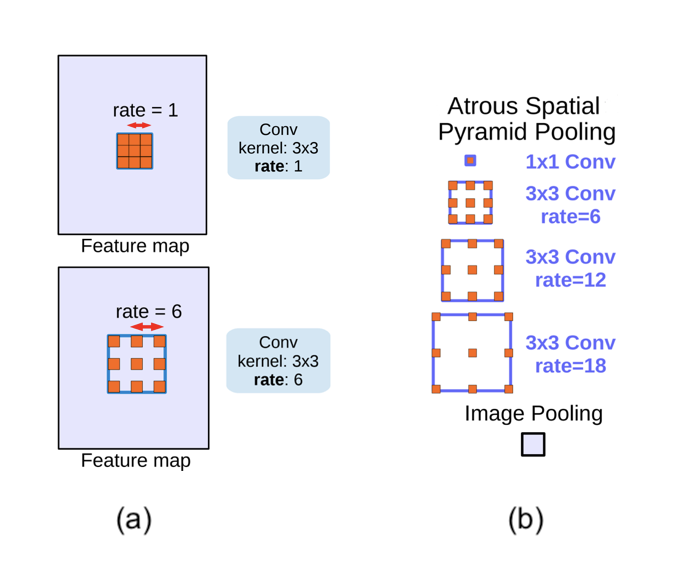
\includegraphics[width=0.5\textwidth]{figures/conv_aspp.png} %choose your uploaded image from folder "Images"
  \caption{(a) Atrous convolution, (b) ASPP augmented with Image Pooling (or Image-level features) ~\cite{chen2017rethinking}} %figure caption
  \label{fig:aconv} %labelling for internal reference
\end{wrapfigure}
One of the latest models in this family, DeepLabv3~\cite{chen2017rethinking}, applies several parallel atrous convolutions with different atrous rates
(Atrous Spatial Pyramid Pooling, or ASPP, Figure~\ref*{fig:aconv} b) to effectively capture multi-scale information. 
Image-level features, or image pooling, are also applied to incorporate global context information. Those are calculated by applying global average pooling on the last feature map of the backbone.
After applying all the operations in parallel, the results of each operation along the channel is concatenated and 1$\times$1 convolution is applied to get the output.
The addition of atruos convolutions allows the enlargement of the field of view without
increasing the size of the filtering kernel, therefore the computation time.
\subsubsection{DeepLabv3+}
The reproduction of shape contours during semantic image segmentation remained difficult with DeepLabv3~\cite{chen2018encoder}.
DeepLabv3 bilinearly upsamples the logits both during training and evaluation (Fig.~\ref*{fig:deeplab} a), hence
the improvements were made to employ the encoder-decoder structure (Figure~\ref*{fig:deeplab}) to avoid using a naive decoder.
\begin{figure}[h] %h=here; t=top; b=bottom of the page
  \centering
  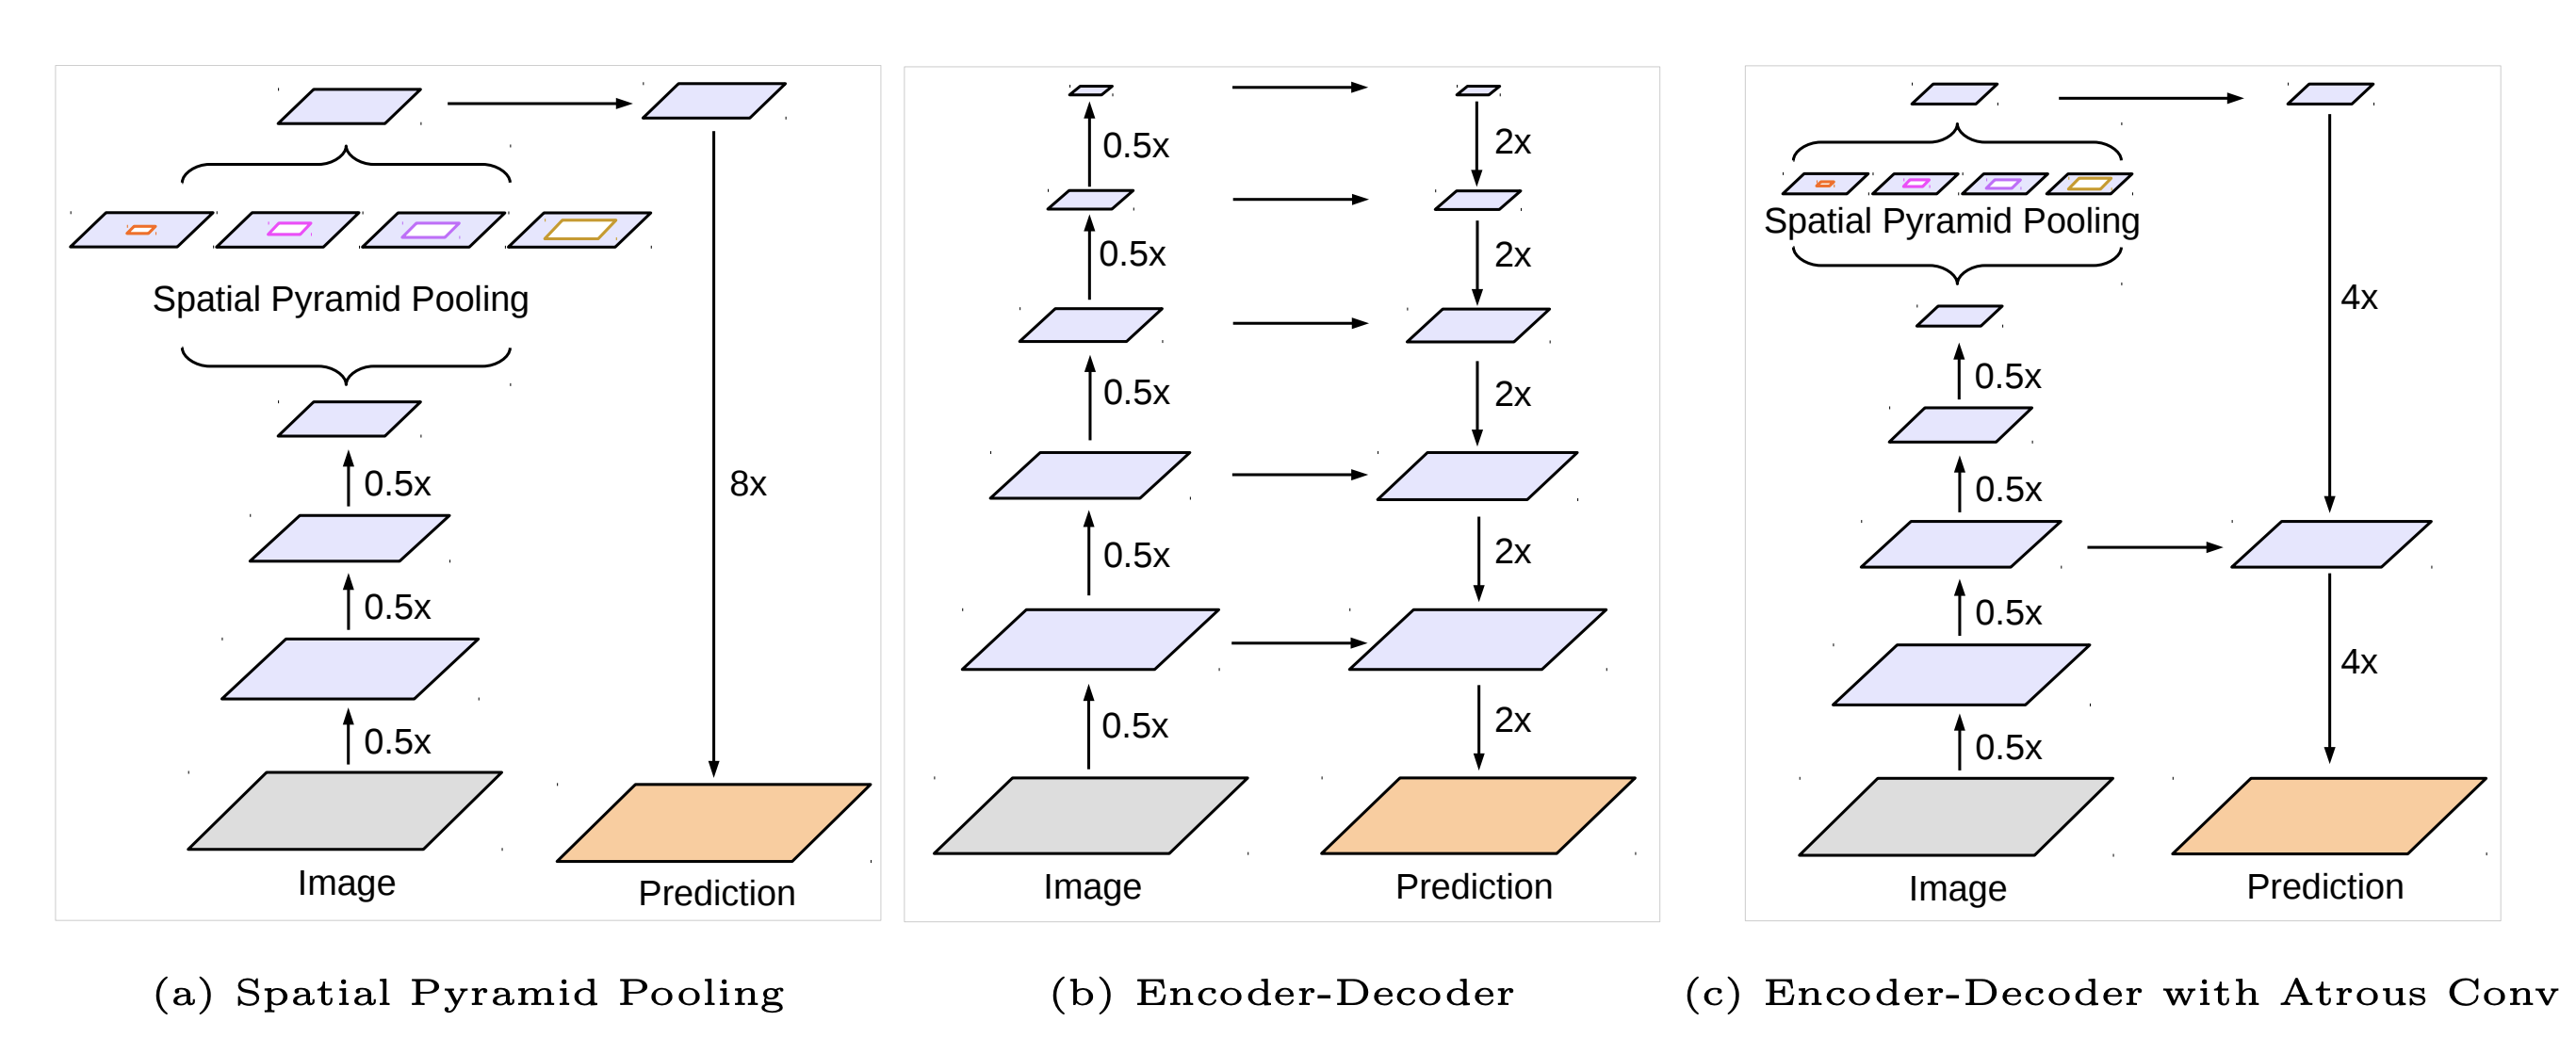
\includegraphics[width=0.9\textwidth]{figures/deeplab_encoderdecoder.png} %choose your uploaded image from folder "Images"
  \caption{The spatial pyramid pooling module of DeepLabv3 (a), the encoder-decoder structure (b) and DeepLabv3+ adaptation (c) \cite{chen2018encoder}} %figure caption
  \label{fig:deeplab} %labelling for internal reference
\end{figure} 
DeepLabv3+~\cite{chen2018encoder} adds the decoder module on top of the encoder output, as shown in Fig.~\ref*{fig:deeplabv3plus}.
In the decoder module, the 1$\times$1 convolution reduces the channels of the
low-level feature map from the encoder module which is then concatenated with the
DeepLabv3 feature map and the 3$\times$3 convolution obtains sharper segmentation results.
As a result, DeepLabv3+ holds rich semantic information from the encoder module,
while the detailed object boundaries are recovered by the decoder module and the spatial information is retrieved.
\begin{figure}[h] %h=here; t=top; b=bottom of the page
  \centering
  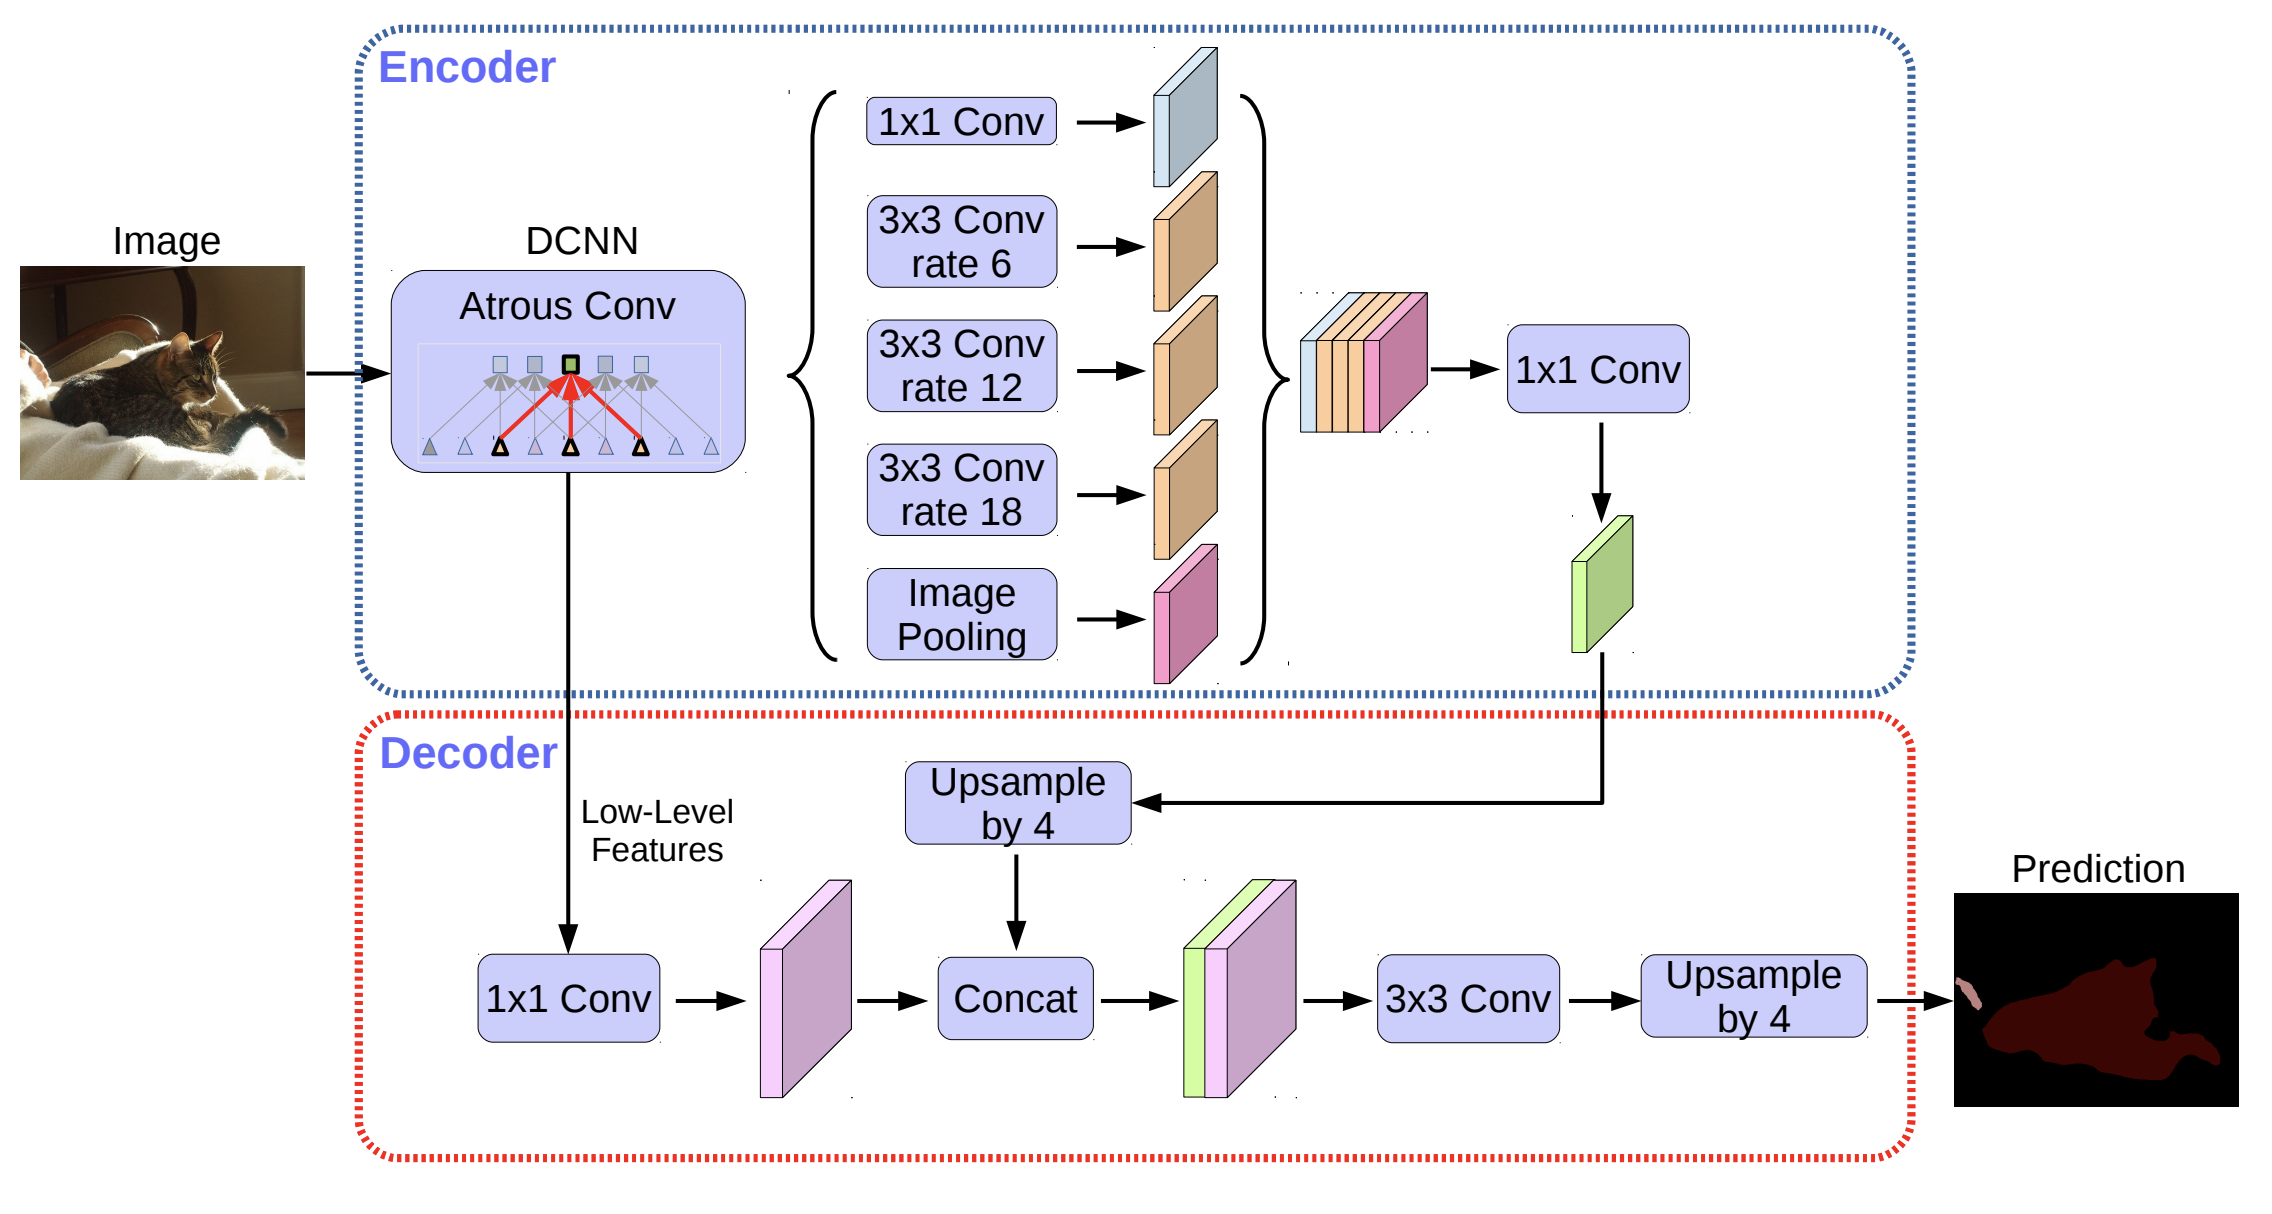
\includegraphics[width=0.9\textwidth]{figures/deeplabv3plus.png} %choose your uploaded image from folder "Images"
  \caption{DeepLabv3+ architecture. DeepLabv3 as encoder and proposed decoder structure for semantic image segmentation. \cite{chen2018encoder}} %figure caption
  \label{fig:deeplabv3plus} %labelling for internal reference
\end{figure} 

\subsection{Transformers}
\label{trans}
Transformers~\cite{vaswani2017attention} were originally designed for the neural machine translation
problem in NLP to capture long-range dependencies among words in a sentence.
Their architecture converts one sequence into another one based on encoder-decoder architecture,
but it differs from the previously existing sequence-to-sequence models because
it does not imply any Recurrent Networks. 
\begin{wrapfigure}{r}{0.45\textwidth}
  \centering
  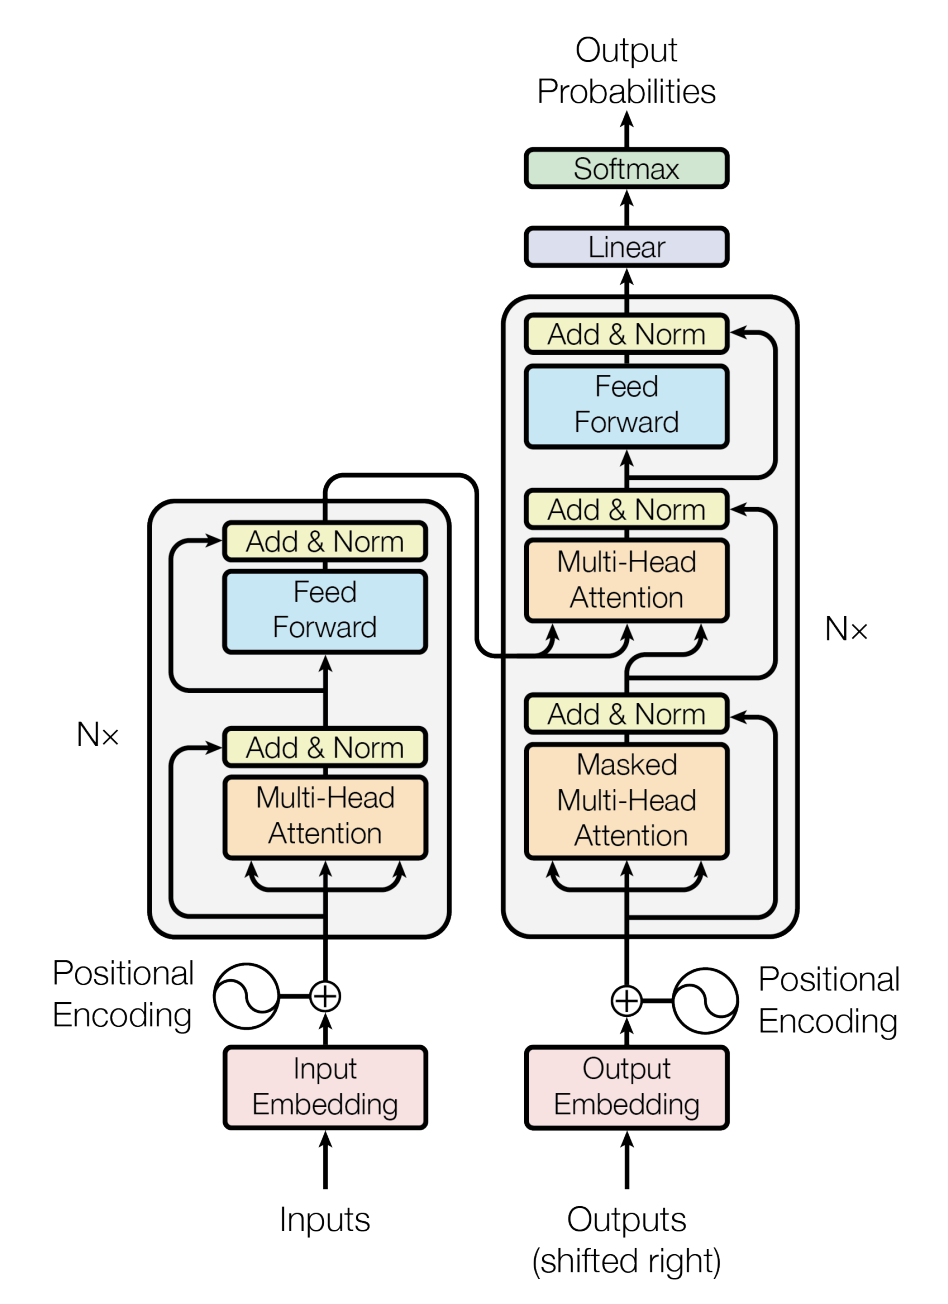
\includegraphics[width=0.4\textwidth]{figures/03_transformer_overview.png}
  \caption{Transformer model architecture. \cite{vaswani2017attention}}
  \label{fig:trans_arch}
\end{wrapfigure}
The input and output are first embedded into an $n$-dimensional space.
Since the network and the self-attention are permutation invariant,
the positional encoding is added to create a representation of the position of the word in the sentence.
The following modules consist mainly of Multi-Head Attention and Feed Forward layers. 
Encoder (Figure~\ref{fig:trans_arch}, left) and decoder (Figure~\ref{fig:trans_arch}, right)
are composed of those modules that can be stacked on top of each other $N\times$ times.

Self-attention is a sequence-to-sequence operation.
It takes a weighted average over all the input vectors using dot product.
Scaled Dot-Product Attention (Figure~\ref{fig:trans_attn}, left) can be described by the following equation:
\begin{equation} \label{eq:1}
Attention(Q,K,V) = softmax(\frac{QK^T}{\sqrt{d_k}})V
\end{equation}
where, in the context ot translation problem,
$Q$ is a matrix of vector representation of one word in the sequence,
$K$ contains vector representations of all the words in the sequence and
$V$ contains again the vector representations of all the words in the sequence.
For the multi-head attention modules in the encoder and decoder,
$V$ consists of the same word sequence as $Q$.
However, for the attention module that is taken into account,
the encoder \underline{and} the decoder sequences, $V$ and $Q$ are different.
$Q$, $K$ and $V$ matrices are used to calculate the attention scores.
These scores measure how much attention needs
to be placed on words of the input sequence with respect to a word at a certain position.
The scaling factor $\sqrt{d_k}$ is applied to avoid large values that after 
applying softmax would lead to vanishing gradients.

While Scaled Dot-Product Attention focuses on the whole sentence, 
Multi-Head Attention approaches different segments of the words.
The word vectors are divided into a fixed number (number of heads) of parts,
and then within Multi-Head Attention (Figure~\ref{fig:trans_attn}, right) 
the attention mechanism is repeated multiple times on those separate parts with linear projections of $Q$, $K$, and $V$.
Since the Feed-Forward layer is expecting just one matrix, a vector for each word,
the outputs are linearly concatenated.
This allows the system to learn from different representations of $Q$, $K$, and $V$.

\begin{figure}[h] %h=here; t=top; b=bottom of the page
    \centering
    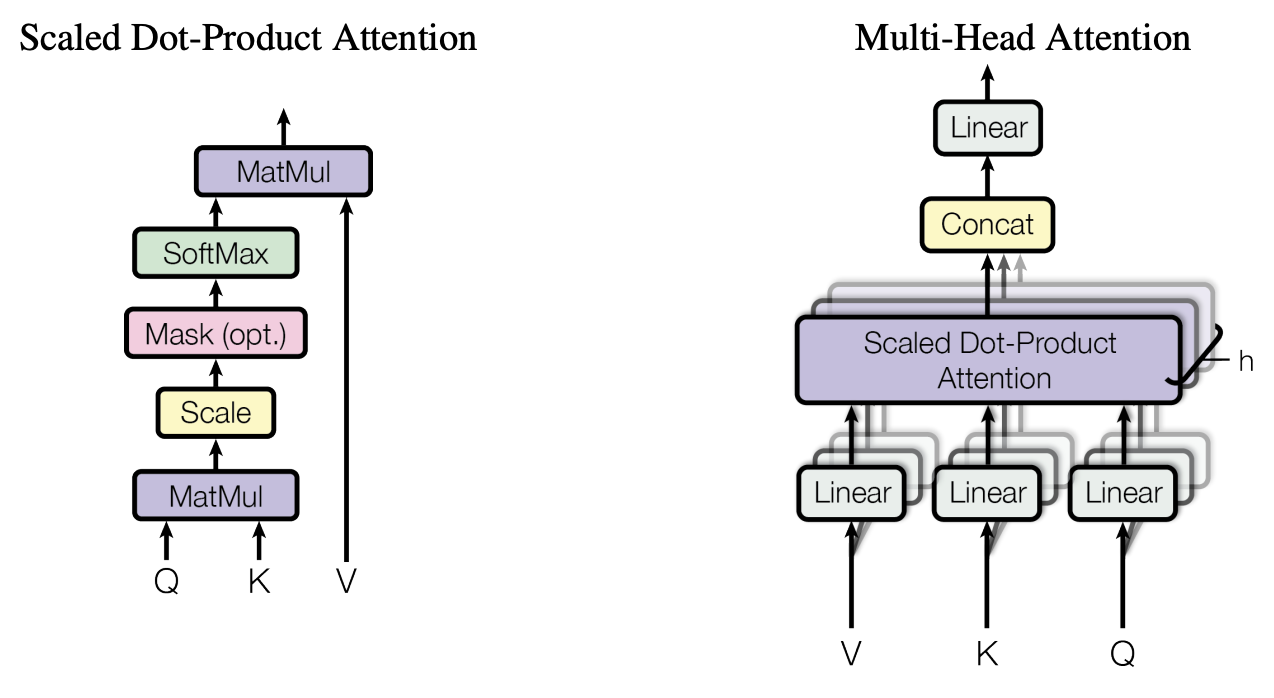
\includegraphics[width=0.7\textwidth]{figures/03_blocks_overview.png} %choose your uploaded image from folder "Images"
    \caption{Scaled Dot-Product Attention (left). Multi-Head Attention consists of several attention layers running in parallel (right). \cite{vaswani2017attention}} %figure caption
    \label{fig:trans_attn} %labelling for internal reference
\end{figure} 

To add element-wise non-linearity transformation of incoming vectors, 
the transformer includes feed-forward networks.
It processes the output from one attention layer so that it fits better for the next attention layer.
Each of the layers in the encoder and decoder contains a fully
connected feed-forward network, which is applied to each position separately and identically.
These feed-forward layers can be described as a separate, identical linear transformation of each element from the given sequence.

Naive application of transformers approach into the image domain would require evaluation of relations between each pixel and every other pixel, which is obviously not scalable. The Visual transformer (ViT) \cite{dosovitskiy2020image} is the first work to prove that a pure Transformer can achieve state-of-the-art performance in image classification. ViT converts the input image into a 1D series by cutting it into patches and feeding it to a linear layer. It yields a patch embedding. Position embeddings are added to the image patch embeddings. Adding the learnable position embeddings to each patch allows the model to learn the structure of the image. The rest of the pipeline is a standard encoder and decoder blocks of the transformer.  The decoder learns to map patch-level encodings coming from the encoder to patch-level class scores. Next, these patch-level class scores are upsampled by bilinear interpolation to pixel-level scores.

\subsubsection{SegFormer}
SegFormer~\cite{xie2021segformer} is a positional-encoding-free transformer based semantic segmentation method. As depicted in Figure \ref{fig:segformer_over}, it consists of two main modules: a hierarchical Transformer encoder to generate high-resolution coarse features and low-resolution fine features, and a lightweight All-MLP decoder to fuse these multi-level features and produce the final semantic segmentation mask. 

\begin{figure}[h] %h=here; t=top; b=bottom of the page
    \centering
    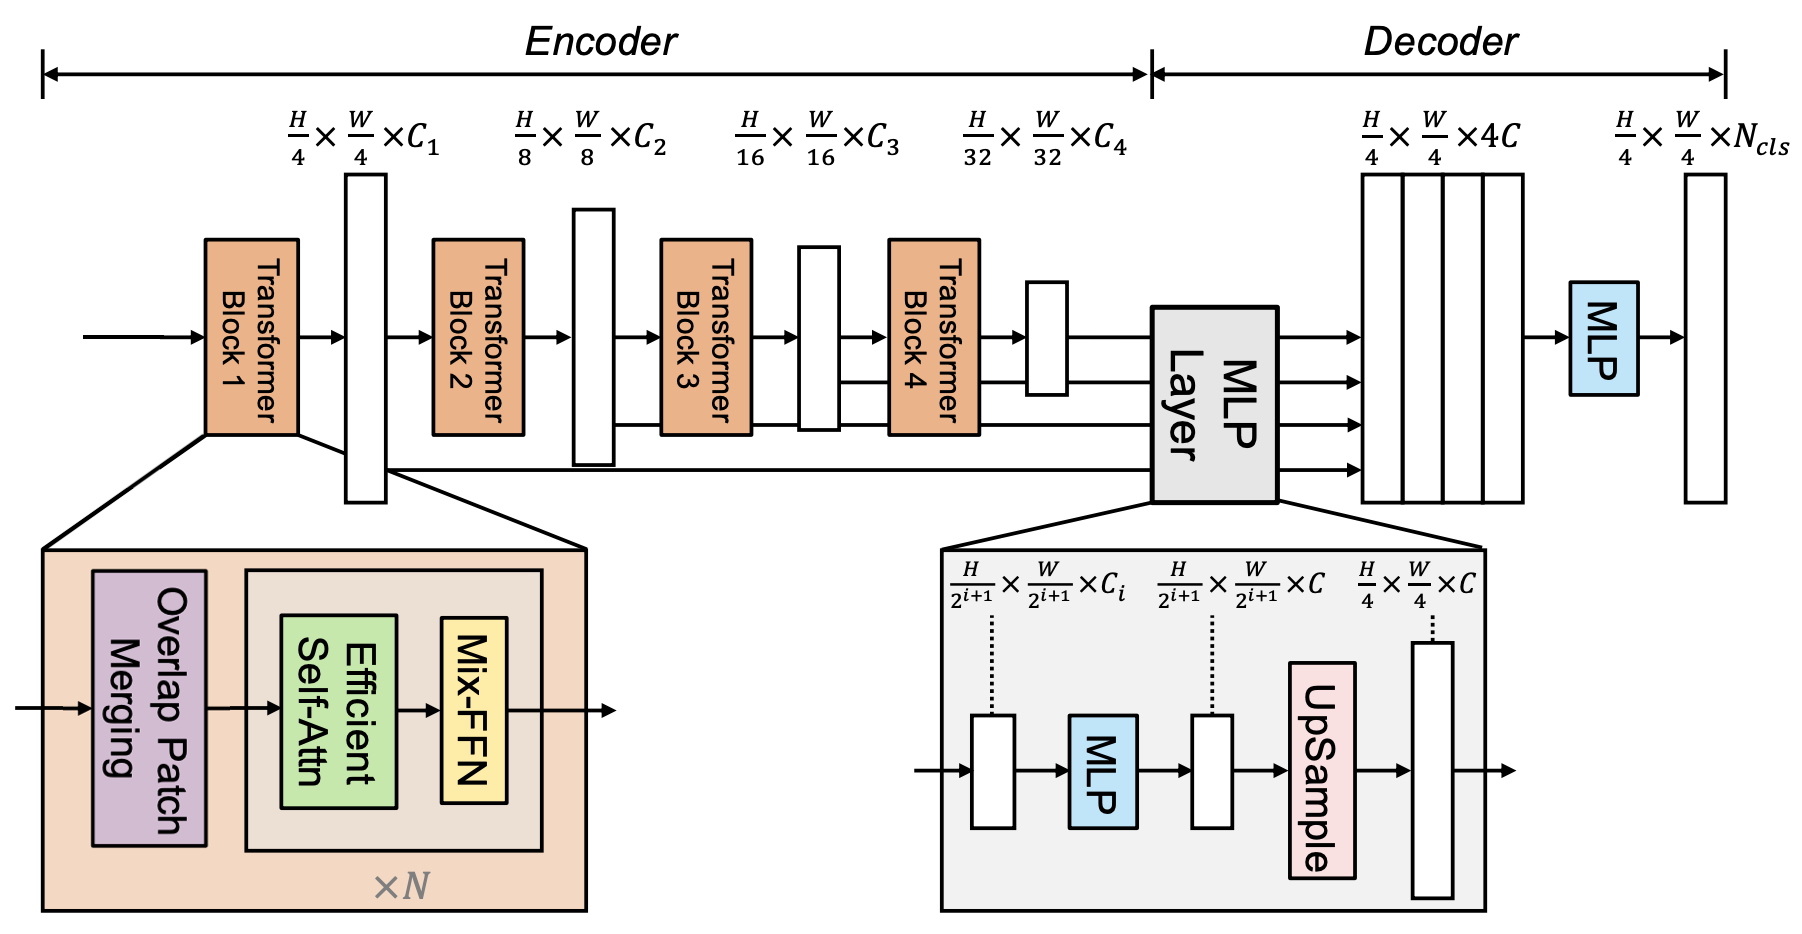
\includegraphics[height=60mm]{figures/03_segformer_overview.png} %choose your uploaded image from folder "Images"
    \caption{SegFormer consists of two main modules: A hierarchical Transformer encoder to extract coarse and fine features; and a lightweight All-MLP decoder to directly fuse these multi-level features and predict the semantic segmentation mask. “FFN” indicates feed-forward network. (modified image \cite{xie2021segformer} according to the official implementation)} %figure caption
    \label{fig:segformer_over} %labelling for internal reference
\end{figure} 

The $H\times W \times 3$ input image is forwarded to the hierarchical Transformer encoder to obtain multi-level features at $\frac{1}{4}, \frac{1}{8}, \frac{1}{16}, \frac{1}{32}$ resolution after passing through four transformer blocks.
Each transformer block consists of three modules: Overlap Patch Merging, and classical transformer building blocks: Self-Attention and Feed-forward network.

The standard transformer receives input as a 1D sequence (such as word embeddings in the previous chapter~\ref*{trans}).
To handle images, those need to be reshaped into a sequence of flattened 2D patches.
Overlapped Patch Merging produces features given an image and parameters: patch size $K$, stride between two adjacent patches $S$, and padding size $P$.
In the original paper~\cite{xie2021segformer} those are set to $K = 7$, $S = 4$ and $P = 3$.
Therefore the input is split into fixed-size patches, which then go through a linear projection.
The result is a hierarchical feature map $F_i$ with a
resolution $\frac{H}{2^{i+1}} \times \frac{W}{2^{i+1}} \times C_i$
where $i \in \{ 1,2,3,4\}$ and $C_{i+1}$ is larger than $C_i$.
By performing this with overlapped patches SegFormer aims to preserve the local continuity around those patches.

The main computation bottleneck of each transformer block in encoder is the self-attention layer. In SegFormer, before applying the self-attention according to the formula~\ref{eq:1}, the sequence $K$ is reduced by ratio $R$:
$$\hat{K} = Reshape(\frac{N}{R}, C\cdot R)(K)$$
$$K = Linear(C \cdot R, C)(\hat{K})$$
where $N = H \times W$, $Reshape(\frac{N}{R}, C \cdot R)(K)$ refers to reshaping $K$ to the the shape of $\frac{N}{R} \times (C \cdot R)$, and $Linear(C \cdot R, C)(\hat{K})$ refers to a linear layer taking a $(C \cdot R)$-dimensional tensor as input and generating a $C$-dimensional tensor as output. Therefore, the new $K$ has dimensions $\frac{N}{R} \times C$. 
In original experiments, $R$ was set to $[64, 16, 4, 1]$ from stage-1 to stage-4 and
resulted a reduction of complexity of the self-attention mechanism.

Mix-FFN (feed-forward network) can be formulated as:
$$x_{out} = MLP(GELU(Conv 3\times 3(MLP(x_{in})))) + x_{in}$$
where $x_{in}$ is the feature from the self-attention module. By using $3 \times 3$ convolution and zero padding in feed-forward network SegFormer aims to leak pixel location information since it is a positional-encoding-free method.


The multi-level features are then passed to All-MLP decoder to predict the segmentation mask at $\frac{H}{4}\times \frac{W}{4}\times N_{cls}$ resolution, where $N_{cls}$ is the number of classes.
The proposed All-MLP decoder consists of four main steps. First, multi-level features from
the encoder go through an MLP layer to unify the channel dimension (\ref{eq:2}). Then, features are up-sampled to $\frac{1}{4}$th of the original image (\ref{eq:3}). Third, a MLP layer is adopted to fuse the concatenated features (\ref{eq:4}). Finally, another MLP layer takes the fused feature to predict the segmentation mask (\ref{eq:5}).
\begin{equation} \label{eq:2}
\hat{F_i} = MLP(C_i, C)(F_i), \forall i
\end{equation}
\begin{equation} \label{eq:3}
\hat{F_i} = Upsample(\frac{H}{4}\times \frac{W}{4})(\hat{F_i}), \forall i
\end{equation}
\begin{equation} \label{eq:4}
F = MLP(4C, C)(MLP(\hat{F_i})), \forall i
\end{equation}
\begin{equation} \label{eq:5}
M = MLP(C, N_{cls})(F)
\end{equation}
where $F_i$ is the the feature and $M$ is the final mask.

\section{Survival Analysis}
The overall survival (OS) is the primary endpoint for prognostic analysis in this thesis,
hence time to death is the event of interest. 
Survival data are generally described and modelled in terms of two related probabilities, namely survival and hazard.~\cite{clark2003survival}
The survival probability $S(t)$ is the probability that an individual survives from the time origin (in our case diagnosis of breast cancer) to a specified future time $t$.
It can be denoted as: $$S(t) = Pr(T>t) = 1-F(t) = \int_t^\infty f(x) dx $$
where $T$ is a random variable that idicates the time until the event of interest (death). $F(t)$ and $f(t)$ are the cumulative distribution function
and probability density function of $T$. 
The hazard is the probability that an individual who is under observation at a time $t$ has an event at that time:
$$h(t) = lim_{\delta t \rightarrow 0}\frac{Pr(t \leq T \leq t + \delta t | T > t)}{\delta t} = \frac{f(t)}{1-F(t)}$$
In contrast to the survivor function, which focuses on not having an event, the hazard function focuses on the event occurring. 
The cumulative hazard $H(t)$, defined as the integral of the hazard,
can be calculated using the survival probability with help of the Laplace transform:
$$ H(t) = \int_0^t h(x) dx = \int_0^t \frac{f(x)}{1-F(x)} dx = - ln(1 - F(t)) = - ln(S(t)) $$
The cumulative hazard can be interpreted as the number of events that would be expected for each individual by time $t$ if the event was a repeatable process.~\cite{clark2003survival}

\subsection{Kaplan–Meier method}
The survival probability can be estimated nonparametrically from observed survival times,
both censored and uncensored, using the Kaplan–Meier method.
The probability of being alive at time $t_i$, is calculated as:
$$S(t_i) = S(t_{i-1}) (1-\frac{d_i}{n_i})$$
where $n_i$ is the number of patients alive before $t_i$ and $d_i$ is the number of events at $t_i$. $t_0=0$ and $S(0)=1$.
The estimated probability is a step function that changes value only at the time of an event.

\subsection{Cox proportional hazard models}
$H(t)$ helps to estimate $h(t)$ and assess model validity.
\chapter{Data}
To give an overview of the data used as well as extend the scheme presented in
the Introduction chapter (Figure~\ref*{fig:workflow}), refer to Figure~\ref*{fig:data_flow}.
The following sections provide more details about the data.

\begin{figure}[h]
  \centering
  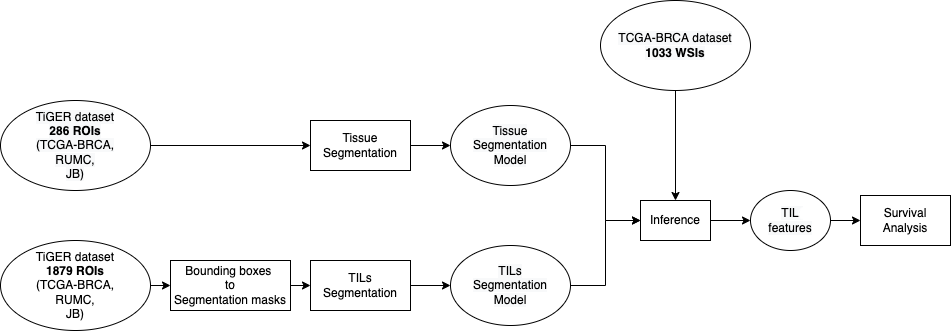
\includegraphics[width=\linewidth]{figures/data_flow.png} 
  \caption{Scheme of tasks completed in this thesis accomplimanted with the data sources and counts.} 
  \label{fig:data_flow}
\end{figure} 

\section{Segmentation}
The data for tissue and TILs segmentation originates from publicly available
Tumor InfiltratinG lymphocytes in breast cancER (TiGER) challenge dataset containing
digital pathology images of Her2 positive (Her2+) and Triple Negative (TNBC) breast
cancer whole-slide images (WSIs), regions of interest (ROIs), and manual annotations.
More specifically, the WSIROIS dataset was used for model training, validation, and
testing (see Table~\ref*{tab:segm_data}).
It includes 195 WSIs of breast cancer core-needle biopsies and surgical resections with
pre-selected ROIs and manual annotations.
TiGER data, both at WSI and ROI level, was released at a spacing (pixel size) of
approximately 0.5 \textmu m/px (at 20$\times$ magnification ), more information is available on the original
challenge website\footnote{\url{https://tiger.grand-challenge.org/Data/}}.
\begin{table}[h!]
\centering
\begin{tabular}{ l c c c c c c } 
\hline
\multirow{3}{*}{Source} &  \multicolumn{3}{c}{Tissue} & \multicolumn{3}{c}{TILs}\\ 
\cline{2-7}
 & slides & ROIs & median ROI size & slides & ROIs & median ROI size \\ 
  & & & \#pixels [k] & & & \#pixels [k] \\ 
\hline
TCGA-BRCA & 151 & 151 & 4 983 & 124 & 1744 & 20\\ 
RUMC & 26 & 81 & 1 312 & 26 & 81 & 1 312\\ 
JB & 18 & 54 & 1 465 & 18 & 54 & 1 465\\
\hline
 & 195 & 286 & & 168 & 1879 &\\
\end{tabular}
\caption{\label{tab:segm_data}TiGER data overview. Sources: Cancer Genome Atlas Breast Invasive Carcinoma (TCGA-BRCA),
Radboud University Medical Center (RUMC) and Jules Bordet Institute (JB). Tissue slides and ROIs refer to the segmentation
images and annotations whereas TILs prefix specifies the data for TILs detection provided by the challenge. }
\end{table}
The TiGER tissue annotations include eight
labels that were reduced to three (see Table~\ref*{tab:label_data}).
The training masks were generated using available XML files. In the provided mask
images, in certain cases, regions not included in ROIs and non-annotated regions in ROIs were
marked with the same label, which could not be directly used for training (see Ground truth in Figure~\ref*{fig:TCGA-GM-A2DF}).
\begin{table}[h!]
\centering
\begin{tabular}{ l c c c c } 
\hline
TiGER Tissue Label & Share & ID & new ID & new Tissue Label \\ 
\hline
Invasive tumor & 0.283 & 1 & 1 & Tumor\\ 
In-situ tumor & 0.029 & 3 & 1 & Tumor\\ 
Tumor-associated stroma & 0.286 & 2 & 2 & Stroma\\
Inflamed stroma & 0.096 & 6 & 2 & Stroma\\
Necrosis not in-situ & 0.048 & 5 & 0 & Rest\\
Healthy glands & 0.0008 & 4 & 0 & Rest\\ 
Background & 0.231 & 0 & 0 & Rest\\ 
Rest & 0.026 & 7 & 0 & Rest\\
\hline
\end{tabular}
\caption{\label{tab:label_data} Reduction of labels provided in TiGER challenge dataset. Resulting labels include three classes: Tumor (1), Stroma (2) and Rest (0) with shares of 0.312, 0.382 and 0.306. Shares were calculated by dividing
the number of pixels belonging to some label by the number of the pixel in the current image and averaged over all images. }
\end{table}

While for tissue segmentation the images and their masks could be used as directly extracted from the dataset, the data for TILs segmentation required some preprocessing. The TiGER fixed-size bounding box annotation for lymphocytes and plasma cells (see Table~\ref{tab:tils_data}) was adapted for segmentation by transforming each bounding box into an annotation of the center pixel with a dilatation of three.
\begin{table}[h!]
\centering
\begin{tabular}{ l c c c c c c } 
\hline
\multirow{2}{*}{Source} & & & & \multicolumn{3}{c}{Number of cells per ROI}\\ 
\cline{2-7}
 & \#slides & \#ROIs & \#cells & min & max & median \\ 
\hline
TCGA-BRCA & 124 & 1 744 & 19 115 & 0 (44.3\%) & 206 & 1\\ 
RUMC & 26 & 81 & 4 728 & 0 (7.4\%) & 657 & 19\\ 
JB & 18 & 54 & 5 523 & 0 (7.4\%) & 608 & 51.5\\
\hline
 & 168 & 1 879 & 29 366 & & &\\
\end{tabular}
\caption{\label{tab:tils_data} Data overview for TILs detection. Sources: Cancer Genome Atlas Breast Invasive Carcinoma (TCGA-BRCA),
Radboud University Medical Center (RUMC) and Jules Bordet Institute (JB). Number of cells here refers to the number of
bounding boxes that were assigned for lymphocytes and plasma cells, further named TILs.}
\end{table}

For the inferences the breast cancer TCGA-BRCA dataset was used, generated by
the TCGA Research Network: \hyperlink{https://www.cancer.gov/tcga}{https://www.cancer.gov/tcga}.
While there are a large number of images available in The Cancer Genome Atlas (TCGA),
only the diagnostic slide were downloaded (Formalin-Fixed Paraffin-Embedded (FFPE) slides).
FFPE slides are the gold standard in diagnostic medicine~\cite{smith_2014}.
They are prepared by fixing a specimen in formaldehyde and then placing it in a
paraffin block to section it. 
After generating a manifest file on TCGA dataset website (\cite{choosehappy_2018} for more information), which includes 1133 diagnostic slides
of BRCA breast cancer patients, the files were downloaded with the GDC Data Transfer Tool
(\verb+gdc-client+ with \verb+--manifest+ option). 


\section{Survival Analysis}
TiGER challenge aims to assess the prognostic significance of computer-generated TILs scores
for predicting survival by applying the Cox proportional hazards model. The survival analysis
is done using a large independent test dataset that includes cases from both clinical routine and from a phase 3 clinical trial, which is not directly accessible by participants. The survival analysis
within this thesis is done exclusively on publicly available TCGA-BRCA data. Where death
(\texttt{vital\_status} = 1) is considered as an event, and the time until the event or censoring is
taken either from \texttt{days\_to\_death} (number of days to death from the first diagnosis) or \texttt{days\_to\_followup}
(number of days to last follow-up from first diagnosis). 
\begin{table}[h!]
\centering
\begin{tabular}{ l c c c } 
\hline
\texttt{vital\_status} & \#cases & median age at diagnosis [years] & median time to event [months]\\ 
\hline
Dead & 146 & 62 & 37.8\\ 
Alive & 919 & 58 & 26.3\\ 
\hline
 & 1065 & 58 & 28.7\\
\end{tabular}
\caption{\label{tab:surv_data}Survival data overview.}
\end{table}
\chapter{Results \& Discussion}
\section{Tissue Segmentation}  \label{res_tissue_segm}
Three models were trained to segment the RGB input of H\&E stained image at 20$\times$ magnification
(resolution of 0.5 micron-per-pixel) into three prediction maps:
tumor, stroma, and rest (not white space, but tissue that is neither tumor nor stroma,
for details refer to Table~\ref*{tab:label_data}). The data was separated on the patient
level (or slide level, since there is one slide per patient present)
into training, validation, and test with 80\%, 10\%, and 10\% accordingly.
In order to keep the distribution of the resulting patch numbers (see Table~\ref*{tab:patch_sep})
and dataset sources fair, the patient separation in Table~\ref*{tab:patients_sep} was introduced.

\begin{table}[h!]
    \centering
    \begin{tabular}{ l c c c }
        \hline
        & Train & Validation & Test \\
        \hline
        TCGA-BRCA & 120 & 16 & 15 \\
        RUMC & 20 & 3 & 3 \\
        JB & 16 & 1 & 1 \\
        \hline
        & 156 & 20 & 19 \\
    \end{tabular}
\caption{\label{tab:patients_sep} Split of patients across different medical sources
into train, validation, and test sets for segmentation tasks.}
\end{table}

The patches were created using a sliding window approach with 256$\times$256 sized patches
and stride equals 128. The additional rotation augmentation was applied, by rotating each patch
5 times at 9 degrees each.

\begin{table}[h!]
    \centering
    \begin{tabular}{ l c c c c c c c c c}
        \hline
        & \multirow{2}{*}{slides} & \multirow{2}{*}{ROIs}& \multirow{2}{*}{patches}& \multicolumn{6}{c}{Number of patches that include}\\ 
        \cline{5-10}
        & & & & Tumor & Stroma & Rest & 1 class & 2 classes & 3 classes\\
        \hline
        Train & 156 & 228 & 220\,567 & 154\,734 & 172\,046 & 107\,506 & 63\,919 & 99\,577 & 57\,071 \\
         &  &  &  & (70\%) & (78\%) & (49\%) & (29\%) & (45\%) & (26\%) \\
        Valida- & 20 & 25 & 29\,465 & 16\,884 & 22\,187 & 13\,954 & 11\,171 & 13\,028 & 5\,266 \\
        tion &  &  &  & (57\%) & (75\%) & (47\%) & (38\%) & (44\%) & (18\%)\\
        Test & 19 & 33 & 30\,248 & 18\,194 & 25\,630 & 14\,787 & 8\,548 & 15\,037 & 6\,663\\
         &  &  &  & (60\%) & (85\%) & (49\%) & (28\%) & (50\%) & (22\%)\\
        \hline
        & 195 & 286 & 280\,280 &  &  &  & & & \\
    \end{tabular}
    \caption{\label{tab:patch_sep} Overview of patches that were split into train, validation,
    and test sets for tissue segmentation. The percentages indicate the fraction of a specific conditioned group of patches to the number of all patches in the "patches" column.}
\end{table}

The models were trained with the mmsegmentation toolbox~\cite{mmseg2020}. 
All models were trained for 160K iterations with Cross Entropy Loss and
standard data augmentation techniques including resizing at a random sample scale in the range
of (0.5, 2.0), cropping with the maximum 0.75 of a single category present, flipping with 0.5 probability,
and application of photometric distortion which includes 0.5 probability for each of the following transformations: random brightness, contrast, saturation, hue and color adjustments. 
The DeepLabv3+ model was taken as a baseline and trained with ResNet50 backbone,
Adam optimizer, learning rate equals 0.0001 and batch size of 64. Whereas the
transformer-based SegFormer-B5 (further referred to as SegFormer) architecture was trained once with the same setup of
Adam optimizer, 0.0001 learning rate and batch size of 64, and additionally, as 
in original paper~\cite*{xie2021segformer}, using AdamW optimizer, the learning rate
set to an initial value of 0.00006 and then used a poly learning rate schedule with
factor 1.0 by default.

\begin{table}[h!]
    \centering
    \begin{tabular}{ l c c c c c c c c}
        \hline
        \multirow{2}{*}{Model} & \multirow{2}{*}{FLOPs} & \multirow{2}{*}{Params} & \multirow{2}{*}{Iterations} & \multirow{2}{*}{Runtime} & \multicolumn{4}{c}{mDice}\\
        & & & & & Overall & Tumor & Stroma & Rest \\
        \hline
        DeepLabv3+ & 44.16 & 43.58 M & 160 K & 1d 12h 2m & \textbf{85.25} & 85.13 & 88.07 & 83.66\\
        SegFormer & 12.96 & 81.97 M & 160 K  & 3d 4h 30m & 83.44 & 83.83 & 86.32 & 80.16\\
        SegFormer, & \multirow{2}{*}{12.96} & \multirow{2}{*}{81.97 M} & \multirow{2}{*}{160 K} & \multirow{2}{*}{3d 4h 25m} & \multirow{2}{*}{84.93} & \multirow{2}{*}{85.40} & \multirow{2}{*}{87.40} & \multirow{2}{*}{82.00}\\
        AdamW & & & & & & & & \\
        \hline
    \end{tabular}
\caption{\label{tab:tissue_perform} Overview of the trained tissue segmentation models. The runtime is given for a training on one GPU NVIDIA A100 SXM4.}
\end{table}

\begin{figure}[H]
    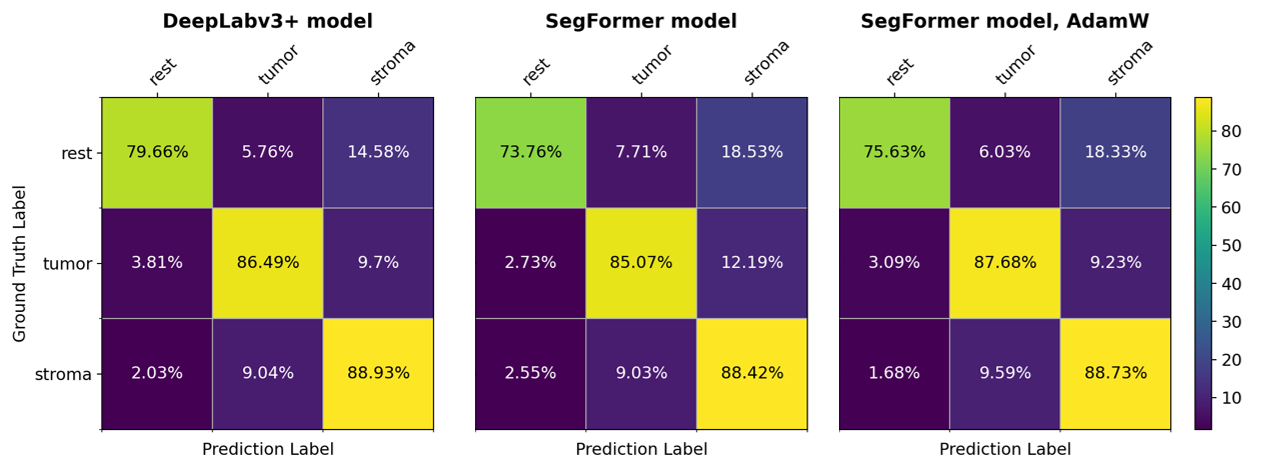
\includegraphics[width=\linewidth]{figures/tissue/conf_matrices.png}
    \caption{Confusion matrices on pixel level for DeepLabv3+, SegFormer and SegFormer with AdamW optimizer
    based on test set of 32 ROIs.}
    \label{fig:tissue_confusion}
\end{figure}

During a close investigation of test data, one slide (with the prefix TCGA-OL-A5RW-01Z-00-DX1)
was excluded from the test set due to an obvious image-mask mismatch. The overall
performance of the models, the number of parameters, and the resulting dice score after testing on 
32 test images can be found in Table~\ref*{tab:tissue_perform}. The first thing that catches the eye is the severe runtime difference of
SegFormer-based methods compared to the DeepLabv3+ accompanied by doubled number of parameters.
None of the SegFormer approaches outperform the DeepLabv3+, but the performance
is comparable, which can be also observed in the confusion matrices in Figure~\ref*{fig:tissue_confusion}.
Both SegFormer-based methods show difficulty correctly segmenting rest regions, whereas
SegFormer AdamW slightly outperforms DeepLabv3+ in the number of true positive detected tumor pixels.

As previously mentioned, the dataset originates from three medical
institutions which make it reasonable to characterize the performance separately.
The boxplots in Figure~\ref*{fig:tissue_dice_boxplots} indicate that the performance of
the DeepLabv3+ and SegFormer AdamW models in TCGA-BRCA and JB groups are fairly invariant.
Whereas the RUMC group accounts not only for the lower performance of SegFormer-based methods
in segmenting rest regions but also for an improvement of tumor region segmentation by SegFormer AdamW
model both observed in Figure~\ref*{fig:tissue_confusion}.

\begin{figure}[H]
    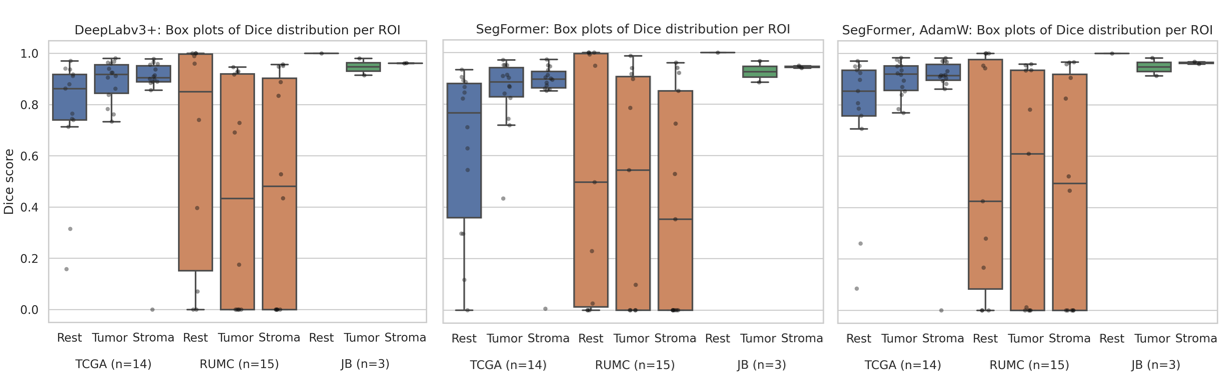
\includegraphics[width=\linewidth]{figures/tissue/dices.png}
    \caption{Boxplots of pixel wise calculated dice score across three datastes (TCGA-BRCA, RUMC, JB) and three segmentation labels.}
    \label{fig:tissue_dice_boxplots}
\end{figure} 

The additional specialty that Figure~\ref*{fig:tissue_dice_boxplots} brings to light is
the considerable number of RUMC ROIs that have been evaluated with dice scores close to
zero across all models. Due to the nature of the Dice score, those can be originated from
significant numbers of either false positives, false negatives, or both.
According to the boxplots of precision and recall in Figure~\ref*{fig:tissue_pr_r_boxplots}
the precision across all models has more close zero values that indicate more frequent
false positives. 
There are clear examples, such as Figure~\ref*{fig:TC_S01_P000159},
where the ground truth includes exclusively rest but all trained models provide multiple class predicitons.
Even though there are also opposite examples of regions that were solely annotated as rest and predicted as
such (which then lead to occasional dice, precision, and recall equal to one, see Figure~\ref*{fig:tissue_dice_boxplots}
and~\ref*{fig:tissue_pr_r_boxplots}), the issue of false positives needed to be further explored.

Out of the original 81 RUMC ROIs, 14\% of ROIs carry the annotation of only class label 7 - rest.
According to the organizers, that class contains regions of several tissue compartments that are not
specifically annotated in the other categories, such as healthy stroma, erythrocytes, adipose tissue,
skin, nipple, etc. There are none of such annotations in TCGA-BRCA or JB datasets.
After forming new masks with only three classes, the number of RUMC ROIs annotated completely as rest grew
to 17\% due to an additional ROI that represented only necrosis not in-situ.
Even though the number of all-rest-ROIs in the new TCGA-BRCA is 0.2\% and even 22\% in JB, RUMC ROIs
originally annotated as rest (label 7) need to be minded.
Those ROIs may not be the consequence of a bad annotation, but in future experiments,
it should be addressed by assigning them a reduced sampling rate, lower weights or excluding those completely. 

The patch size and the sampling stride define the overlap between consecutively extracted
patches from the WSI or ROI image. The stitching of the segmented patches introduced tiling artifacts
visible in Figure~\ref*{fig:TC_S01_P000159} and~\ref*{fig:TCGA-GM-A2DF}.
The reason might be an overfitting problem due to small patches of 256$\times$256 and
50\% overlap used for training and validation. Hence the problem can be tackled by
applying less spacing during patch formation and additional augmentations.
During inference, Khened, M et al.~\cite*{khened2021generalized} addressed a similar
problem by increasing patch size by a factor of 4 (from 256$\times$256 to 1024$\times$1024)
and keeping 50\% overlap. Due to time constraints and difficulties in migrating transformer based
models to accept generalized input, this experiment was not further pursued.

A close look at the prediction also revealed that at some cases dice scores might suffer due to some inaccuracies
in the annotations. Figure~\ref*{fig:TCGA-GM-A2DF} showcases that all models were
penalized for detecting a rest region inside of the tumor, which was probably learned
with some dependency to the presence of white space, which also present in the same slide
(the bubles in the lower part of the image) and was annotated as rest.

Nonetheless, there are positive segmentation results present, such as JB ROIs depicted in
Figure~\ref*{fig:s_250B_1} and~\ref*{fig:s_250B_2} where the performance of SegFormer AdamW
is either very close or slightly better then DeepLabv3+. 
Curiously, in Figure~\ref*{fig:s_250B_2} the SegFromer AdamW performs slightly better partly
because this model, in contrast to the rest, did not attempt to annotate the small possibly
tumorous region in the upper left corner (around (250, 200), which is not annotated in ground
truth but visually highly similar to the tumor regions in this example). To decide whether
this is an encouraging behavior the pathologist must be consulted, but in some cases,
SegFromer AdamW manages to considerably outperform DeepLabv3+, as visualized in
Figure~\ref*{fig:TCGA-EW-A1P4}. Yet while the SegFormer AdamW model remains promising, due to overall better performance and
runtime, this thesis will use the DeepLabv3+ model for further inferences and analysis.

For model inference, the model with the best pixel-wise Dice score on the validation set was used.
Patches of size 256$×\times$256 were extracted from the tissue region at 20$\times$ magnification
with a stride of 184 (for faster runtime). The whitespace was extracted by using thresholding and
inference of non-background pixels was then performed.

\begin{figure}[H]
    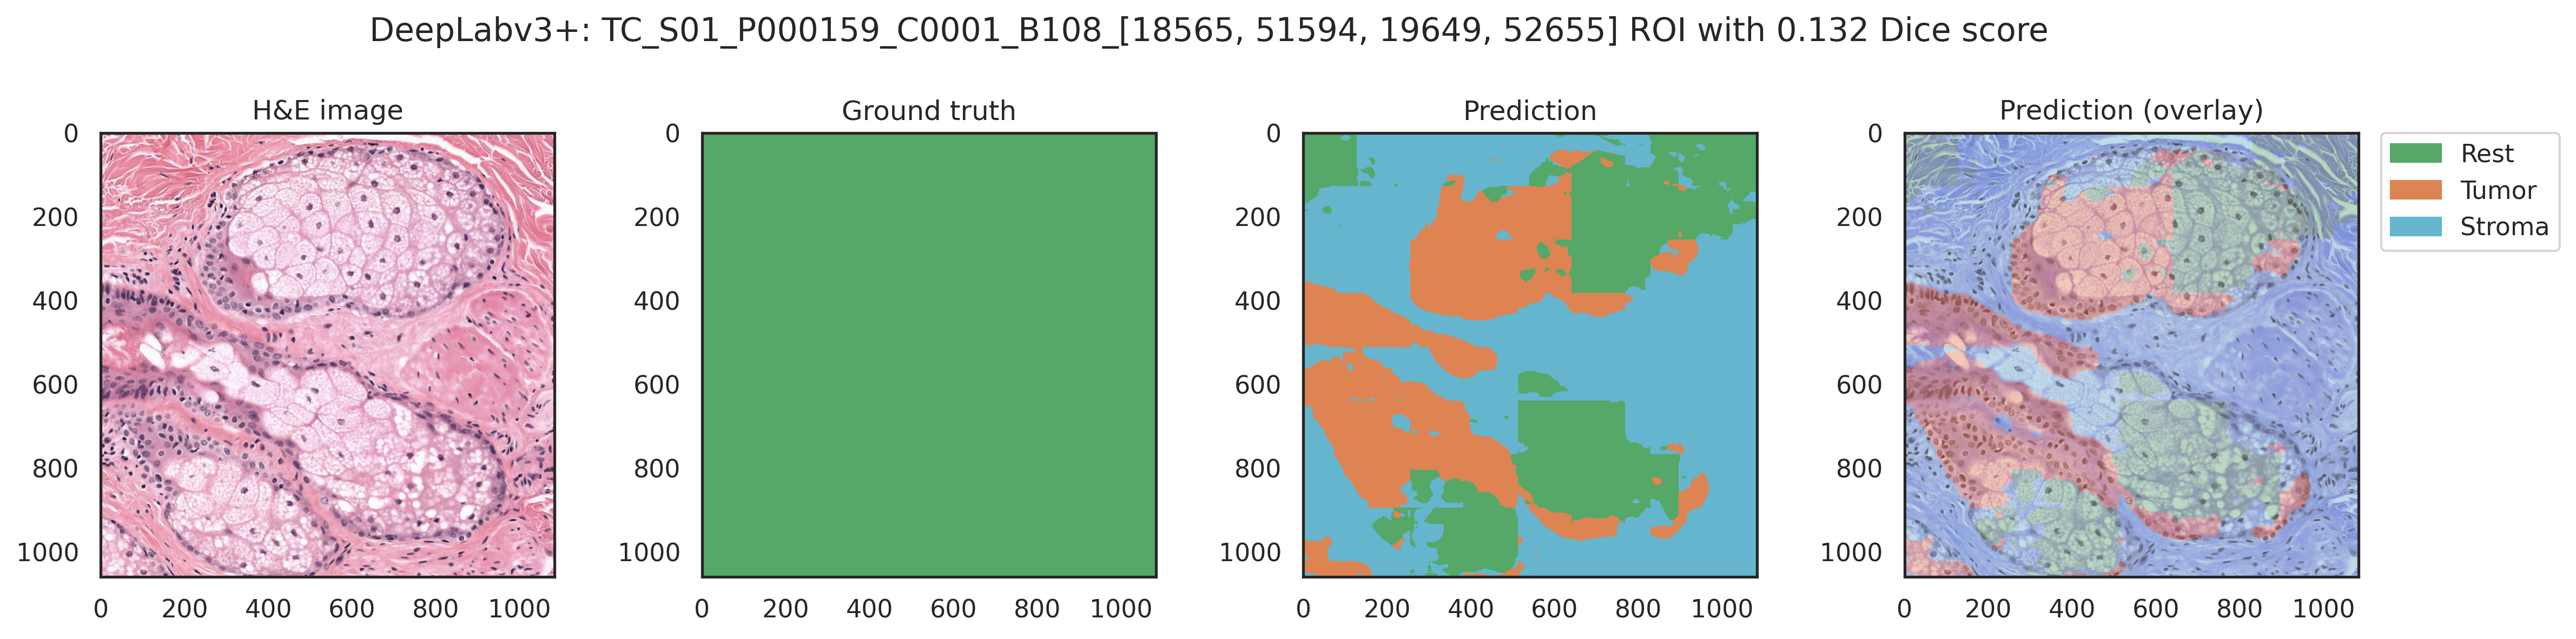
\includegraphics[width=\linewidth]{figures/tissue/deeplabv3+_dice_tc_TC_S01_P000159_C0001_B108_[18565,_51594,_19649,_52655]_check.png}
    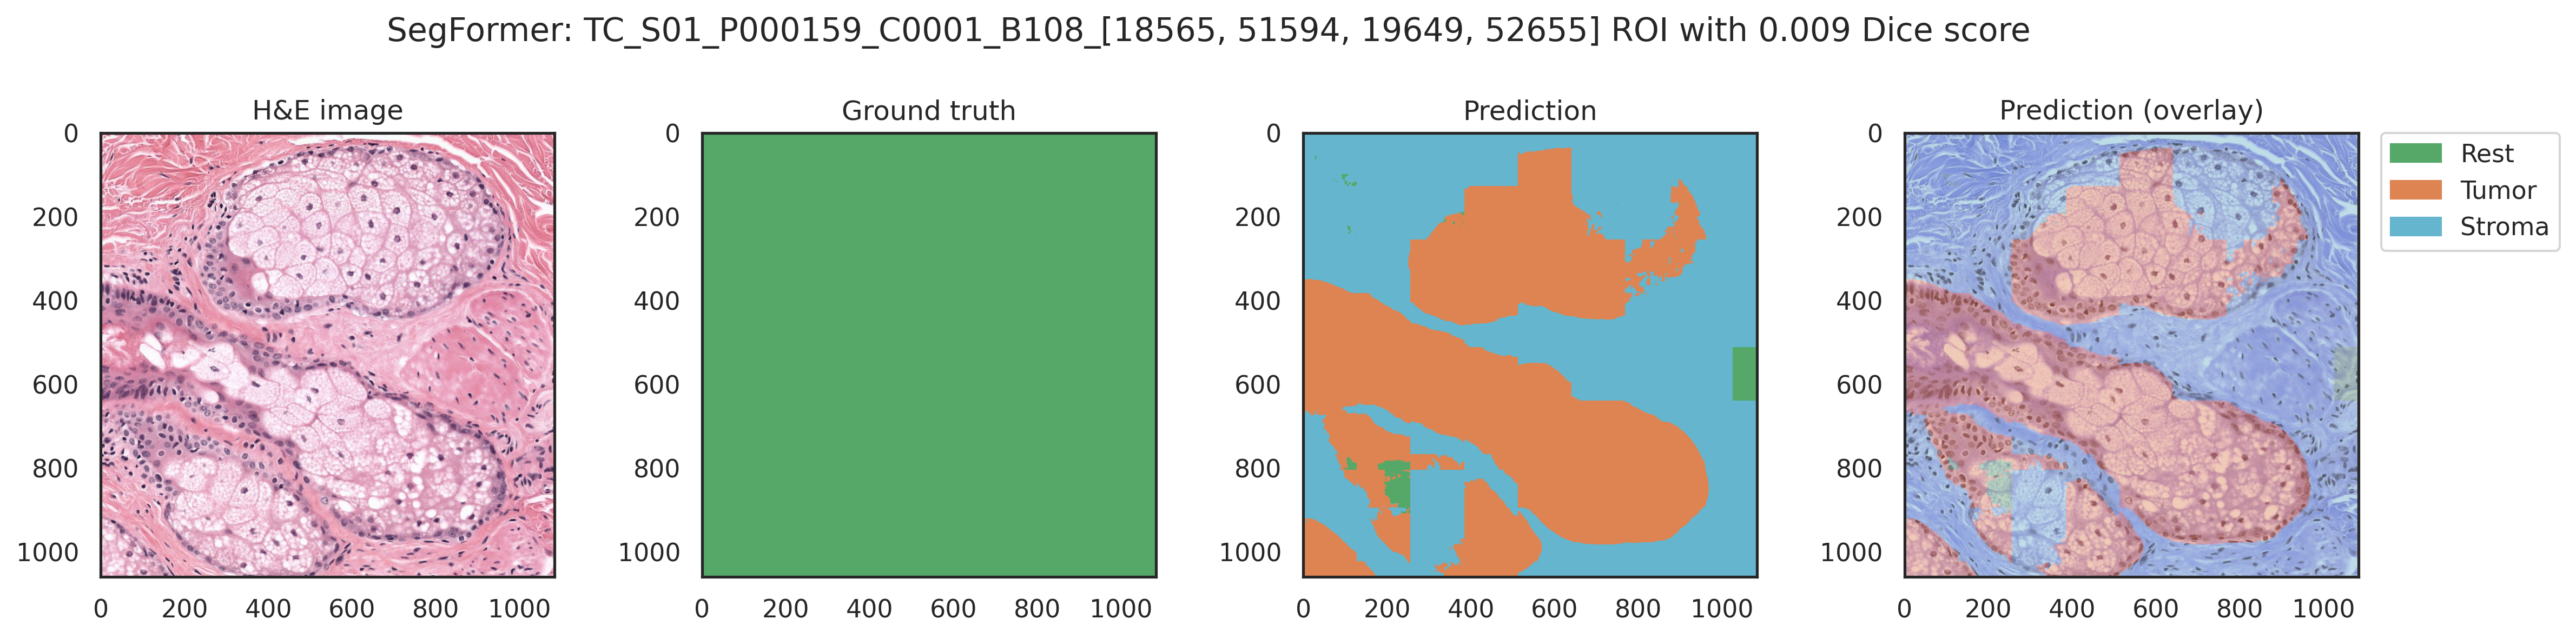
\includegraphics[width=\linewidth]{figures/tissue/segformer_dice_tc_TC_S01_P000159_C0001_B108_[18565,_51594,_19649,_52655]_check.png}
    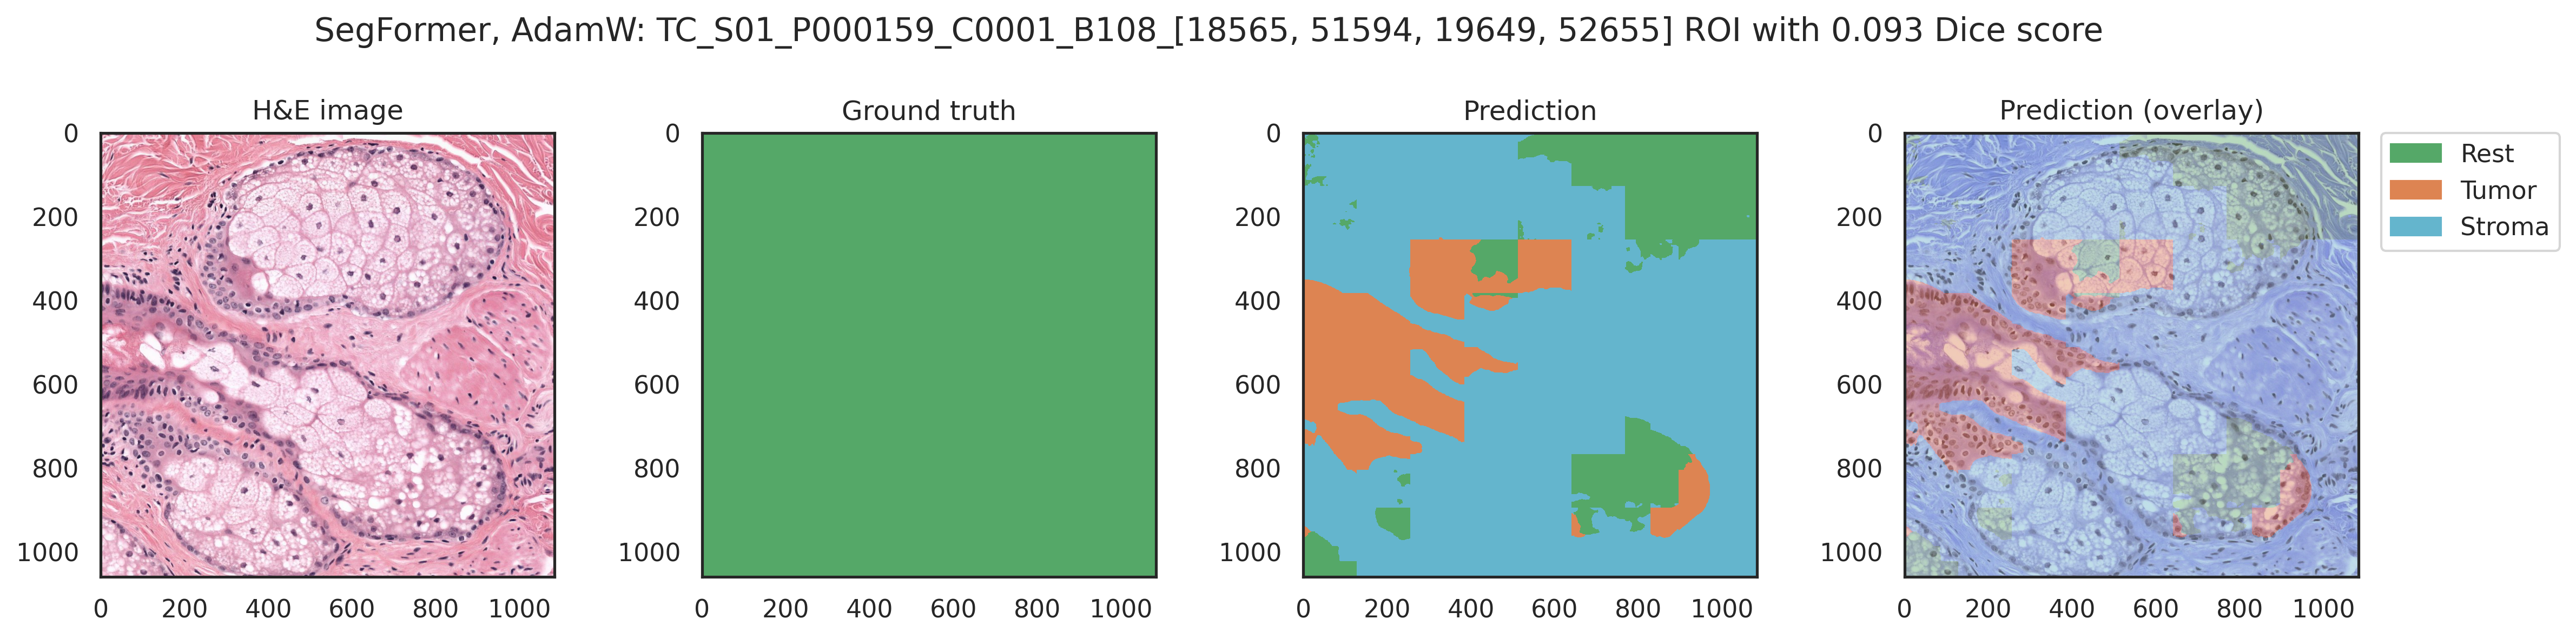
\includegraphics[width=\linewidth]{figures/tissue/segformer,_adamw_dice_tc_TC_S01_P000159_C0001_B108_[18565,_51594,_19649,_52655]_check.png}
    \caption{Example of rich false positive segmentation RUMC ROI that contributes to the cases of close zero dice scores.}
    \label{fig:TC_S01_P000159}
\end{figure}

\begin{figure}[H]
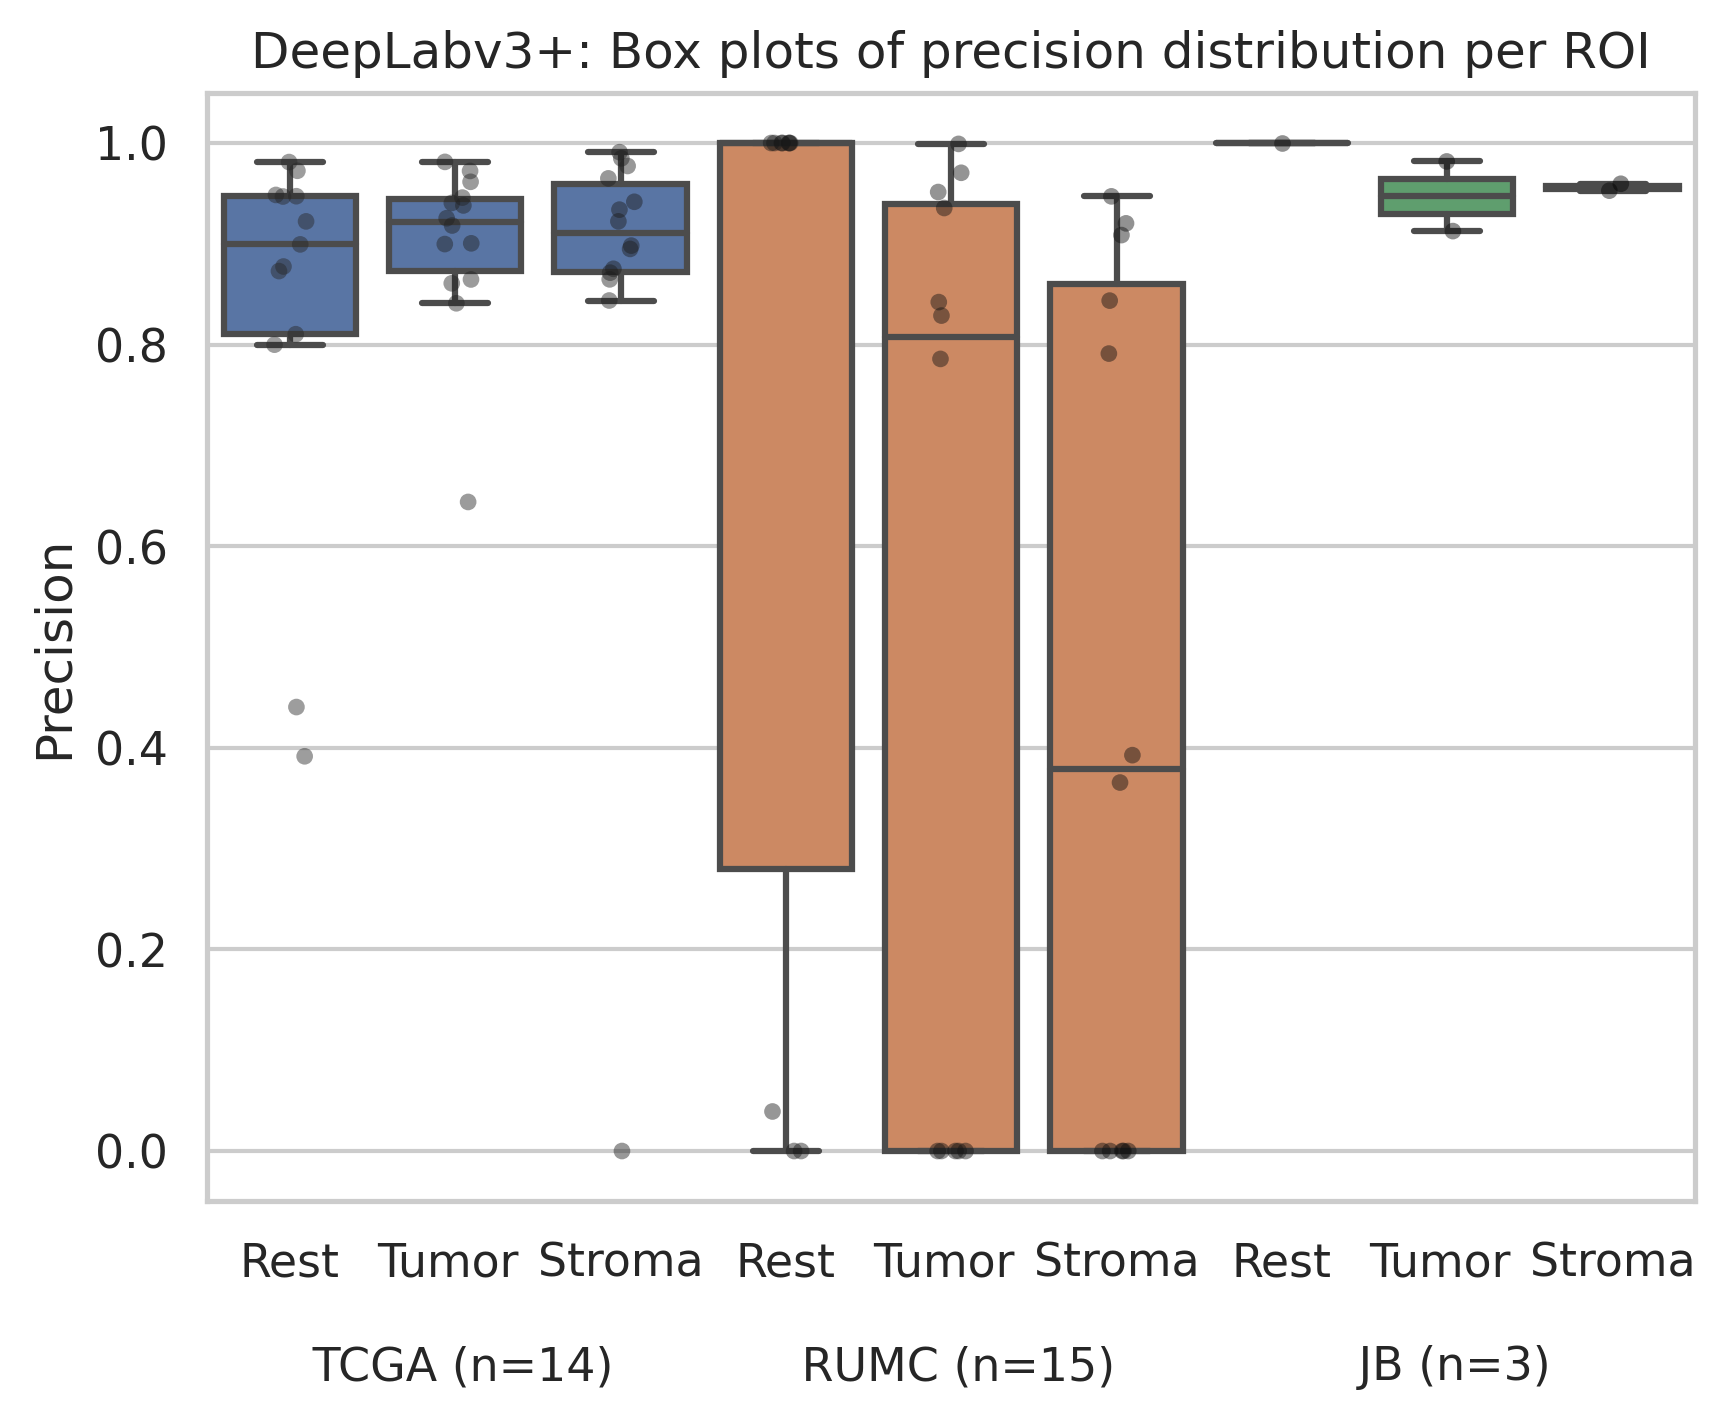
\includegraphics[width=.5\linewidth]{figures/tissue/deeplabv3+_prec_roi_wsirois.png}
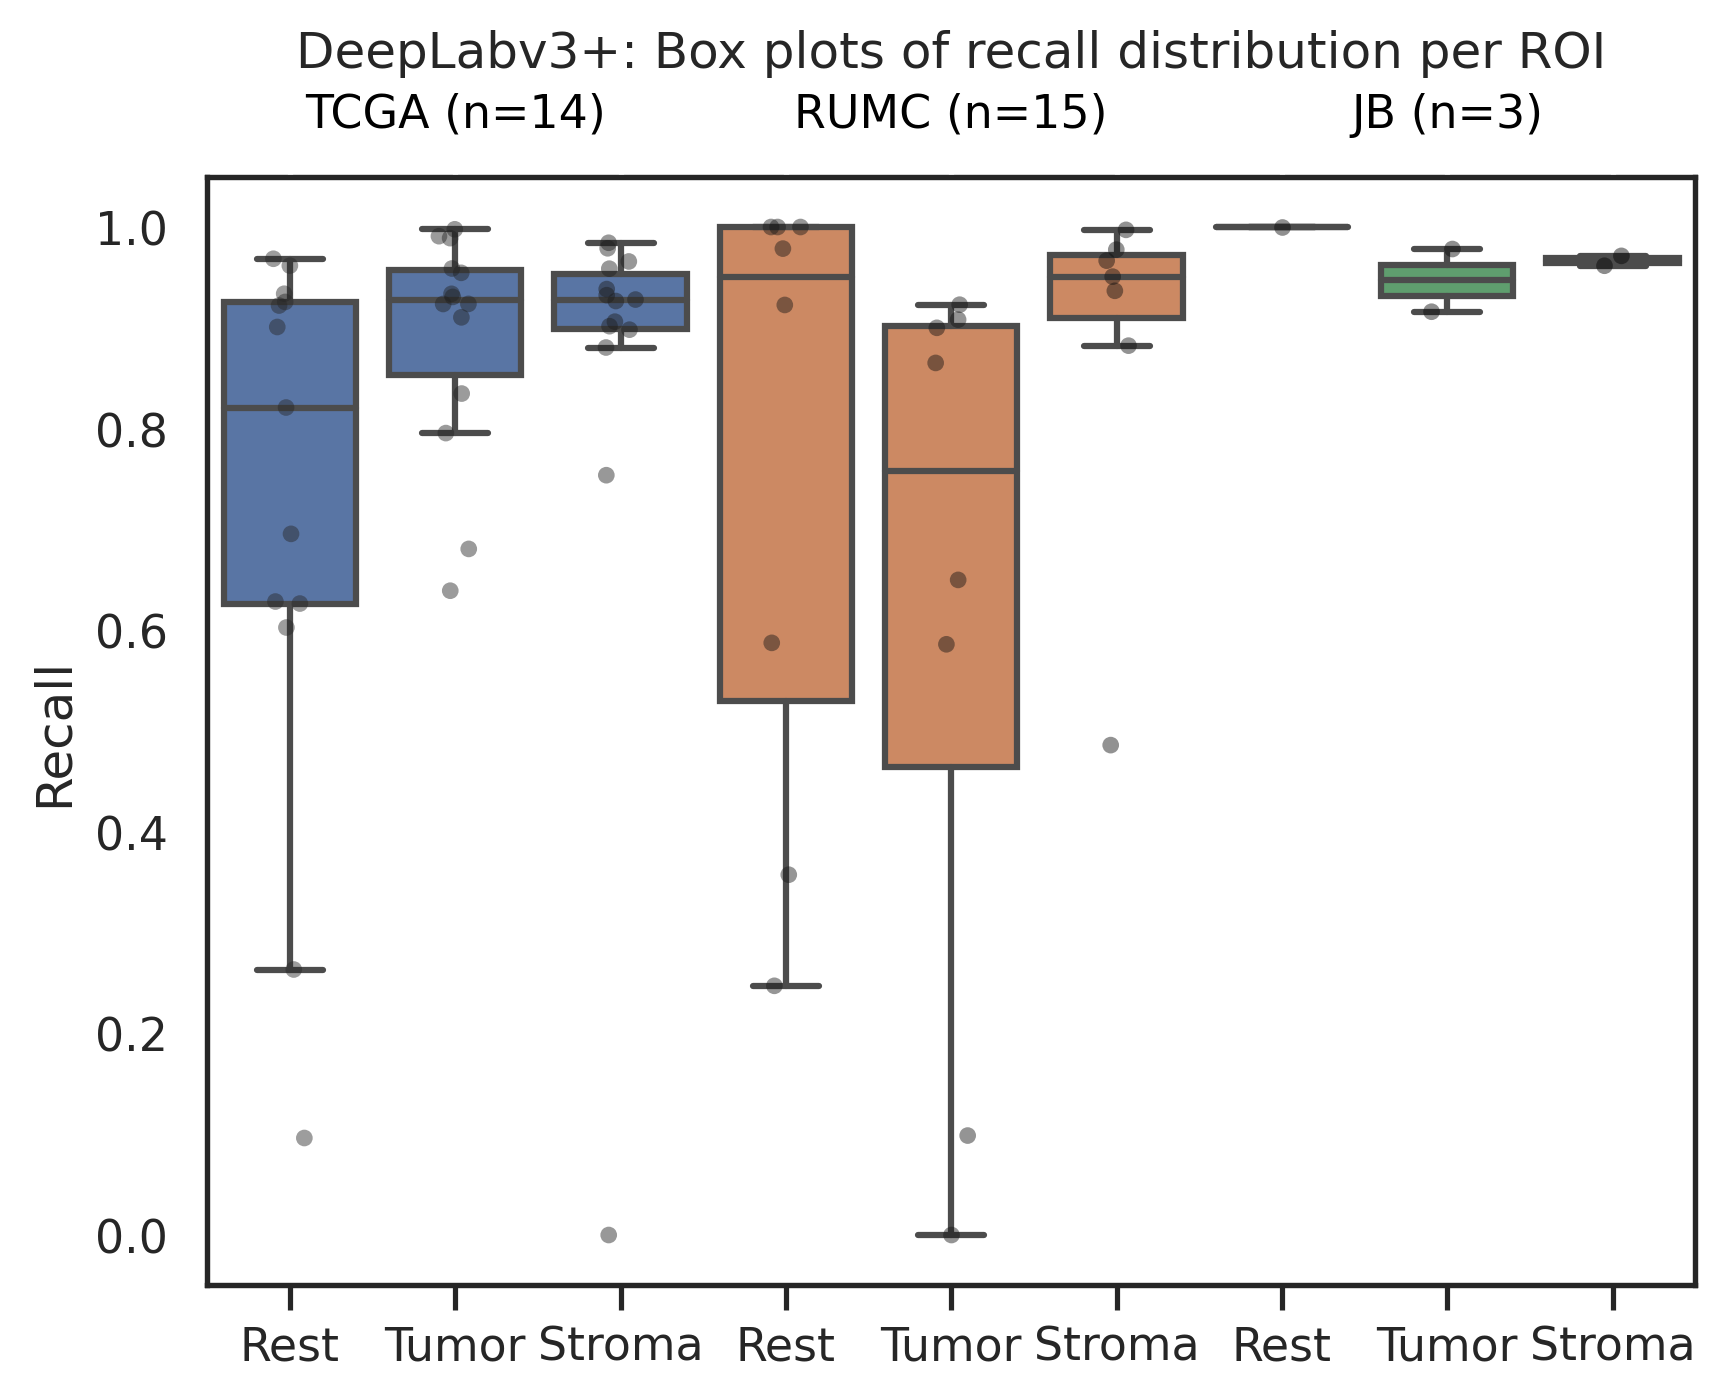
\includegraphics[width=.5\linewidth]{figures/tissue/deeplabv3+_recall_roi_wsirois.png}

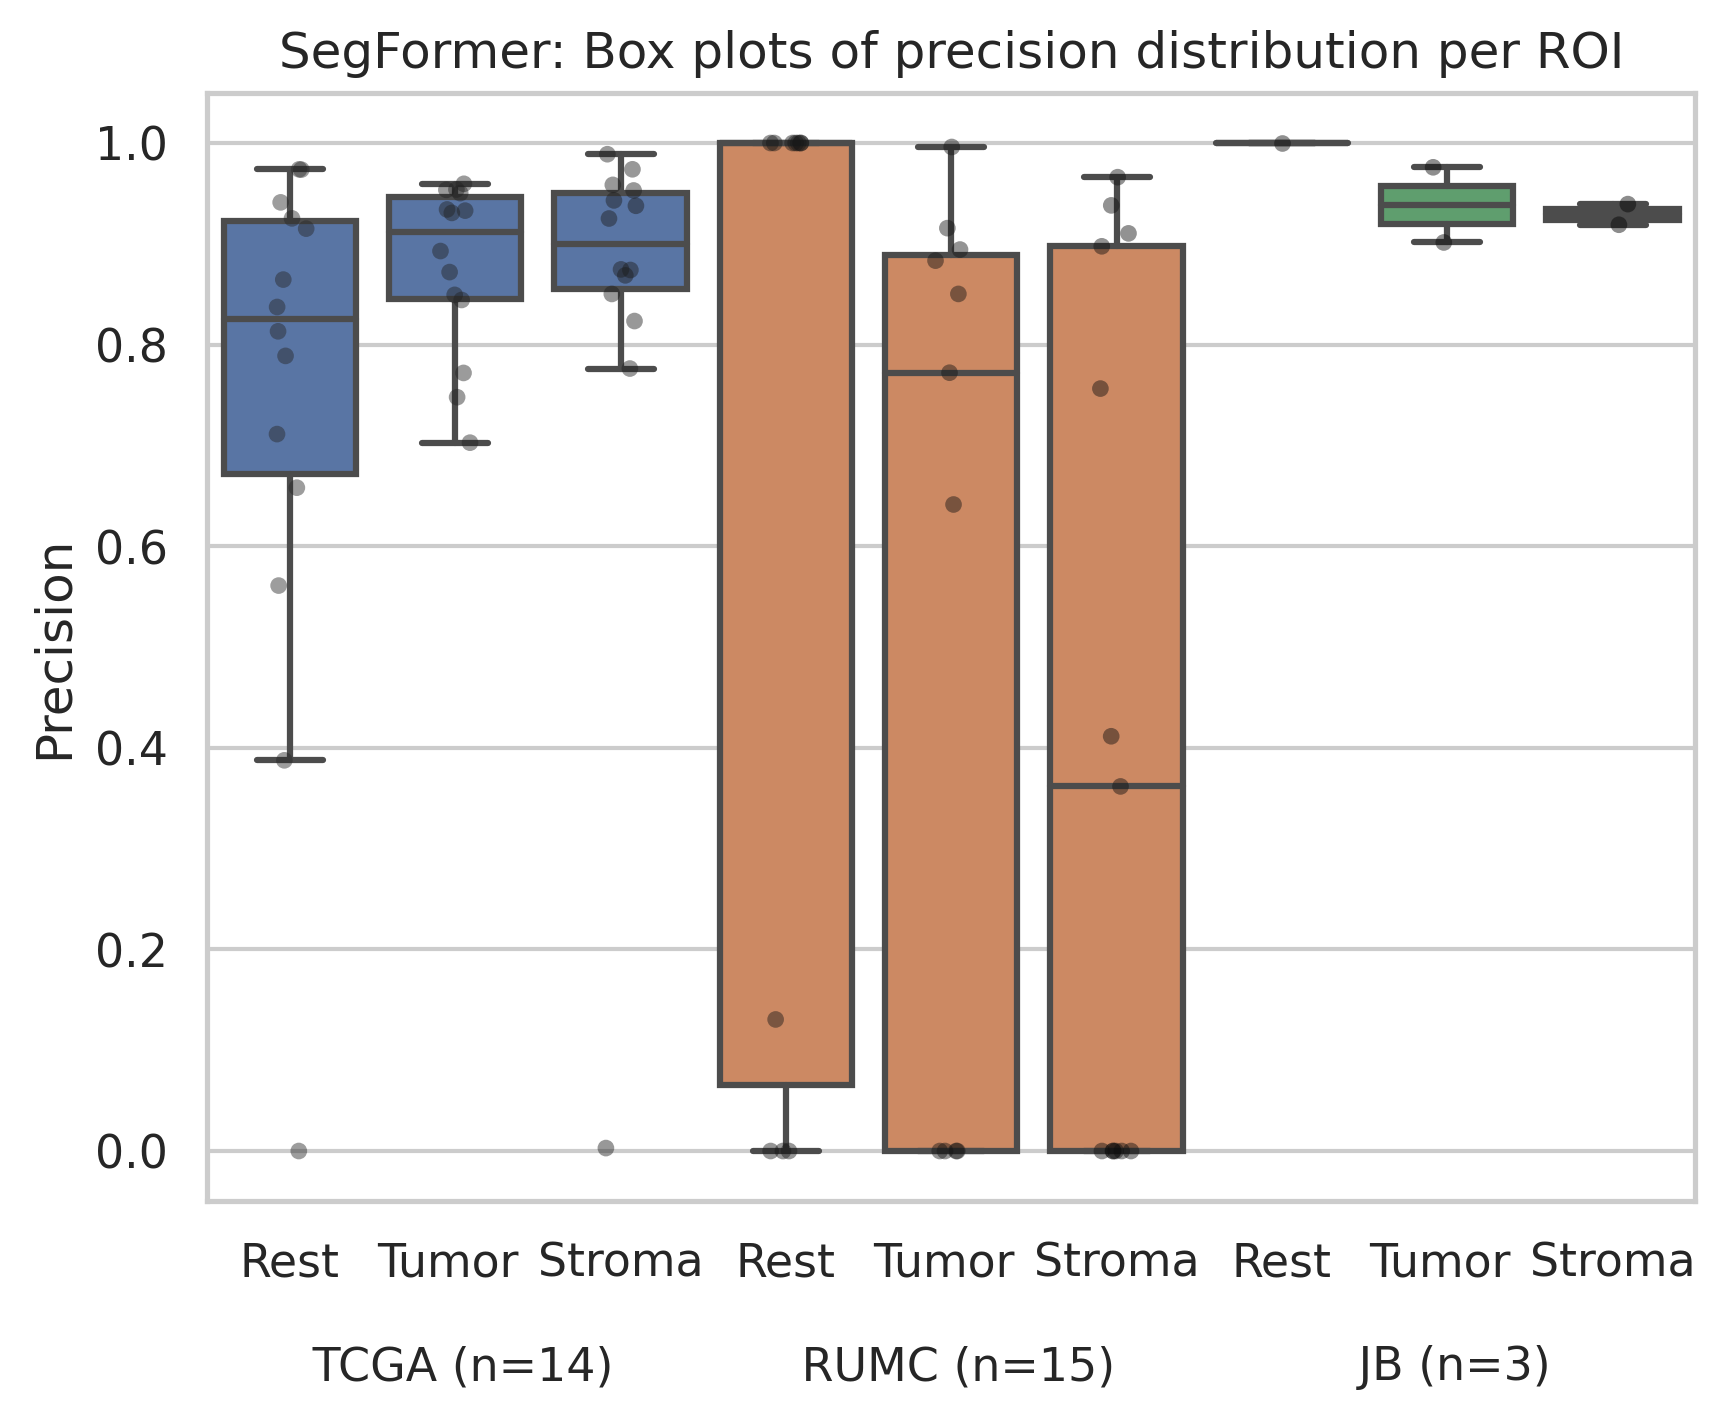
\includegraphics[width=.5\linewidth]{figures/tissue/segformer_prec_roi_wsirois.png}
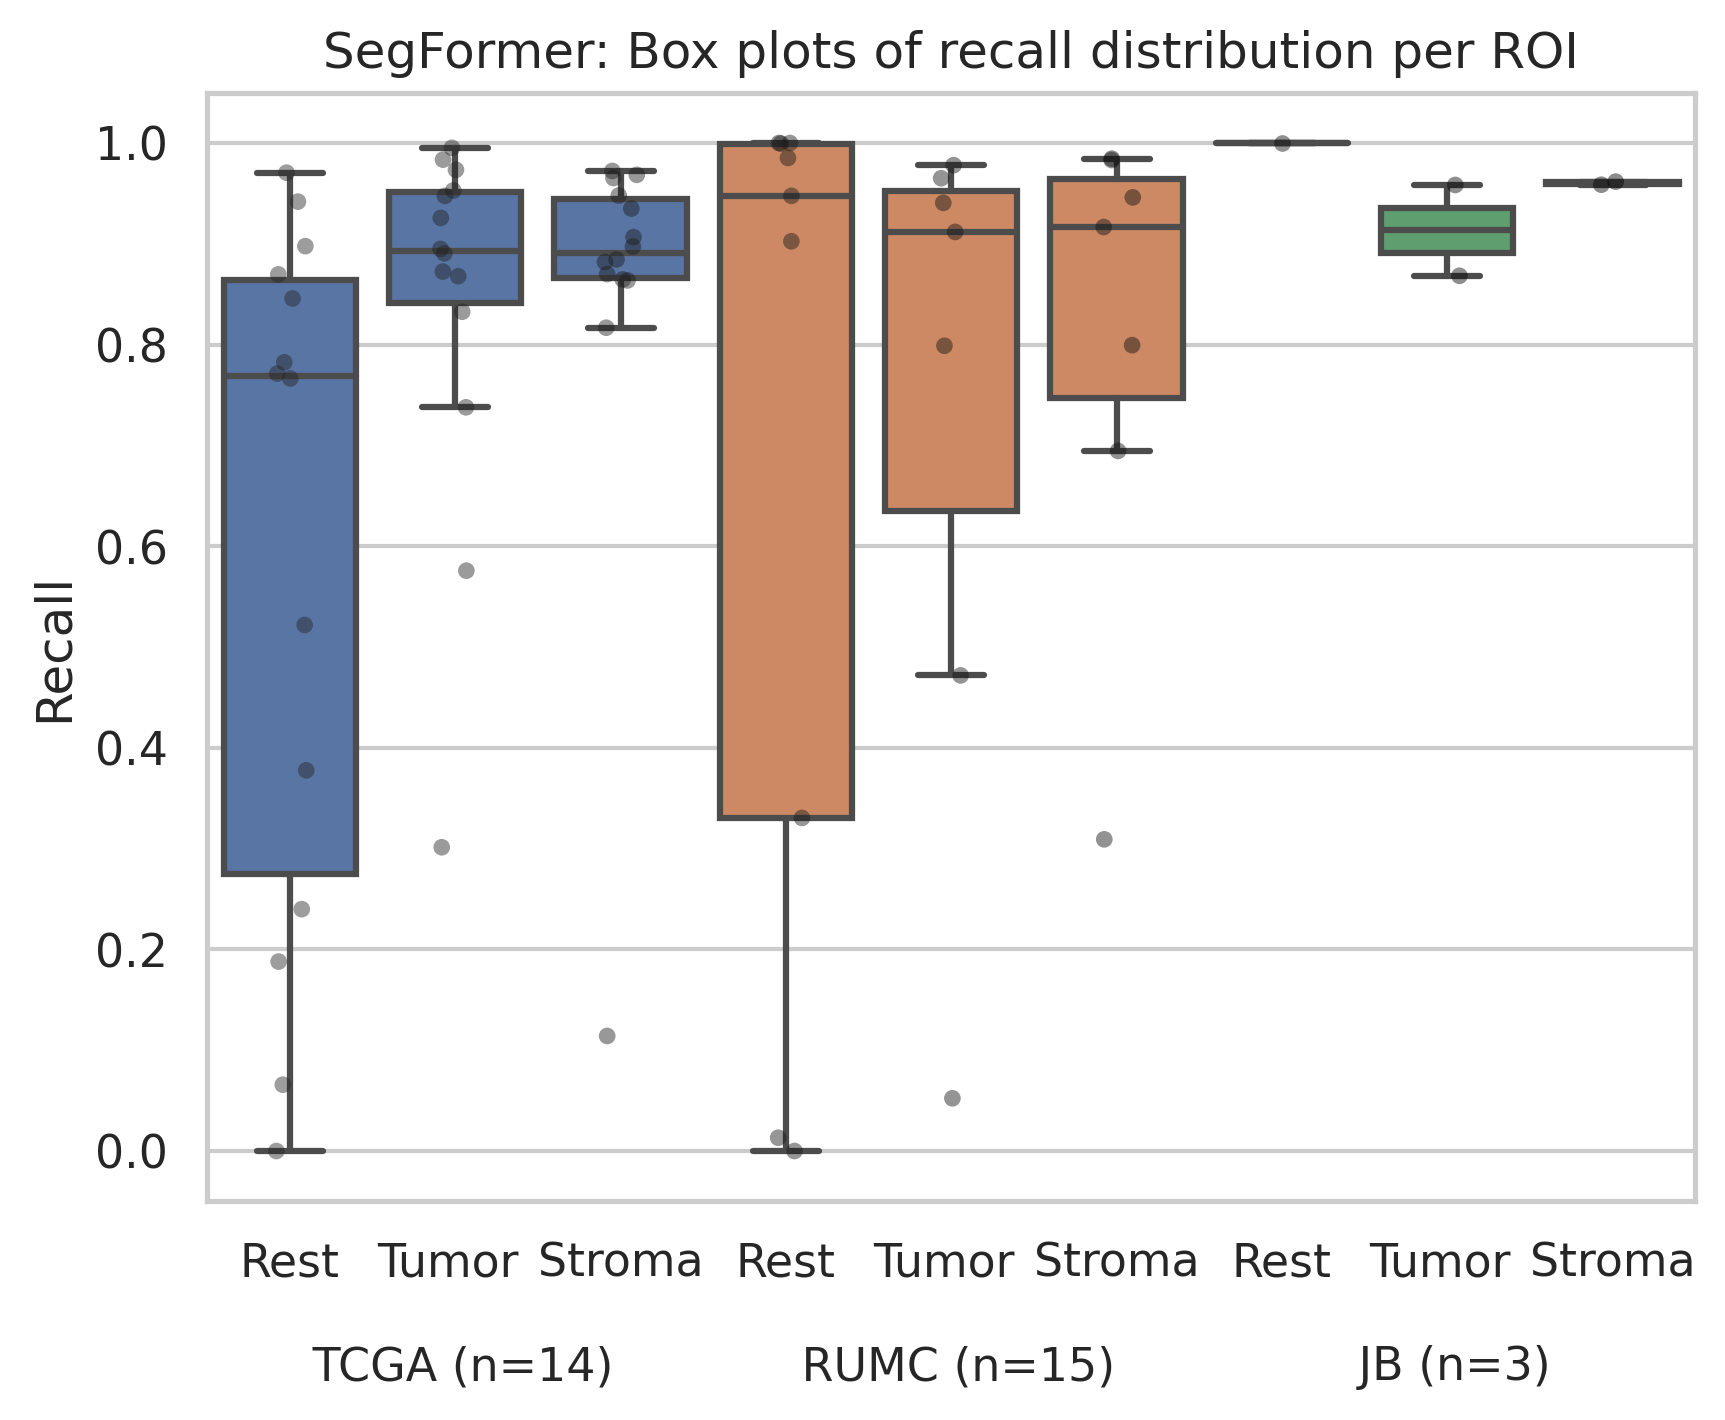
\includegraphics[width=.5\linewidth]{figures/tissue/segformer_recall_roi_wsirois.png}

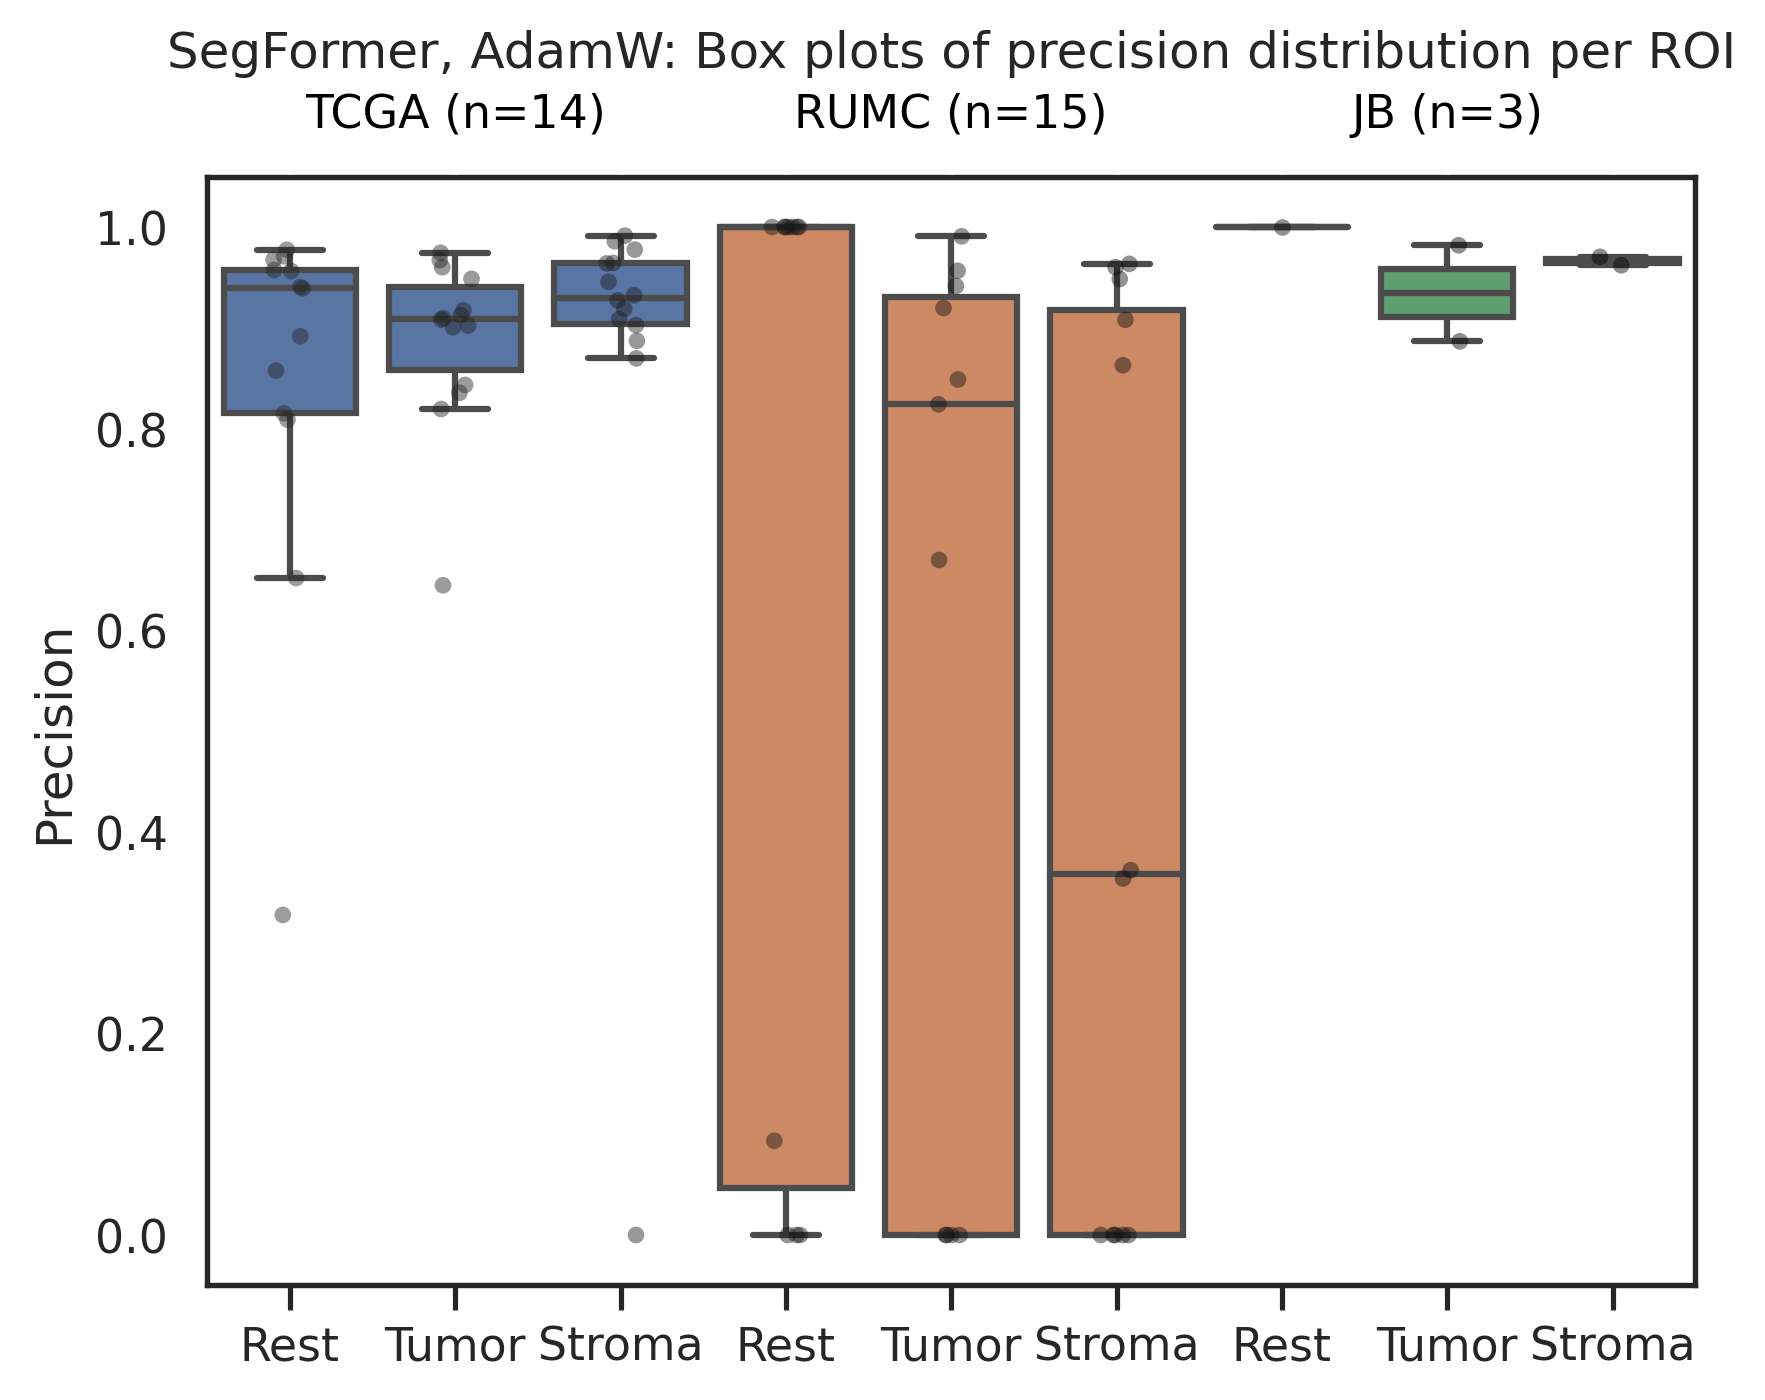
\includegraphics[width=.5\linewidth]{figures/tissue/segformer,_adamw_prec_roi_wsirois.png}
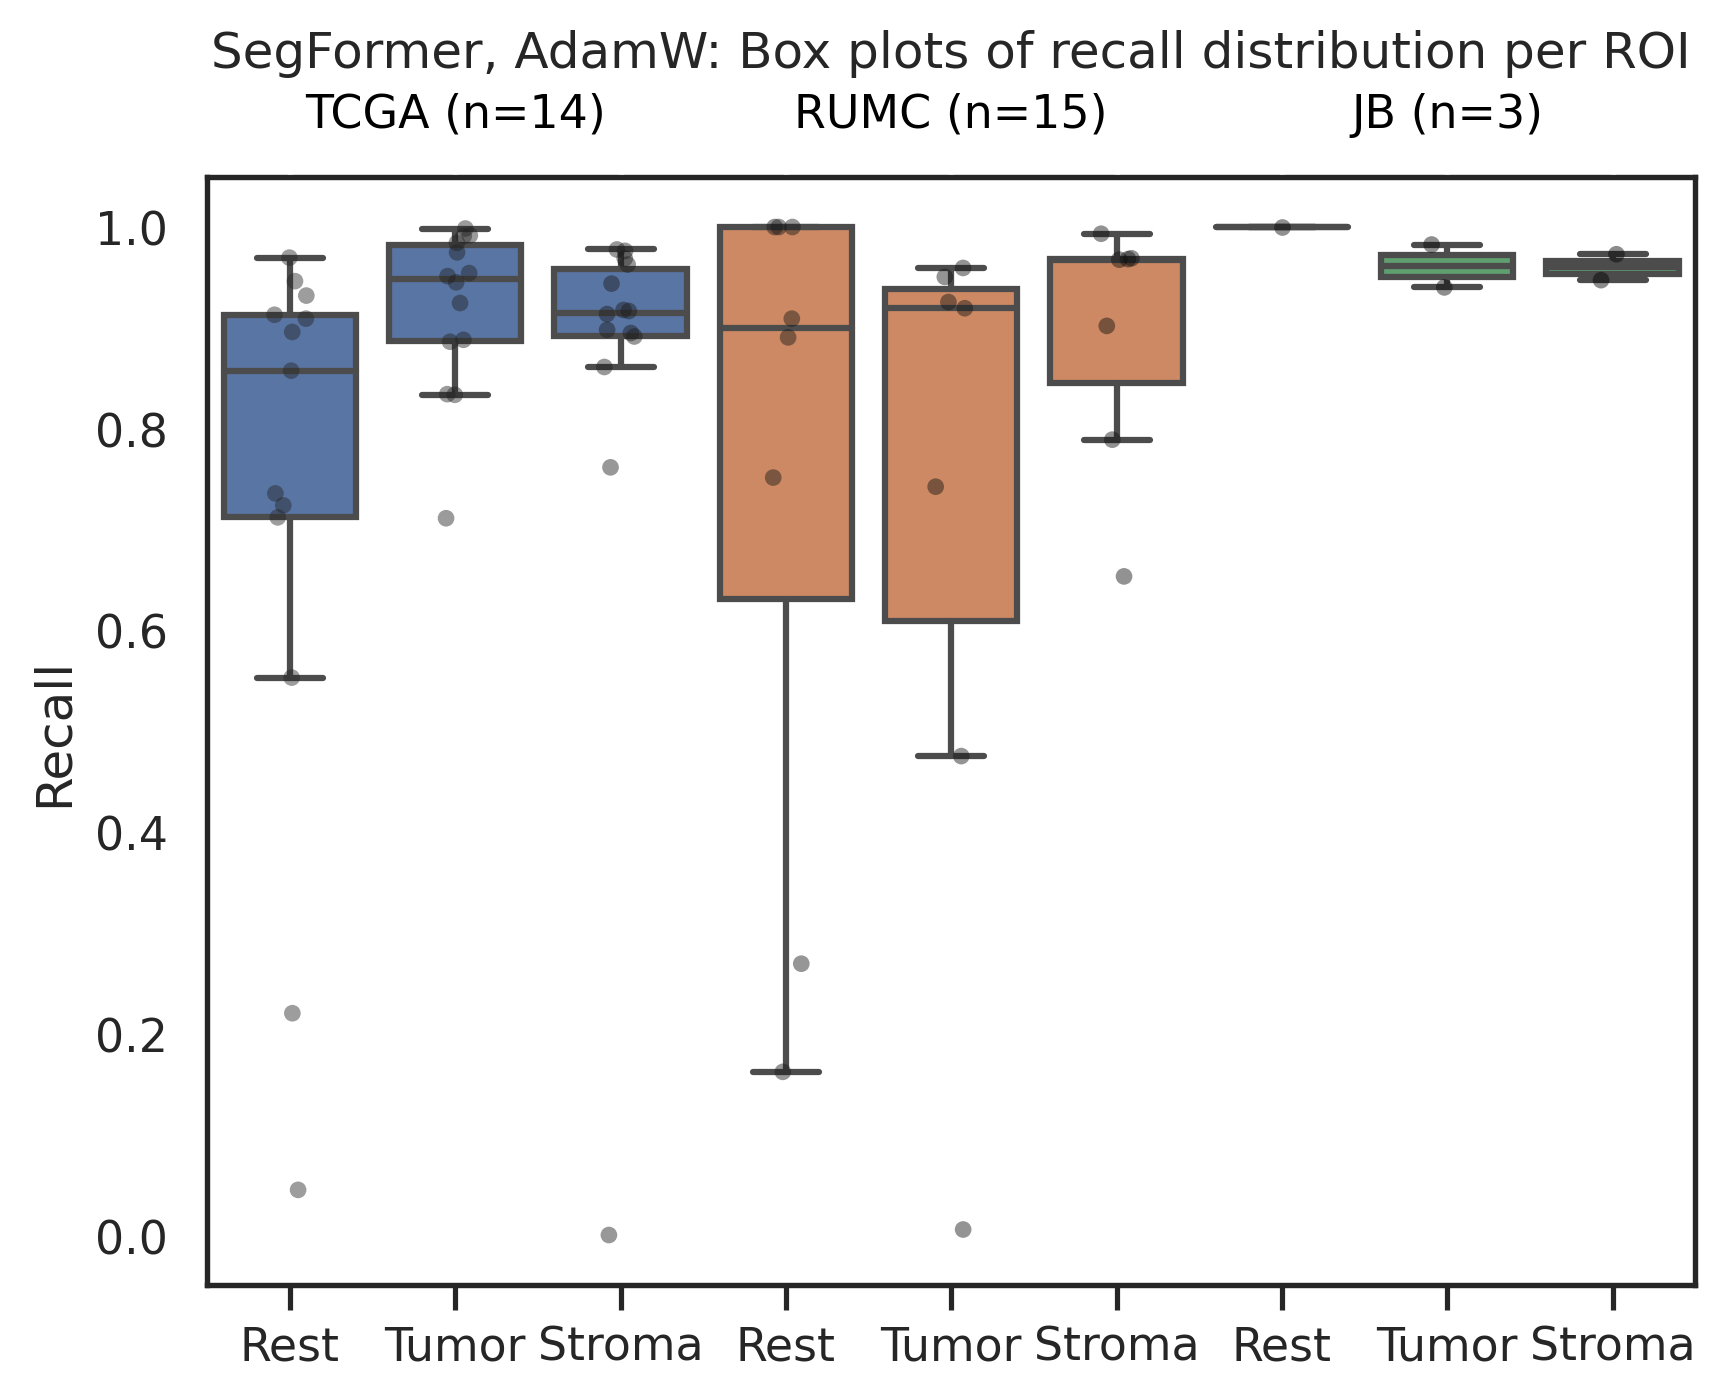
\includegraphics[width=.5\linewidth]{figures/tissue/segformer,_adamw_recall_roi_wsirois.png}
\caption{Boxplots of pixel wise calculated precision and recall across three datastes (TCGA-BRCA, RUMC, JB) and three segmentation labels.}
\label{fig:tissue_pr_r_boxplots}
\end{figure}

\begin{figure}[H]
    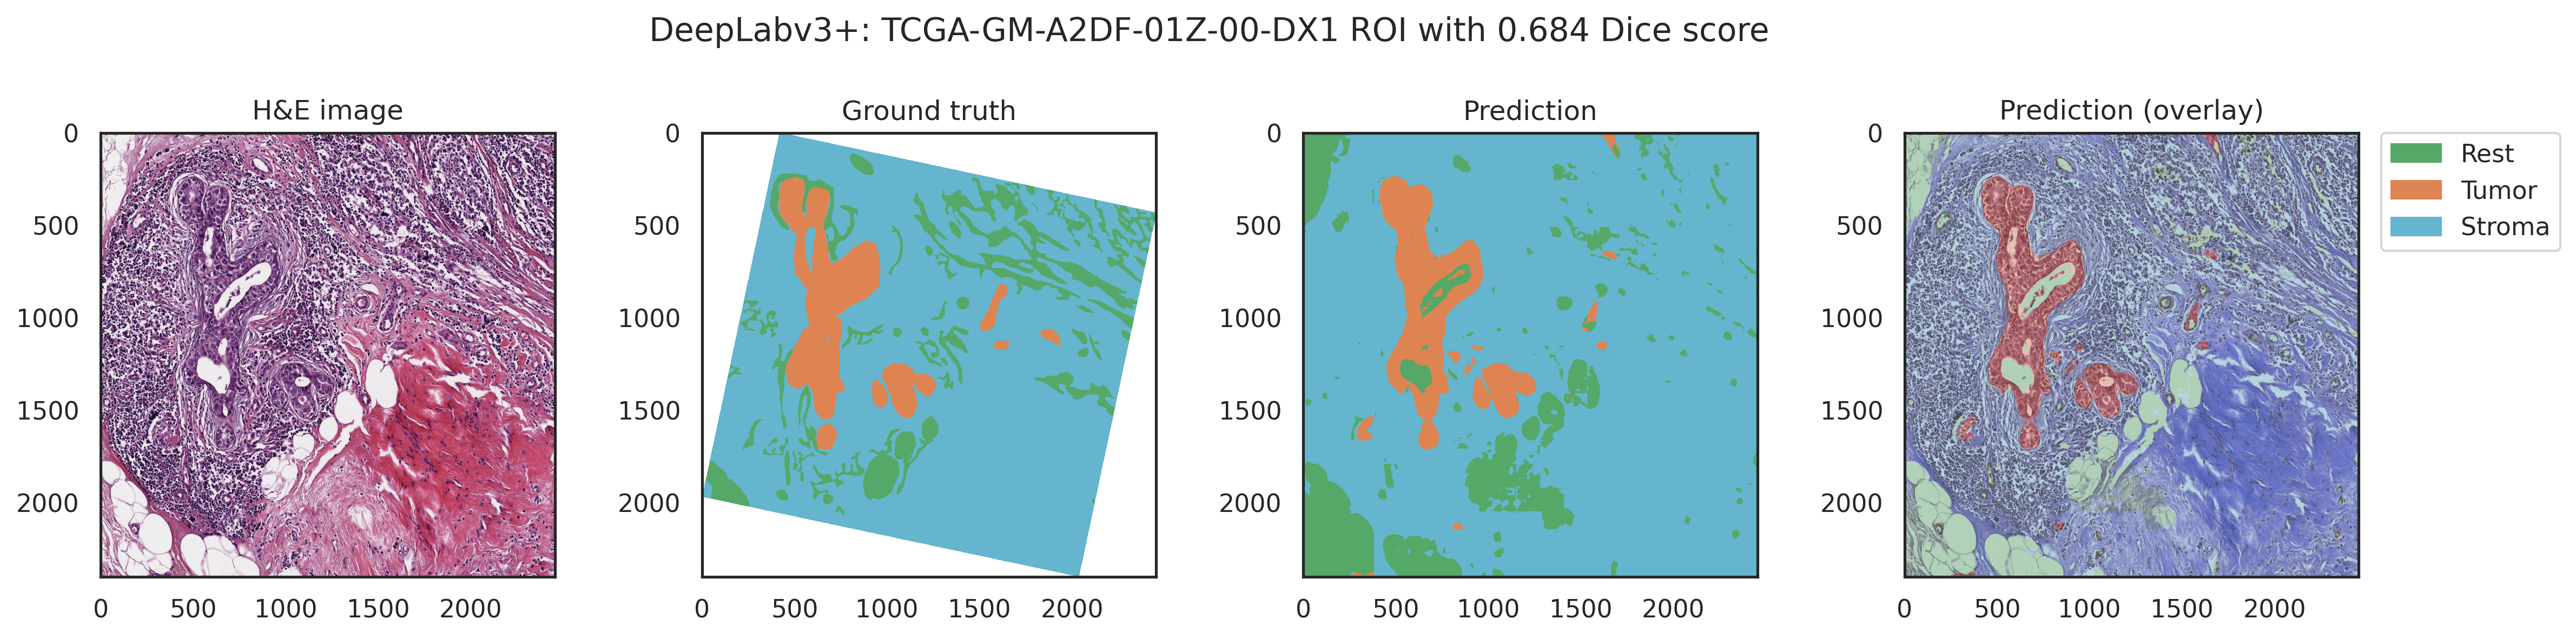
\includegraphics[width=\linewidth]{figures/tissue/deeplabv3+_dice_tcga_TCGA-GM-A2DF-01Z-00-DX1CD0BE6D7-2DB3-4193-84CC-F9BE7BF18CC2_[25322,_21890,_27778,_24293]_check.png}
    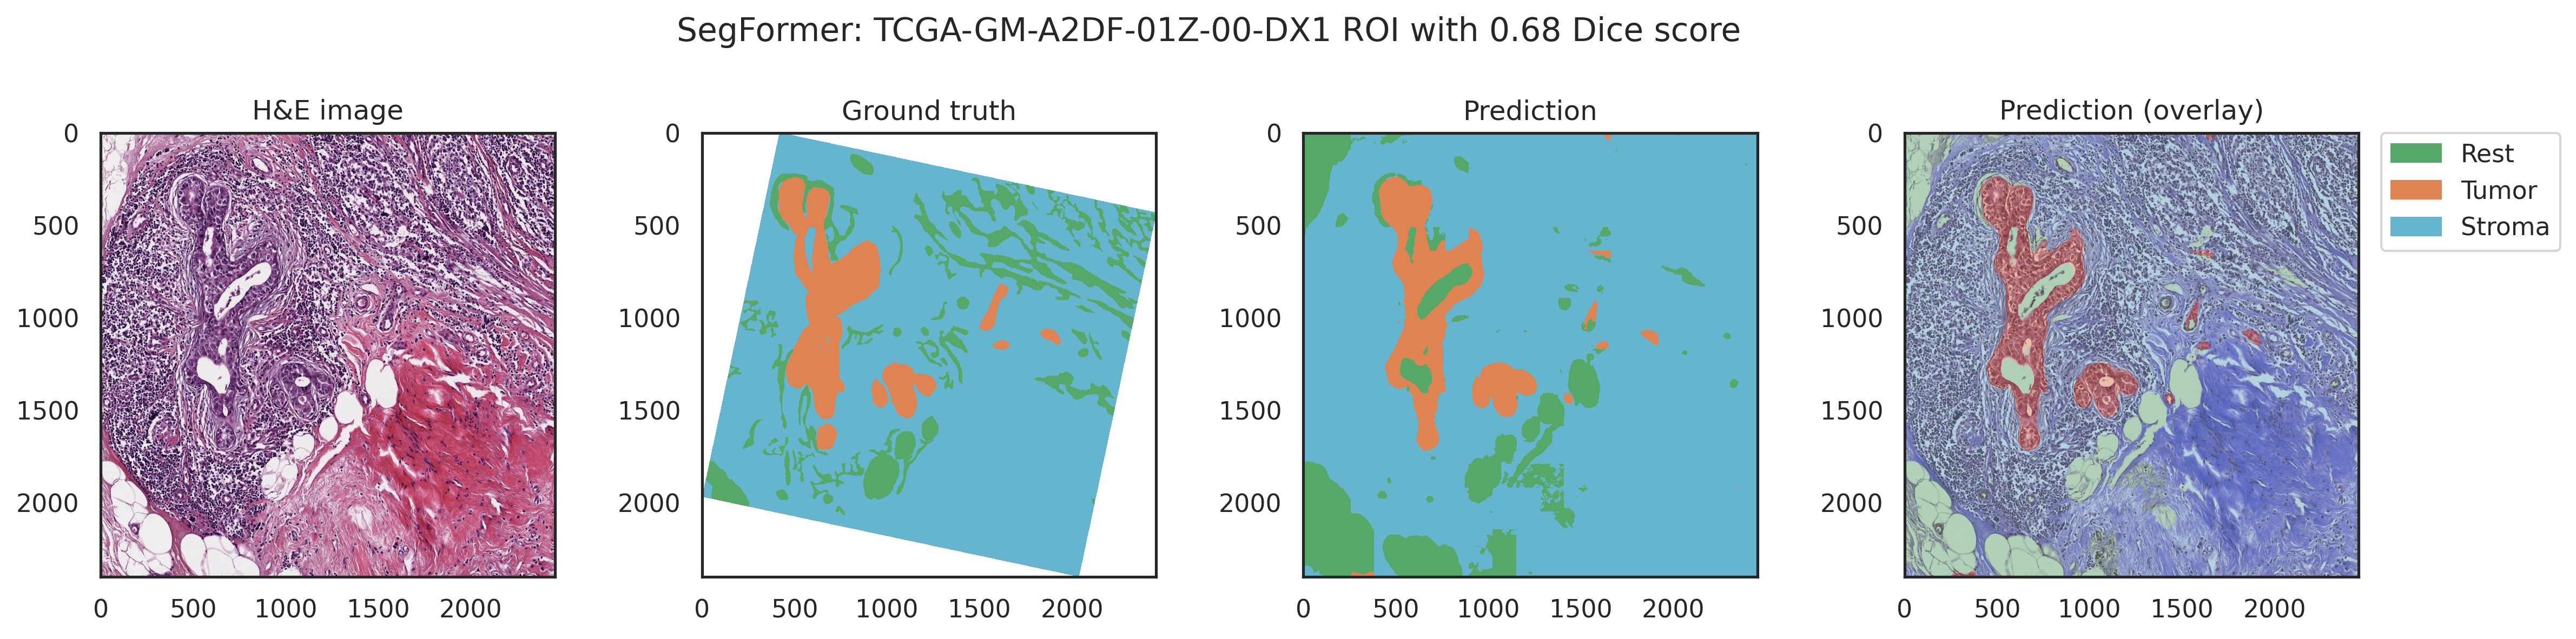
\includegraphics[width=\linewidth]{figures/tissue/segformer_dice_tcga_TCGA-GM-A2DF-01Z-00-DX1CD0BE6D7-2DB3-4193-84CC-F9BE7BF18CC2_[25322,_21890,_27778,_24293]_check.png}
    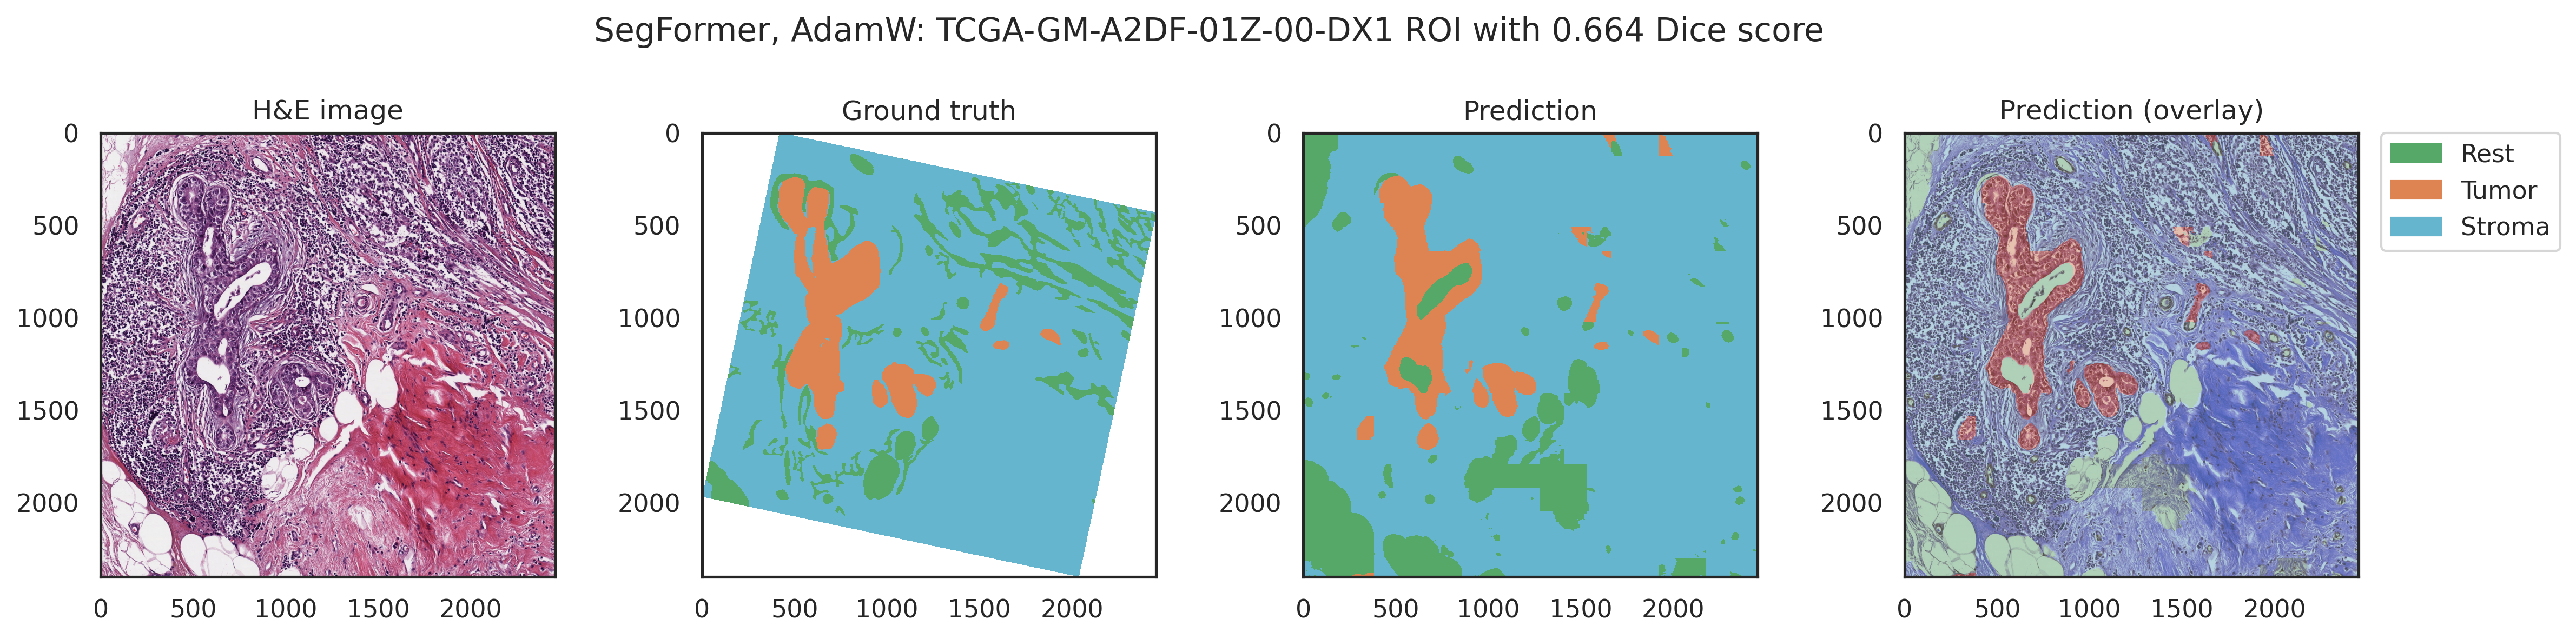
\includegraphics[width=\linewidth]{figures/tissue/segformer,_adamw_dice_tcga_TCGA-GM-A2DF-01Z-00-DX1CD0BE6D7-2DB3-4193-84CC-F9BE7BF18CC2_[25322,_21890,_27778,_24293]_check.png}
    
    \caption{Example of a slightly devalued dice score due to some annotation inaccuracies.}
    \label{fig:TCGA-GM-A2DF}
\end{figure}
    

\begin{figure}[H]
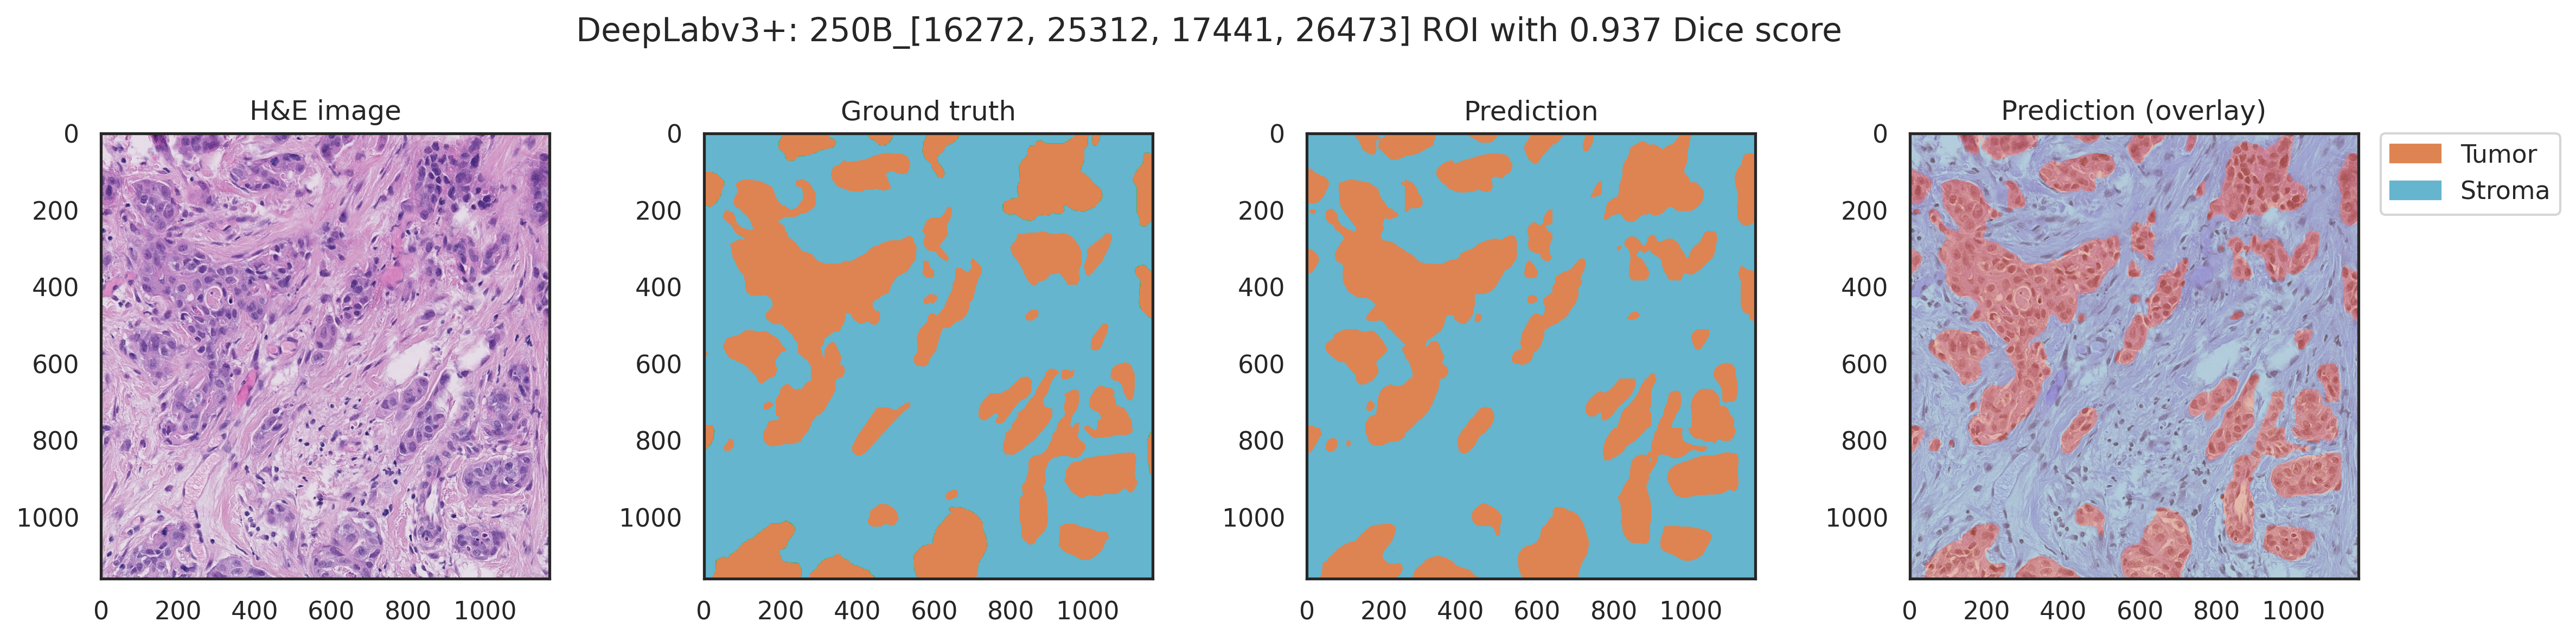
\includegraphics[width=\linewidth]{figures/tissue/deeplabv3+_dice_s_250B_[16272,_25312,_17441,_26473]_check.png}
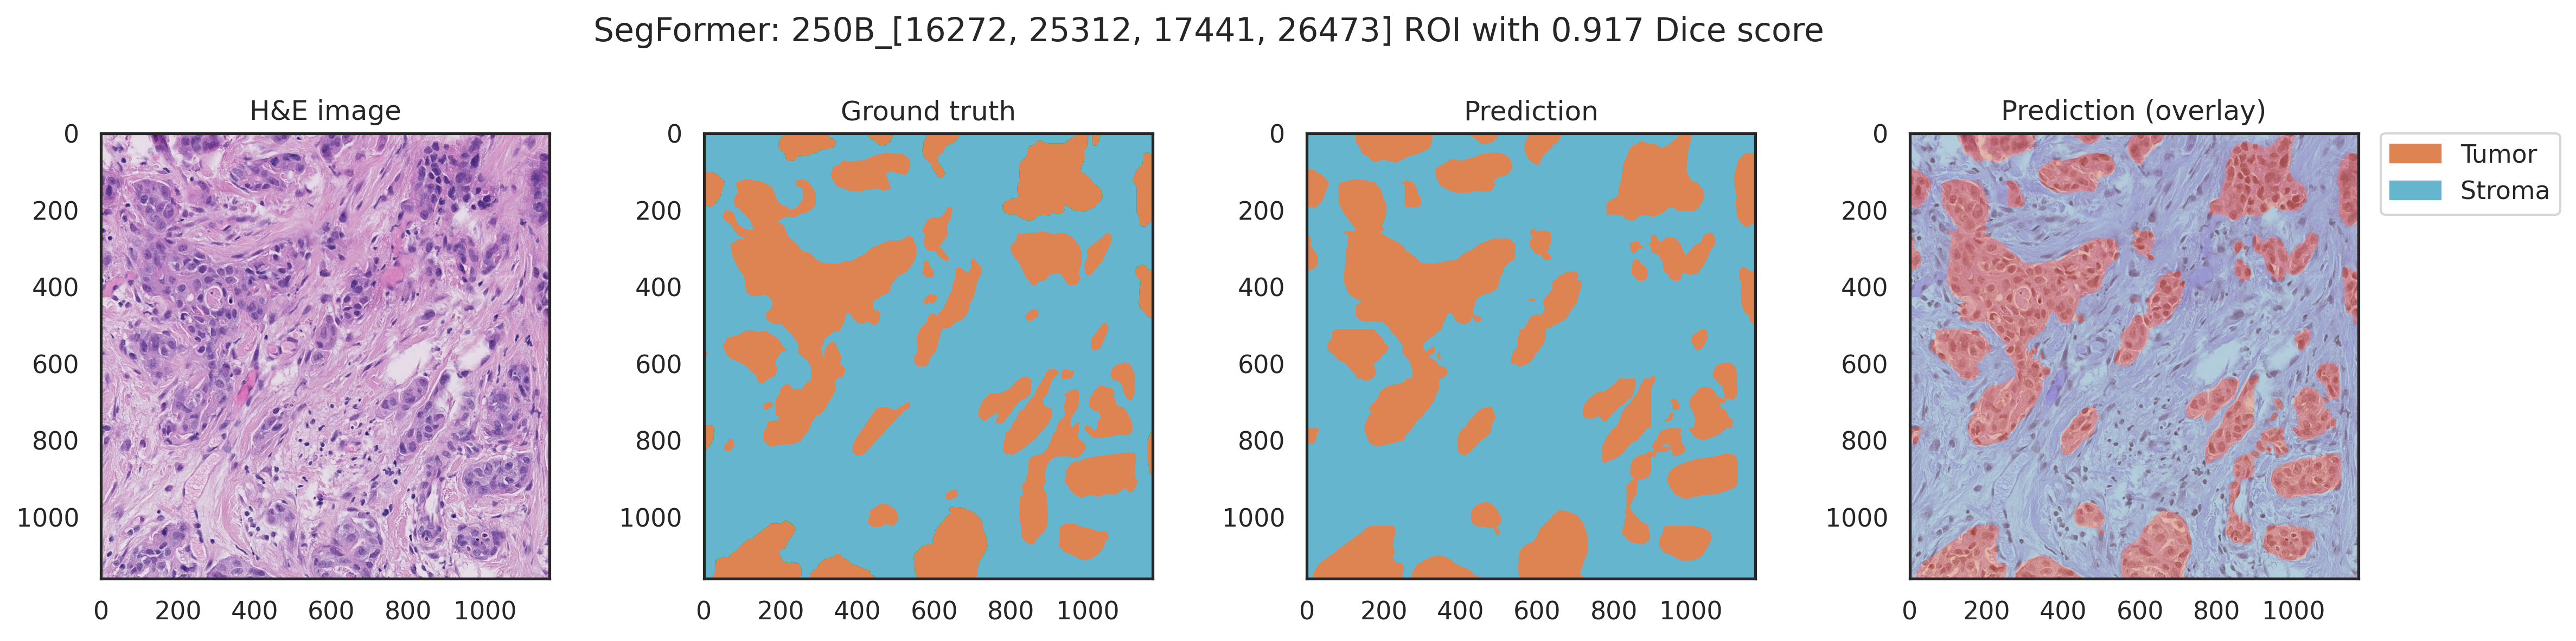
\includegraphics[width=\linewidth]{figures/tissue/segformer_dice_s_250B_[16272,_25312,_17441,_26473]_check.png}
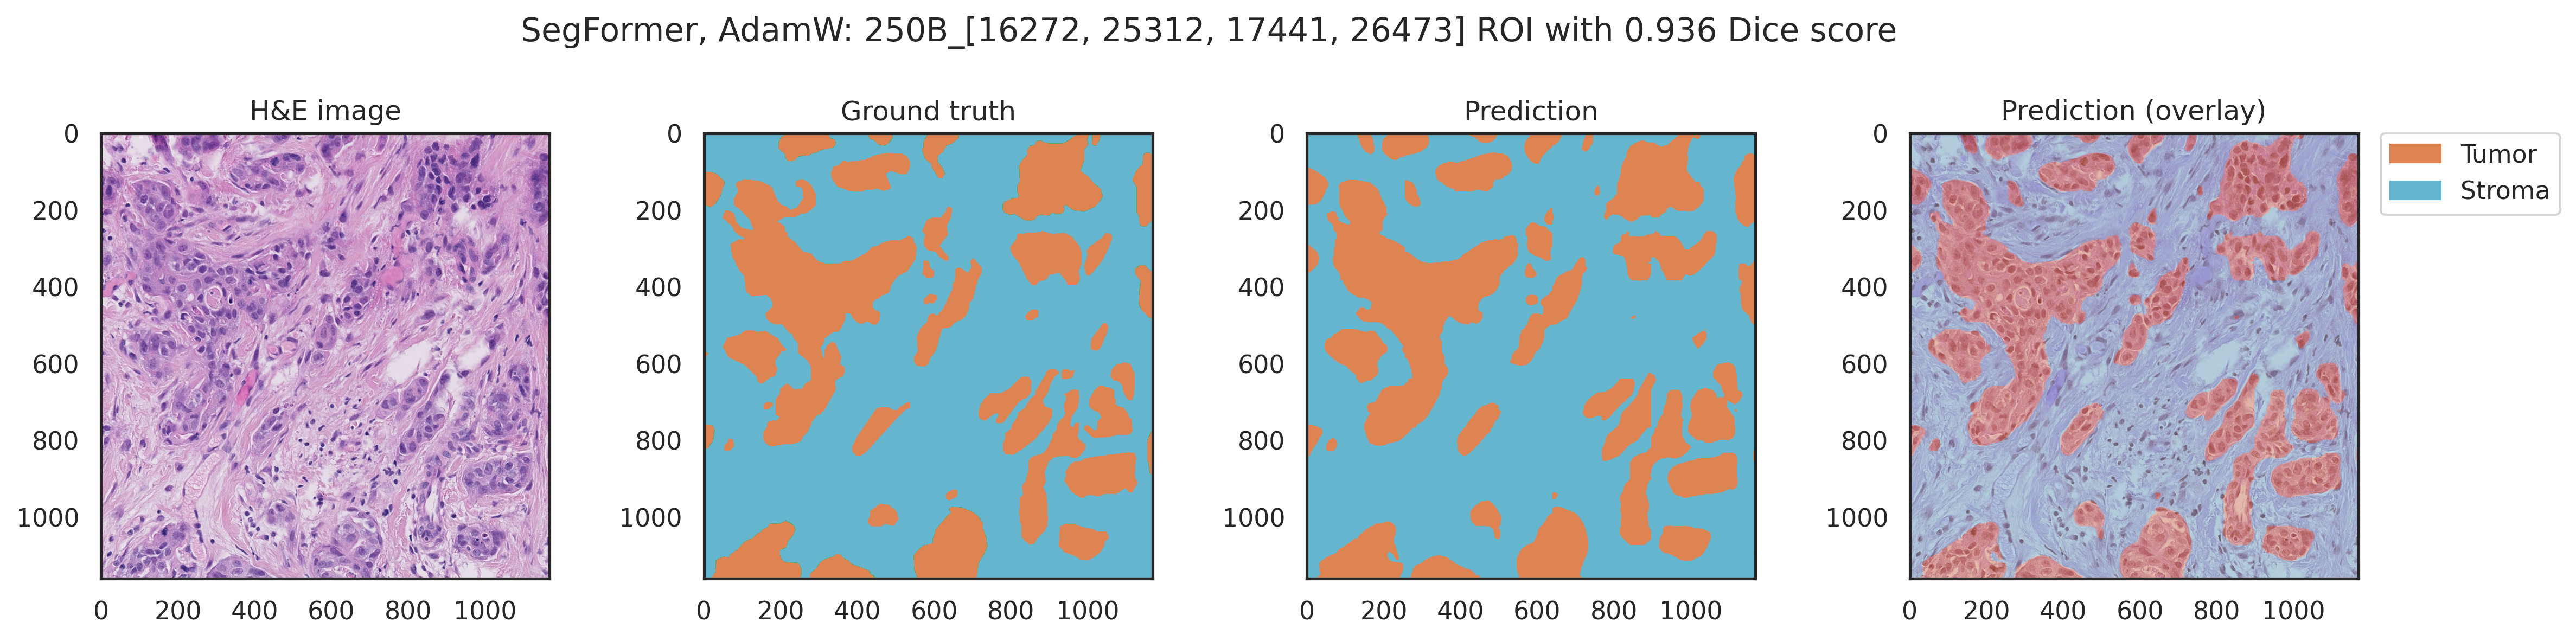
\includegraphics[width=\linewidth]{figures/tissue/segformer,_adamw_dice_s_250B_[16272,_25312,_17441,_26473]_check.png}

\caption{JB S\_250B ROI segmentation result.}
\label{fig:s_250B_1}
\end{figure}

\begin{figure}[H]
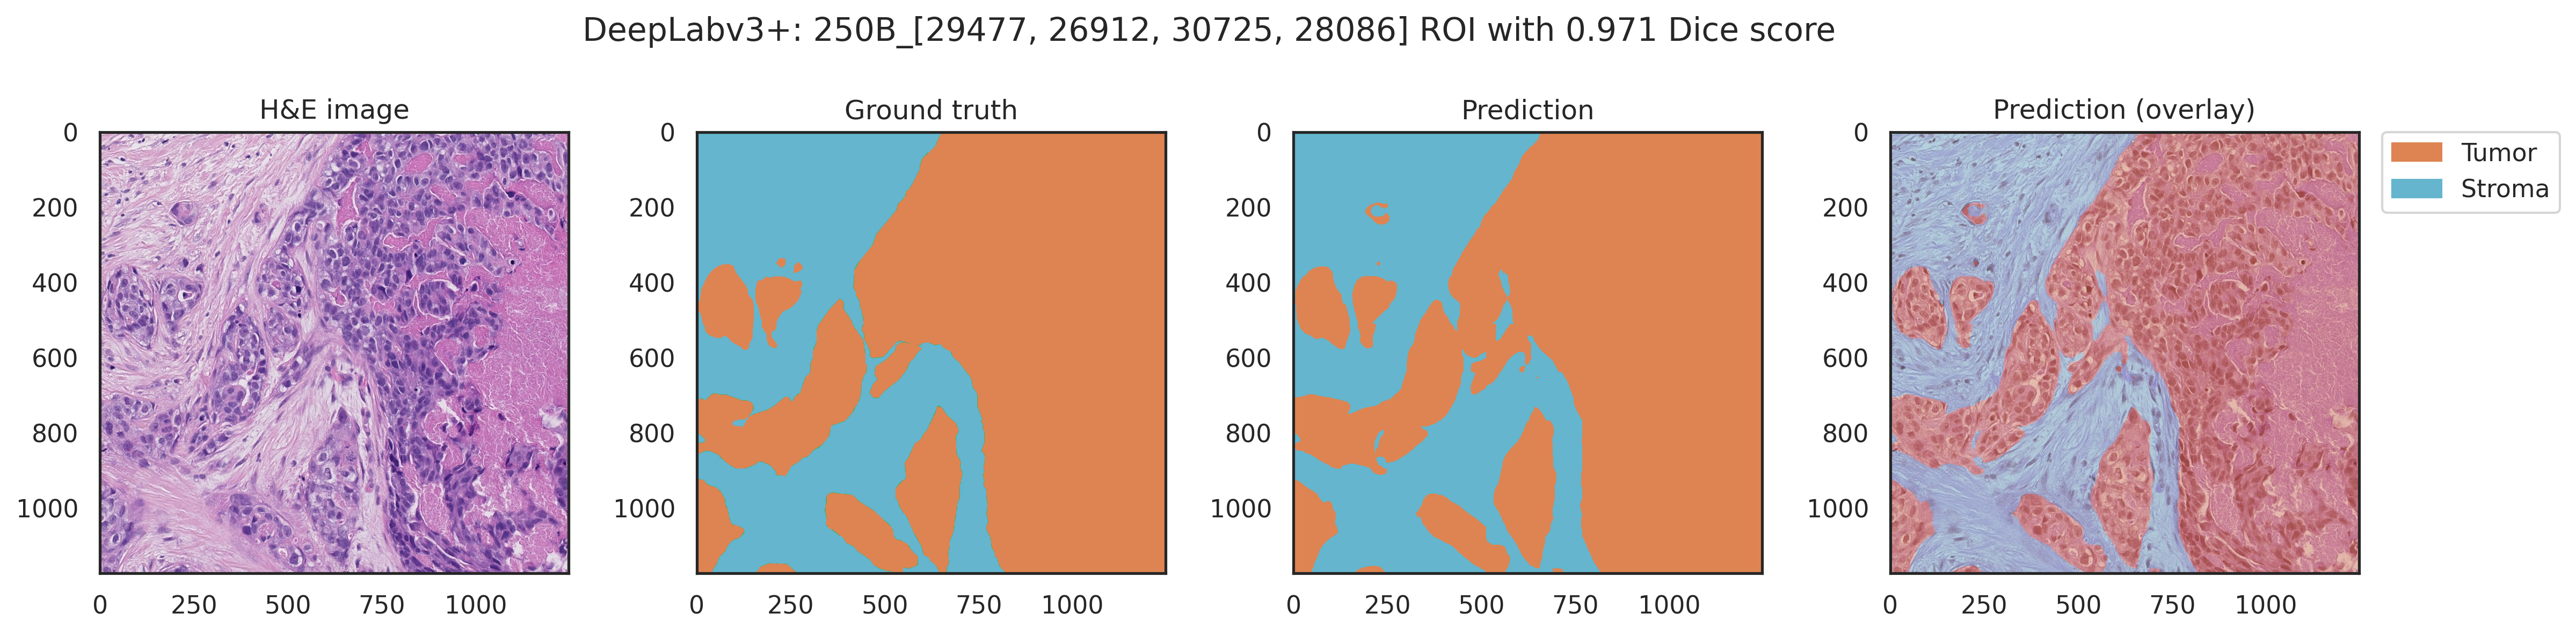
\includegraphics[width=\linewidth]{figures/tissue/deeplabv3+_dice_s_250B_[29477,_26912,_30725,_28086]_check.png}
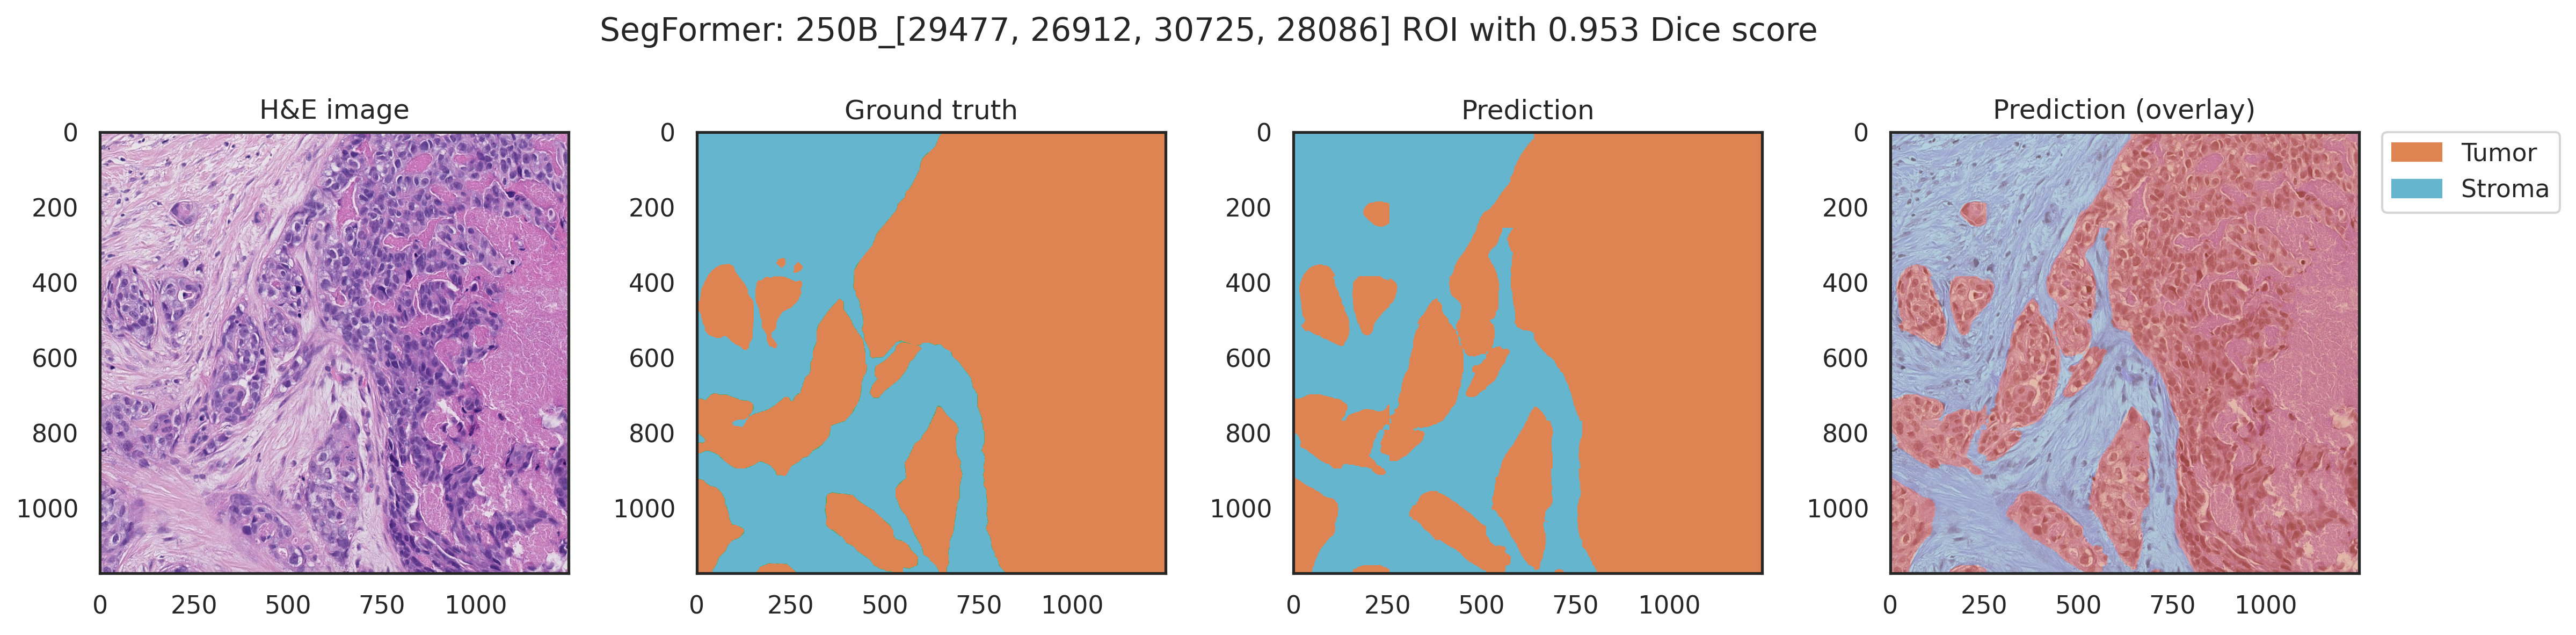
\includegraphics[width=\linewidth]{figures/tissue/segformer_dice_s_250B_[29477,_26912,_30725,_28086]_check.png}
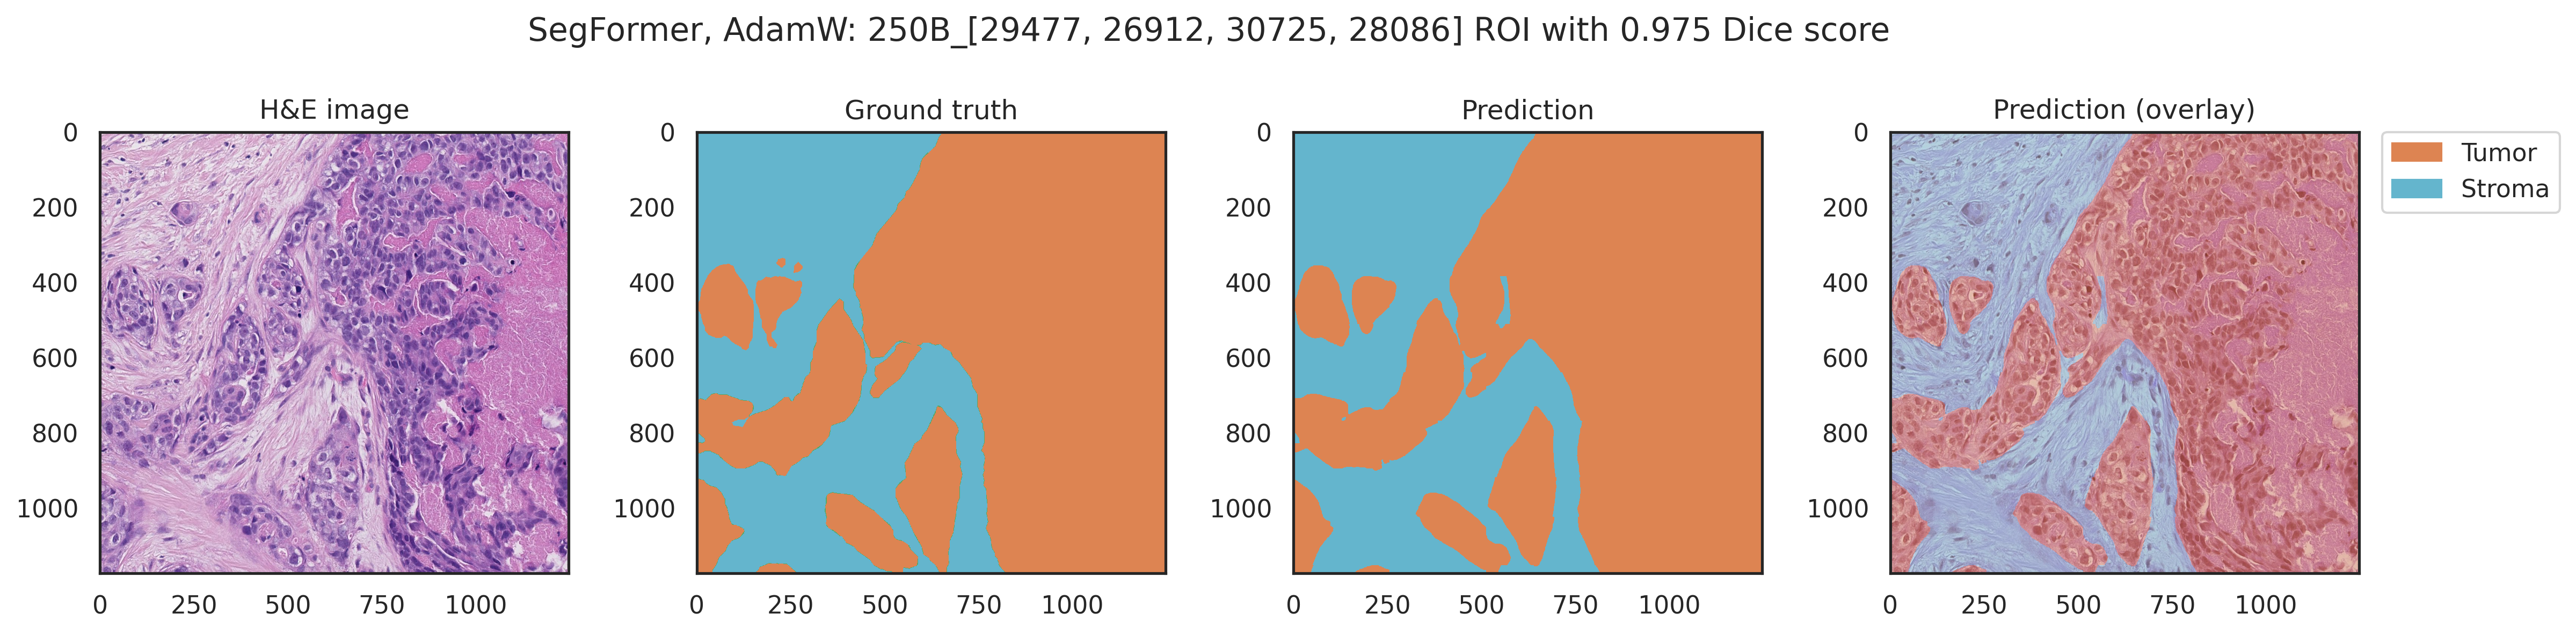
\includegraphics[width=\linewidth]{figures/tissue/segformer,_adamw_dice_s_250B_[29477,_26912,_30725,_28086]_check.png}

\caption{JB S\_250B ROI segmentation result.}
\label{fig:s_250B_2}
\end{figure}

\begin{figure}[H]
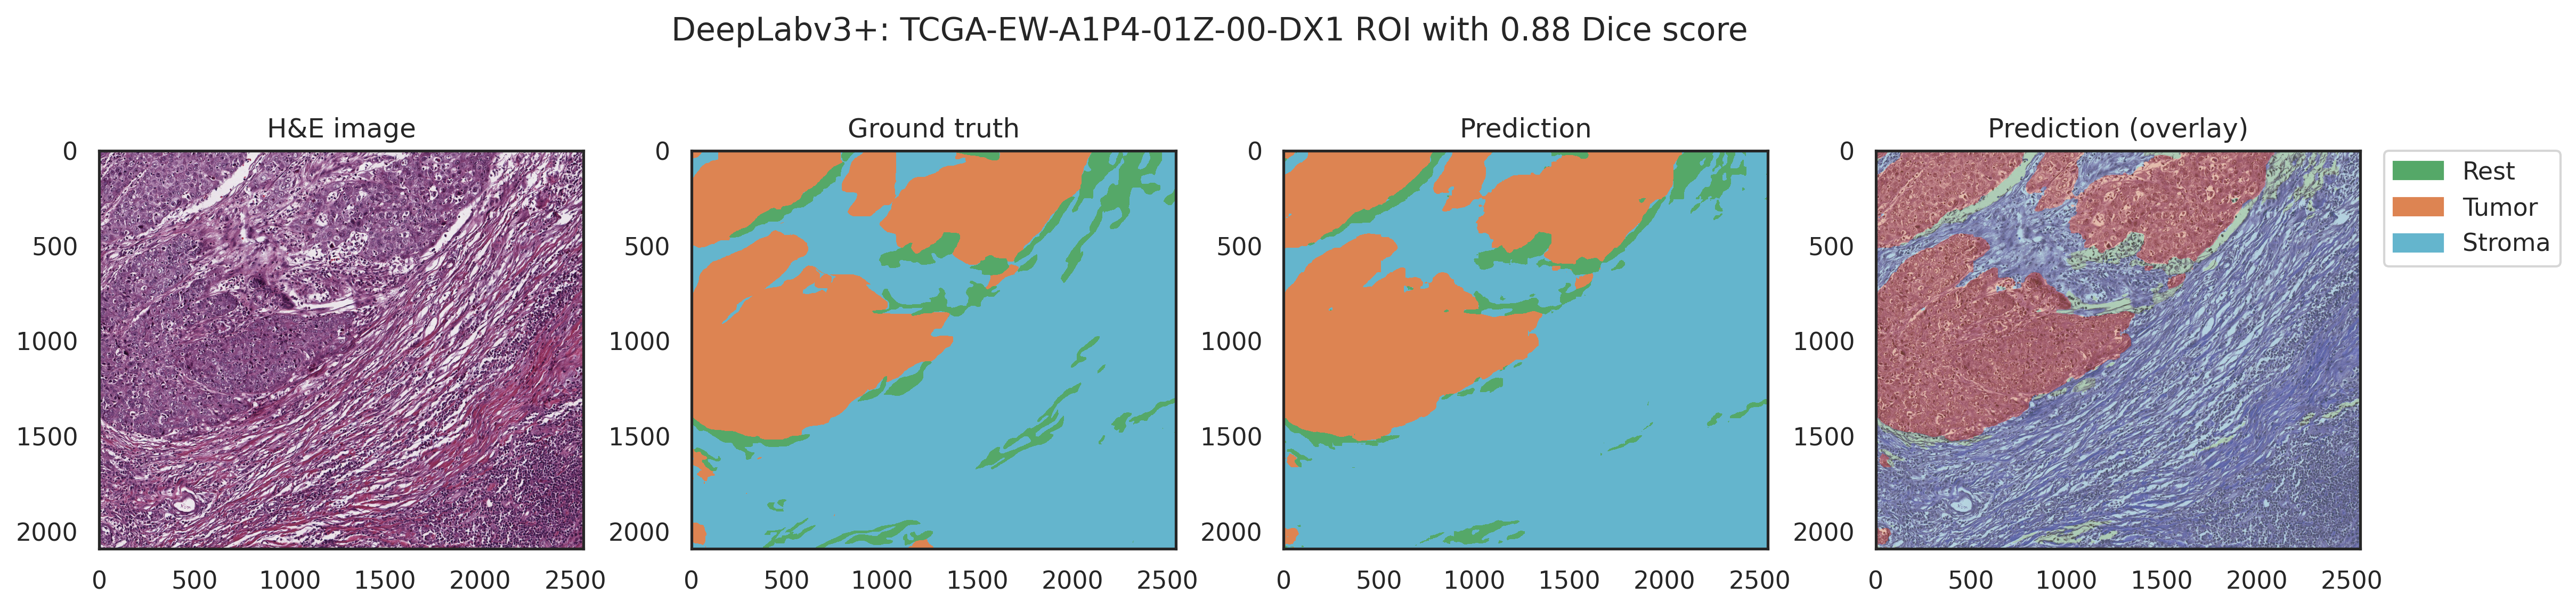
\includegraphics[width=\linewidth]{figures/tissue/deeplabv3+_dice_tcga_TCGA-EW-A1P4-01Z-00-DX13E9AE553-83D4-4B09-AB7F-D096BCE3BC4D_[8630,_17717,_11173,_19809]_check.png}
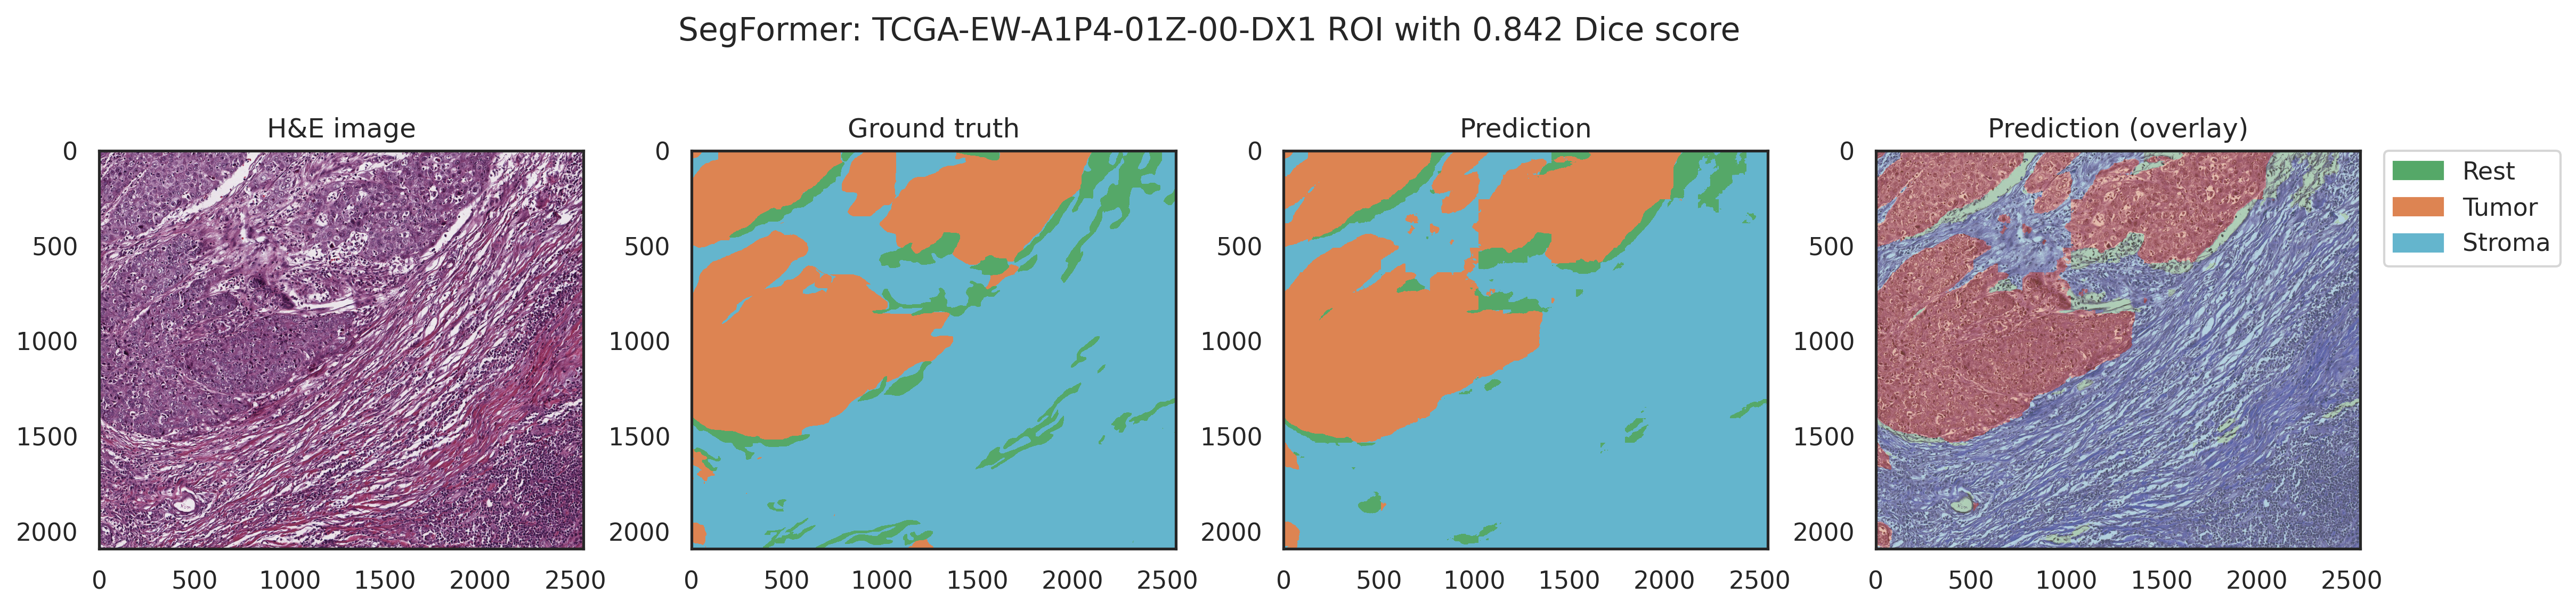
\includegraphics[width=\linewidth]{figures/tissue/segformer_dice_tcga_TCGA-EW-A1P4-01Z-00-DX13E9AE553-83D4-4B09-AB7F-D096BCE3BC4D_[8630,_17717,_11173,_19809]_check.png}
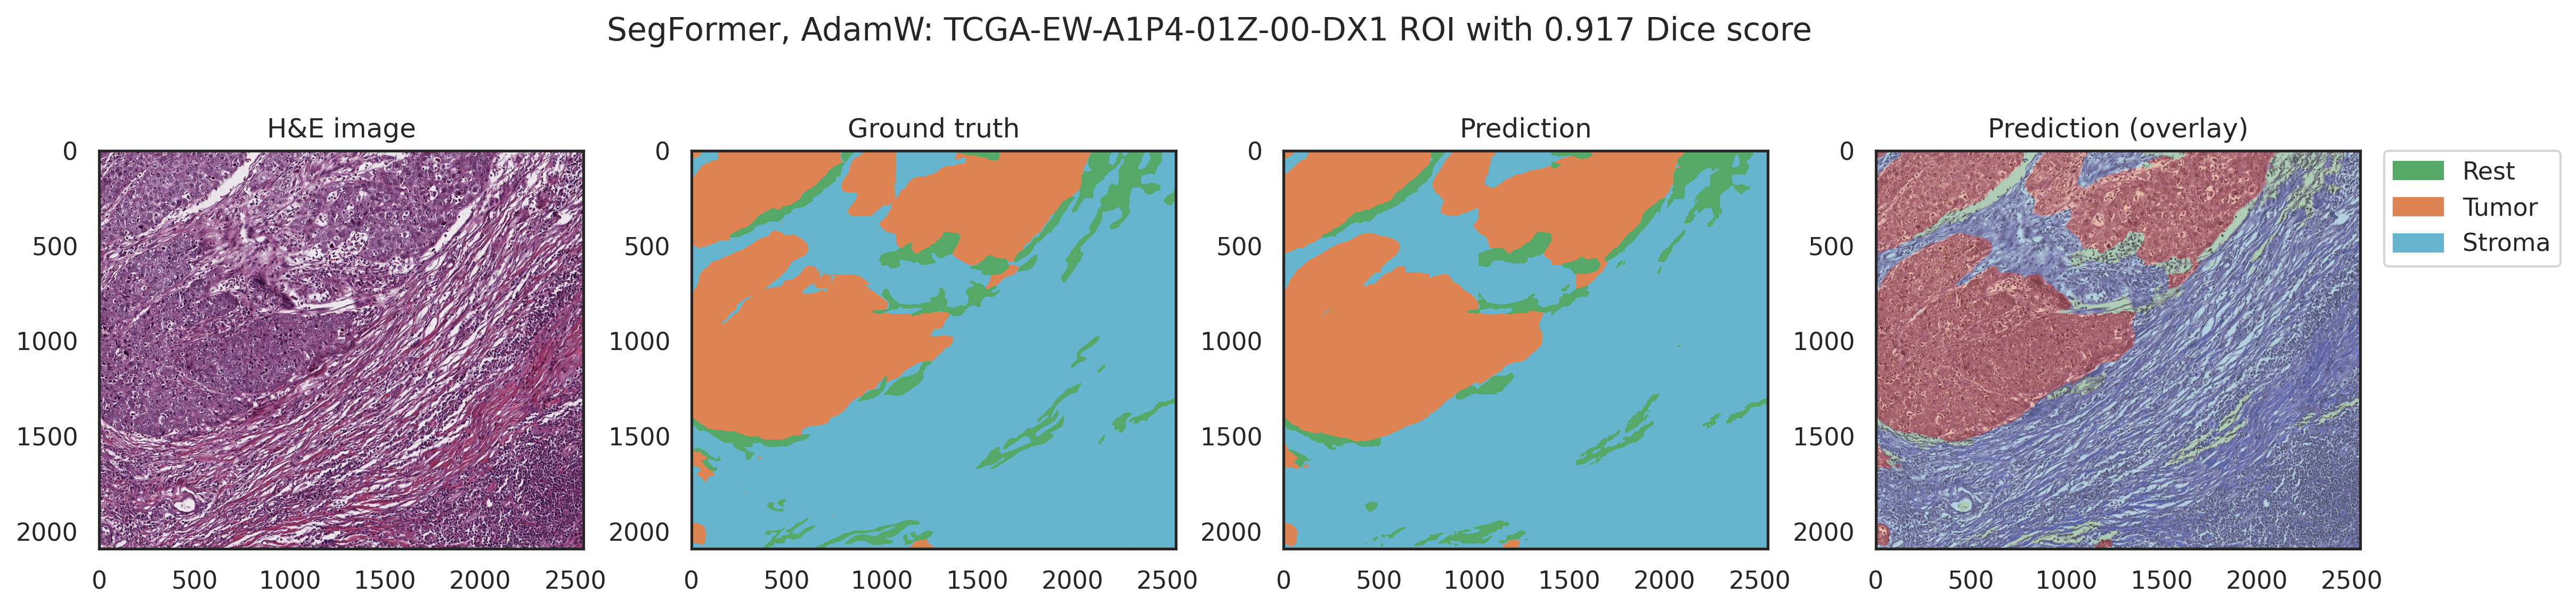
\includegraphics[width=\linewidth]{figures/tissue/segformer,_adamw_dice_tcga_TCGA-EW-A1P4-01Z-00-DX13E9AE553-83D4-4B09-AB7F-D096BCE3BC4D_[8630,_17717,_11173,_19809]_check.png}

\caption{TCGA-EW-A1P4-01Z-00-DX1 ROI segmentation result.}
\label{fig:TCGA-EW-A1P4}
\end{figure}



\section{TILs Segmentation}
TILs segmentation task aimed to segment the RGB input of H\&E stained image at 20$\times$ magnification
(resolution of 0.5 micron-per-pixel) into two prediction maps: TILs and rest.
The split of the patients was used similarly to the previously described in
Tabel~\ref*{tab:patients_sep}. Even though the same patients are present in
this data set, the annotations originate from a different
study which results in a different ROI and patch statistics shown in
Table~\ref*{tab:patch_sep_tils}. The patches were created using a sliding
window approach with 128$\times$128 sized patches
and stride equals 100. The ROIs that were smaller than 128$\times$128
were padded. The additional rotation augmentation was applied,
by rotating each patch 5 times at 9 degrees each.
The column "Number of patches that include rest" in Table~\ref*{tab:patch_sep_tils}
seems excessive, but was still added
for better data comprehension: the ROIs for TILs segmentation are either
completely annotated as rest or include occasional TILs masks.
%This unequal distribution of the classes cause the dataset to be imbalanced.

\begin{table}[h!]
    \centering
    \begin{tabular}{ l c c c c c c c }
        \hline
        & \multirow{2}{*}{slides} & \multirow{2}{*}{ROIs}& \multirow{2}{*}{patches}& \multicolumn{4}{c}{Number of patches that include}\\ 
        \cline{5-8}
        & & & & TILs & Rest & 1 class & 2 classes \\
        \hline
        Train & 156 & 1\,552 & 106\,974 & 35\,433 & 106\,974 & 71\,541 & 35\,433\\
         &  &  &  & (33\%) & (100\%) & (67\%) & (33\%)  \\
        Validation & 20 & 154 & 15\,518 & 14\,164 & 15\,518 & 5\,638 & 3\,734 \\
         &  &  &  & (27\%) & (100\%) & (60\%) & (40\%)\\
        Test & 19 & 173 & 9\,372 & 3\,734 & 9\,372& 11\,354 & 4\,164\\
         &  &  &  & (40\%) & (100\%) & (73\%) & (27\%)\\
        \hline
        & 195 & 1\,879 & 131\,864 &  &  &  & \\
    \end{tabular}
    \caption{\label{tab:patch_sep_tils} Overview of patches that were split into train, validation,
    and test sets for TILs segmentation. The percentages indicate the fraction of a specific conditioned
    group of patches to the number of all patches in the "patches" column.}
\end{table}

The model architectures and their parameters were used as described in~\ref*{res_tissue_segm}:
DeepLabv3+, SegFormer with Adam optimizer, and SegFormer with AdamW. An important
change is an increased batch size of 128, which was allowed due to smaller patch
sizes of 128$\times$128. In the model overview in Table~\ref*{tab:tils_perform}
the number of parameters and
iterations remain the same. FLOPs values are dependent on input shape, therefore
it was expected to drop since the input is smaller.
It is aslo noticed that for TILs segmentation the runtime between all three models
becomes comparable in contrast to tissue segmentation (Table~\ref*{tab:tissue_perform}).

\begin{table}[h!]
    \centering
    \begin{tabular}{ l c c c c c c c c}
        \hline
        Model & FLOPs & Params & Iterations & Runtime & F1 score & Precision & Recall\\
        \hline
        DeepLabv3+ & 11.04 & 43.58 M & 160 K & 2d 8h 36m & 0.49 & 0.58 & 0.43\\
        SegFormer & 3.24 & 81.97 M & 160 K  & 2d 11h 36m & 0.62 & 0.62 & 0.33\\
        SegFormer, & \multirow{2}{*}{3.24} & \multirow{2}{*}{81.97 M} & \multirow{2}{*}{160 K} & \multirow{2}{*}{2d 15h 19m} & \multirow{2}{*}{\textbf{0.66}} & \multirow{2}{*}{0.64} & \multirow{2}{*}{0.69}\\
        AdamW & & & & & & & & \\
        \hline
    \end{tabular}
\caption{\label{tab:tils_perform} Overview of the trained TILs segmentation models. The runtime is given for a training on one GPU NVIDIA A100 SXM4.}
\end{table}

For proper evaluation the predicted TILs segmentation needed to be reduced to TILs
centers (one pixel) that can be then further matched to ground truth.
To get optimal centers of predicted TILs, non-maximum suppression was applied on
posterior images that were clipped between 0 and 255. The search for the best-fitted
parameter of kappa (threshold) and kernel size was completed on the validation set.
As pictured in Figure~\ref*{fig:kappas} there were multiple experiments performed
with kernel sizes  in [1, 3, 5, 7, 9, 11, 13] and multiple kappas. The highest value of
kappa was the median value over all posteriors. The consecutive values were the
two power fractions of the median. Figure~\ref*{fig:kappas} includes two images
for DeepLabv3+ (first in the first row and first in the second row) to provide a
zoomed look of the tighter range. As a result, the best parameters on the validation
set were chosen as kappa=21, kernel size=9 for DeepLabv3+ and kappa=64, kernel size=5
for SegFormer-based methods. The resulting centers were matched to
the ground truth by applying the Hungarian algorithm that found the best assignment
to match ground truth TILs with predicted ones. The allowed maximum distance for a
match of predicted with ground truth TILs was set to 5 \textmu m.

\begin{figure}[h!]
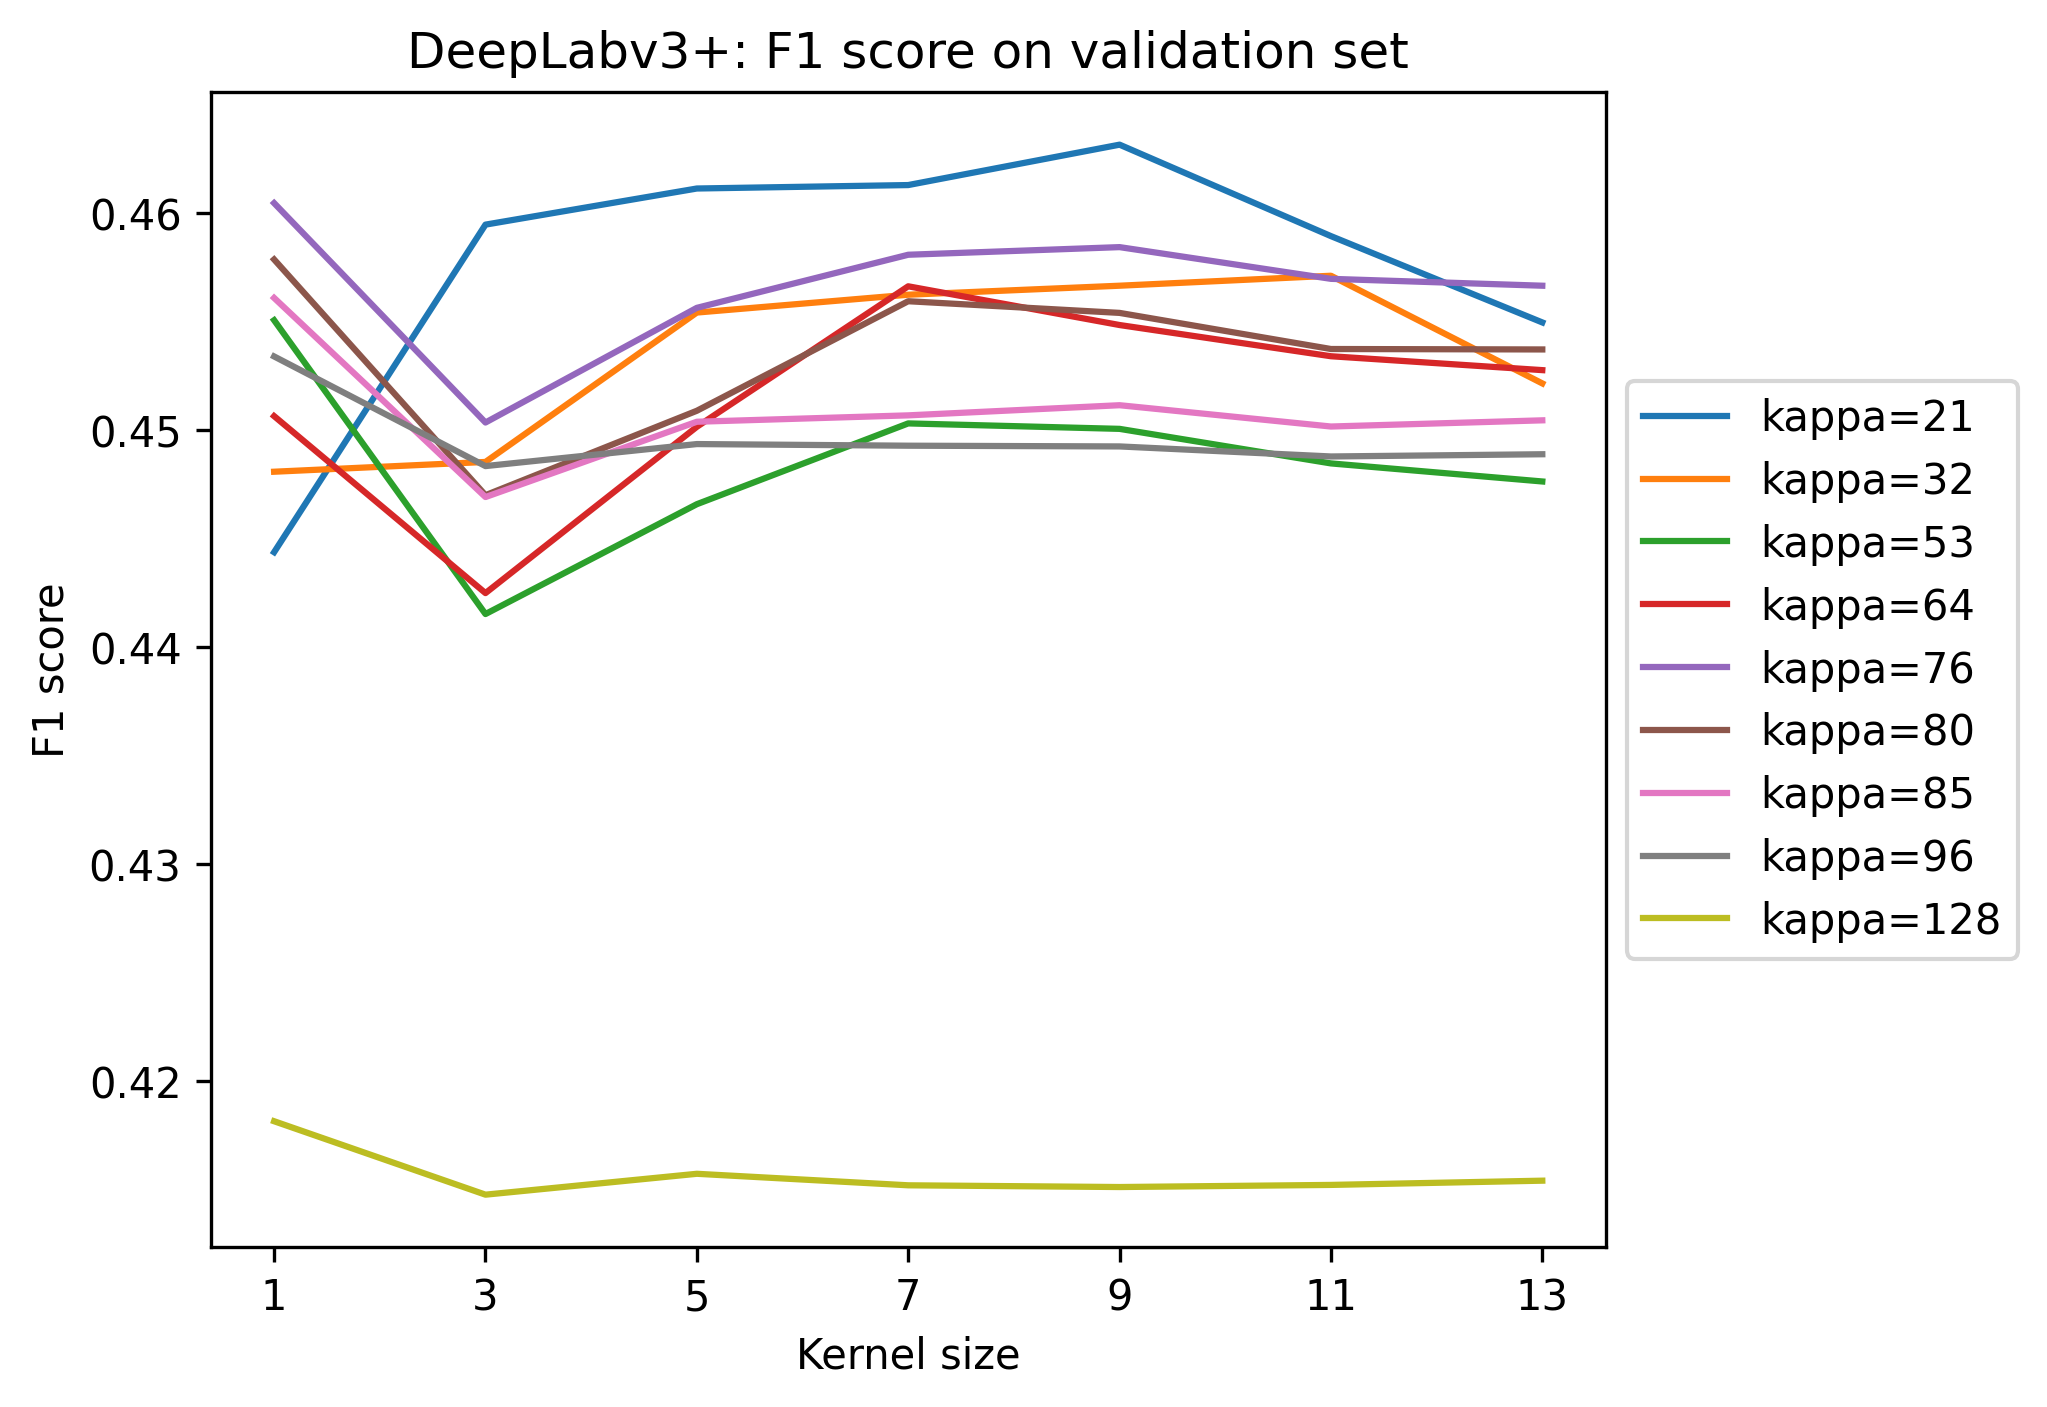
\includegraphics[width=.5\linewidth]{figures/tils/deeplabv3+_f1_kappas_kernels_plot.png}
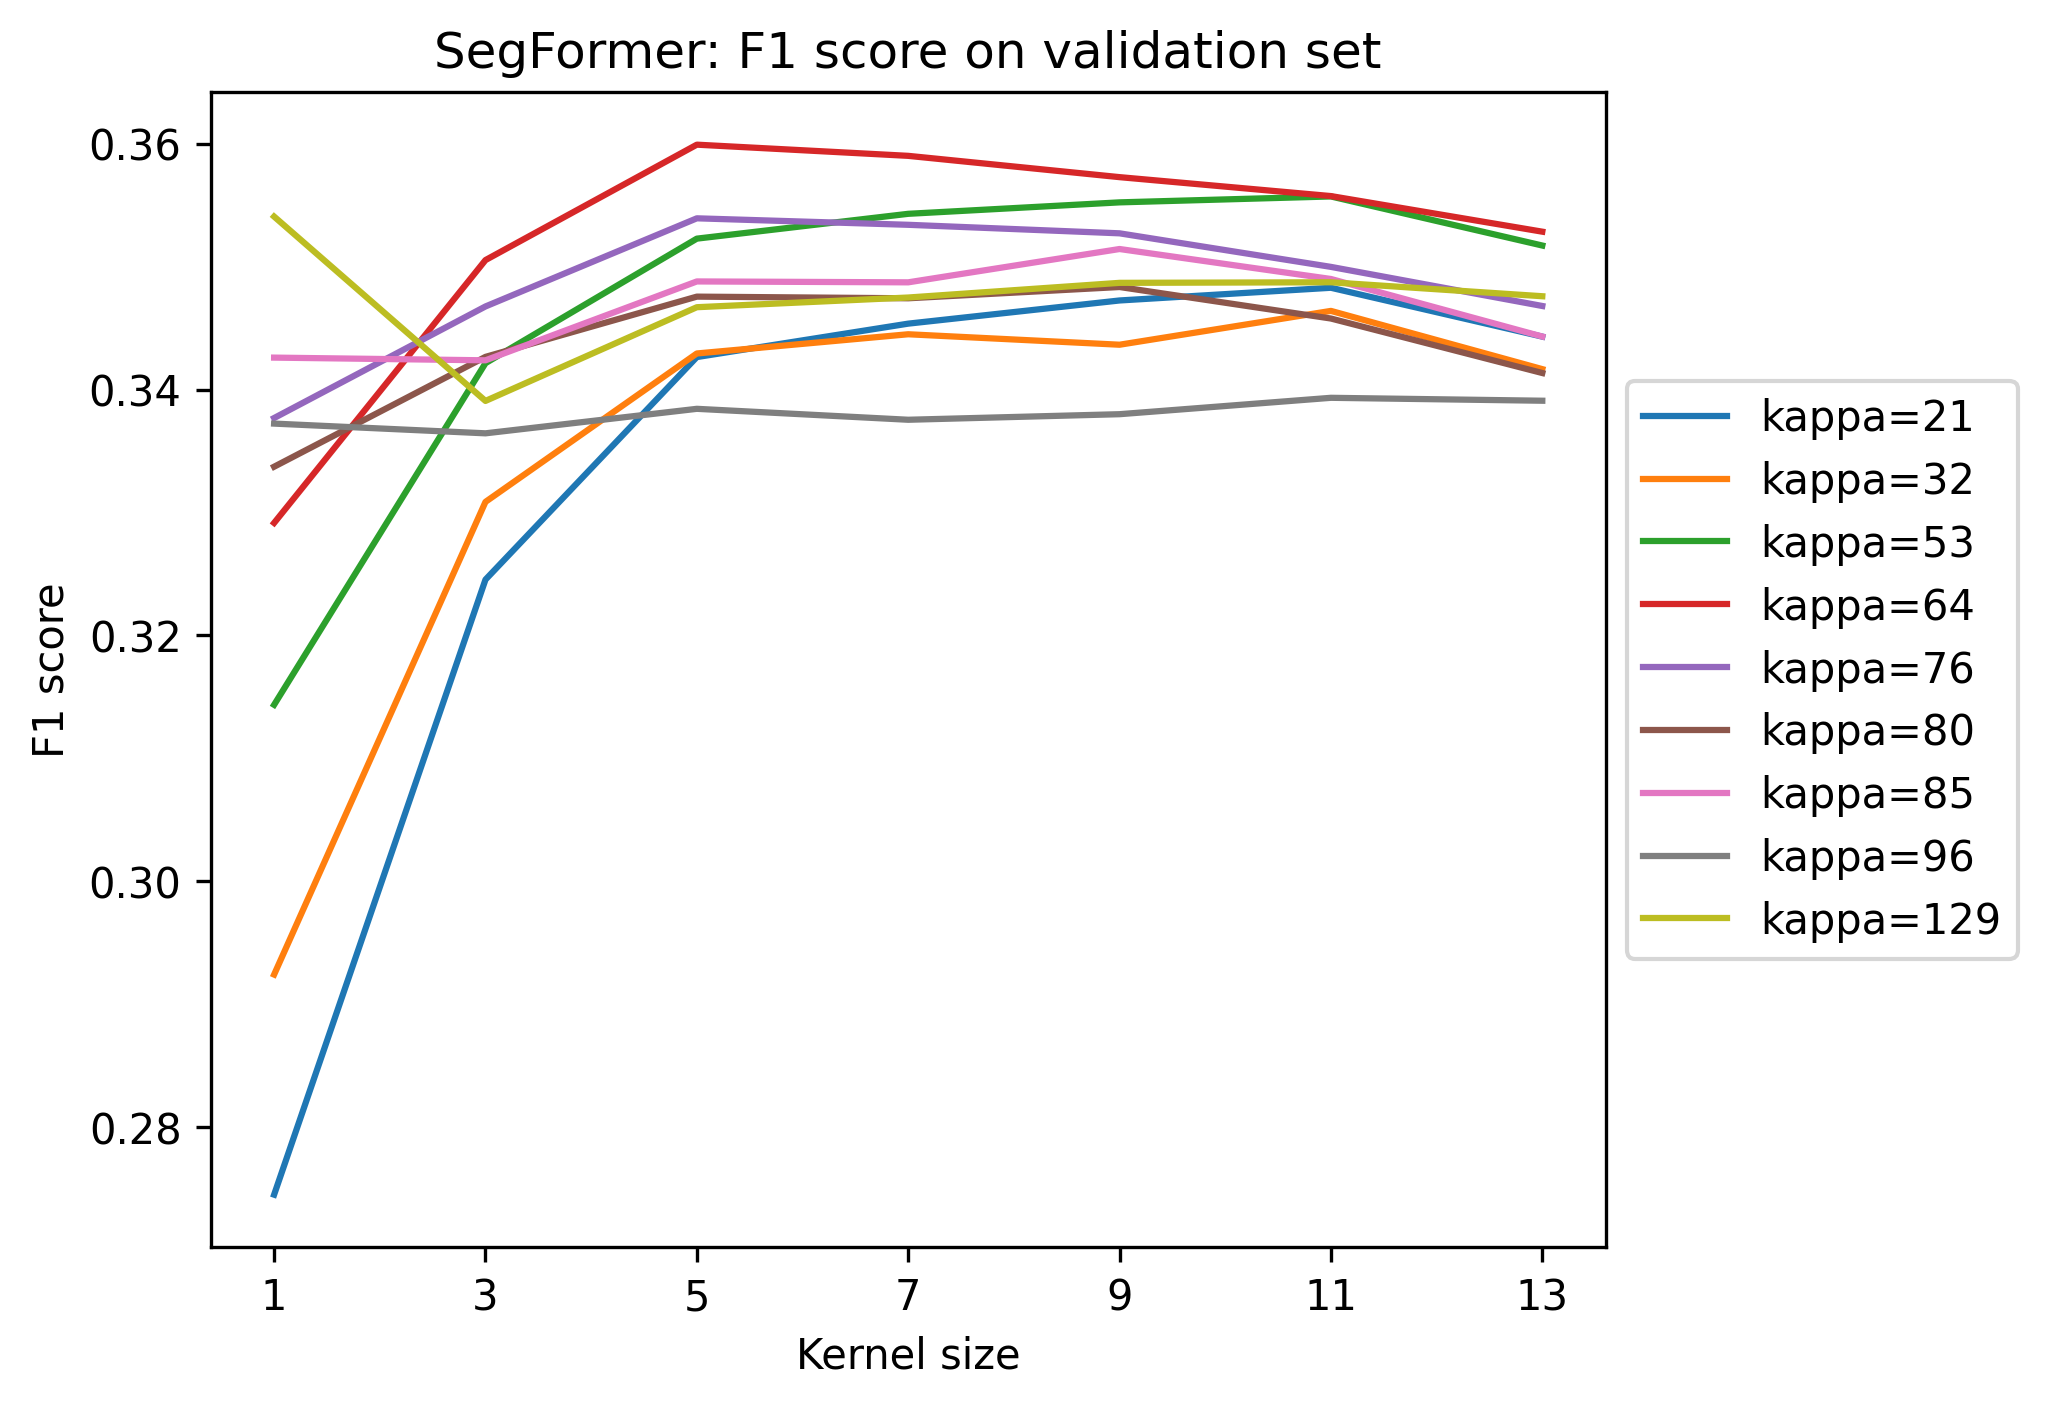
\includegraphics[width=.5\linewidth]{figures/tils/segformer_f1_kappas_kernels_plot.png}
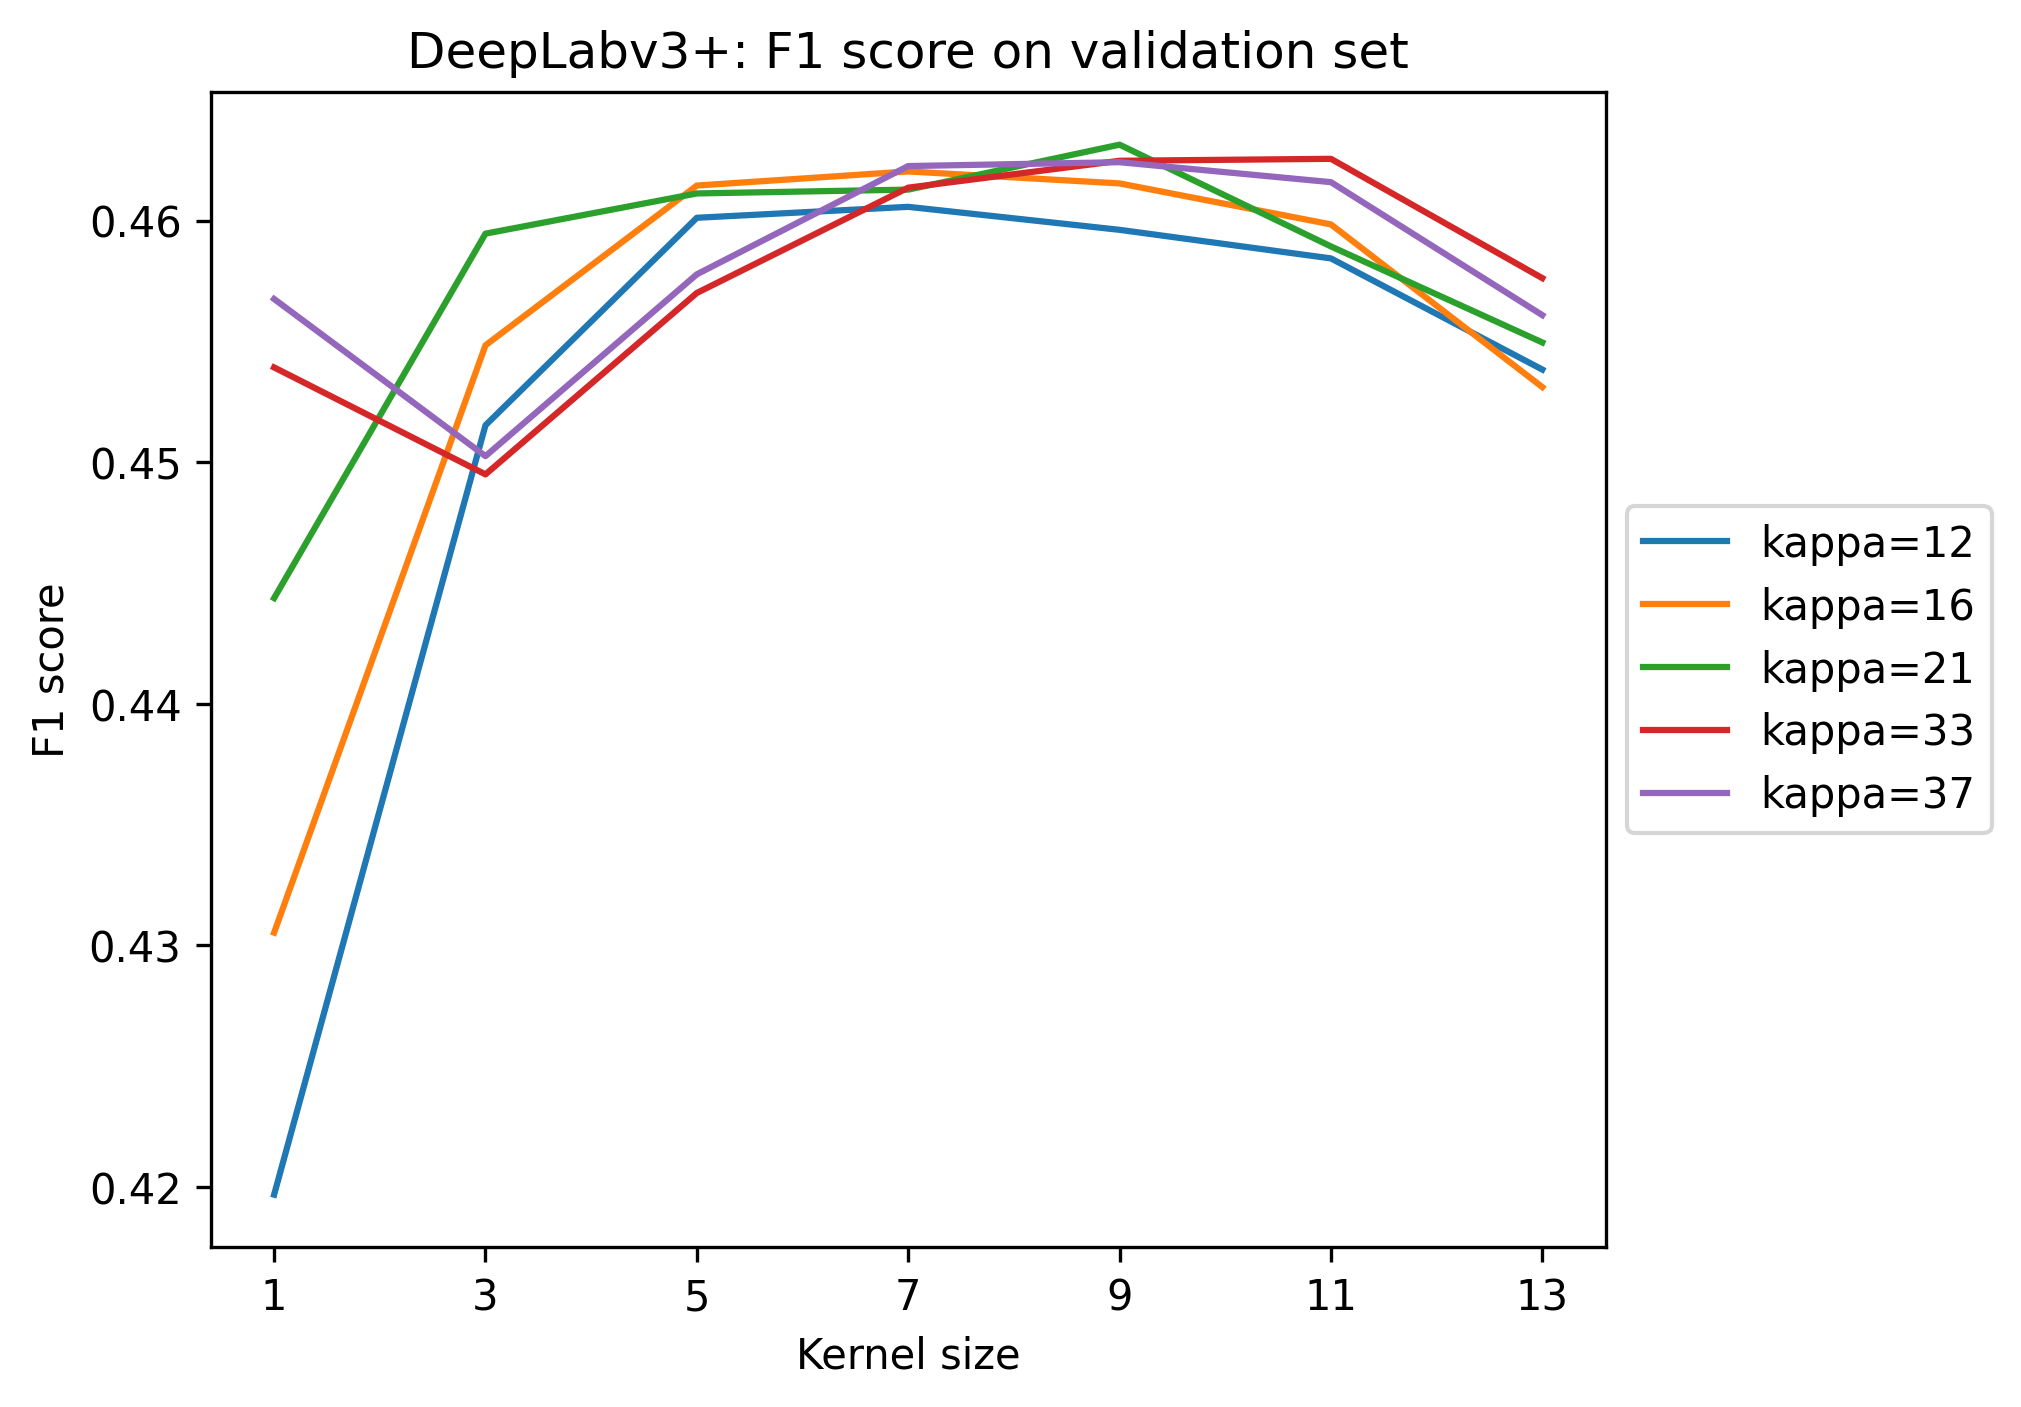
\includegraphics[width=.5\linewidth]{figures/tils/deeplabv3+_f1_kappas_kernels_plot_zooomed.png}
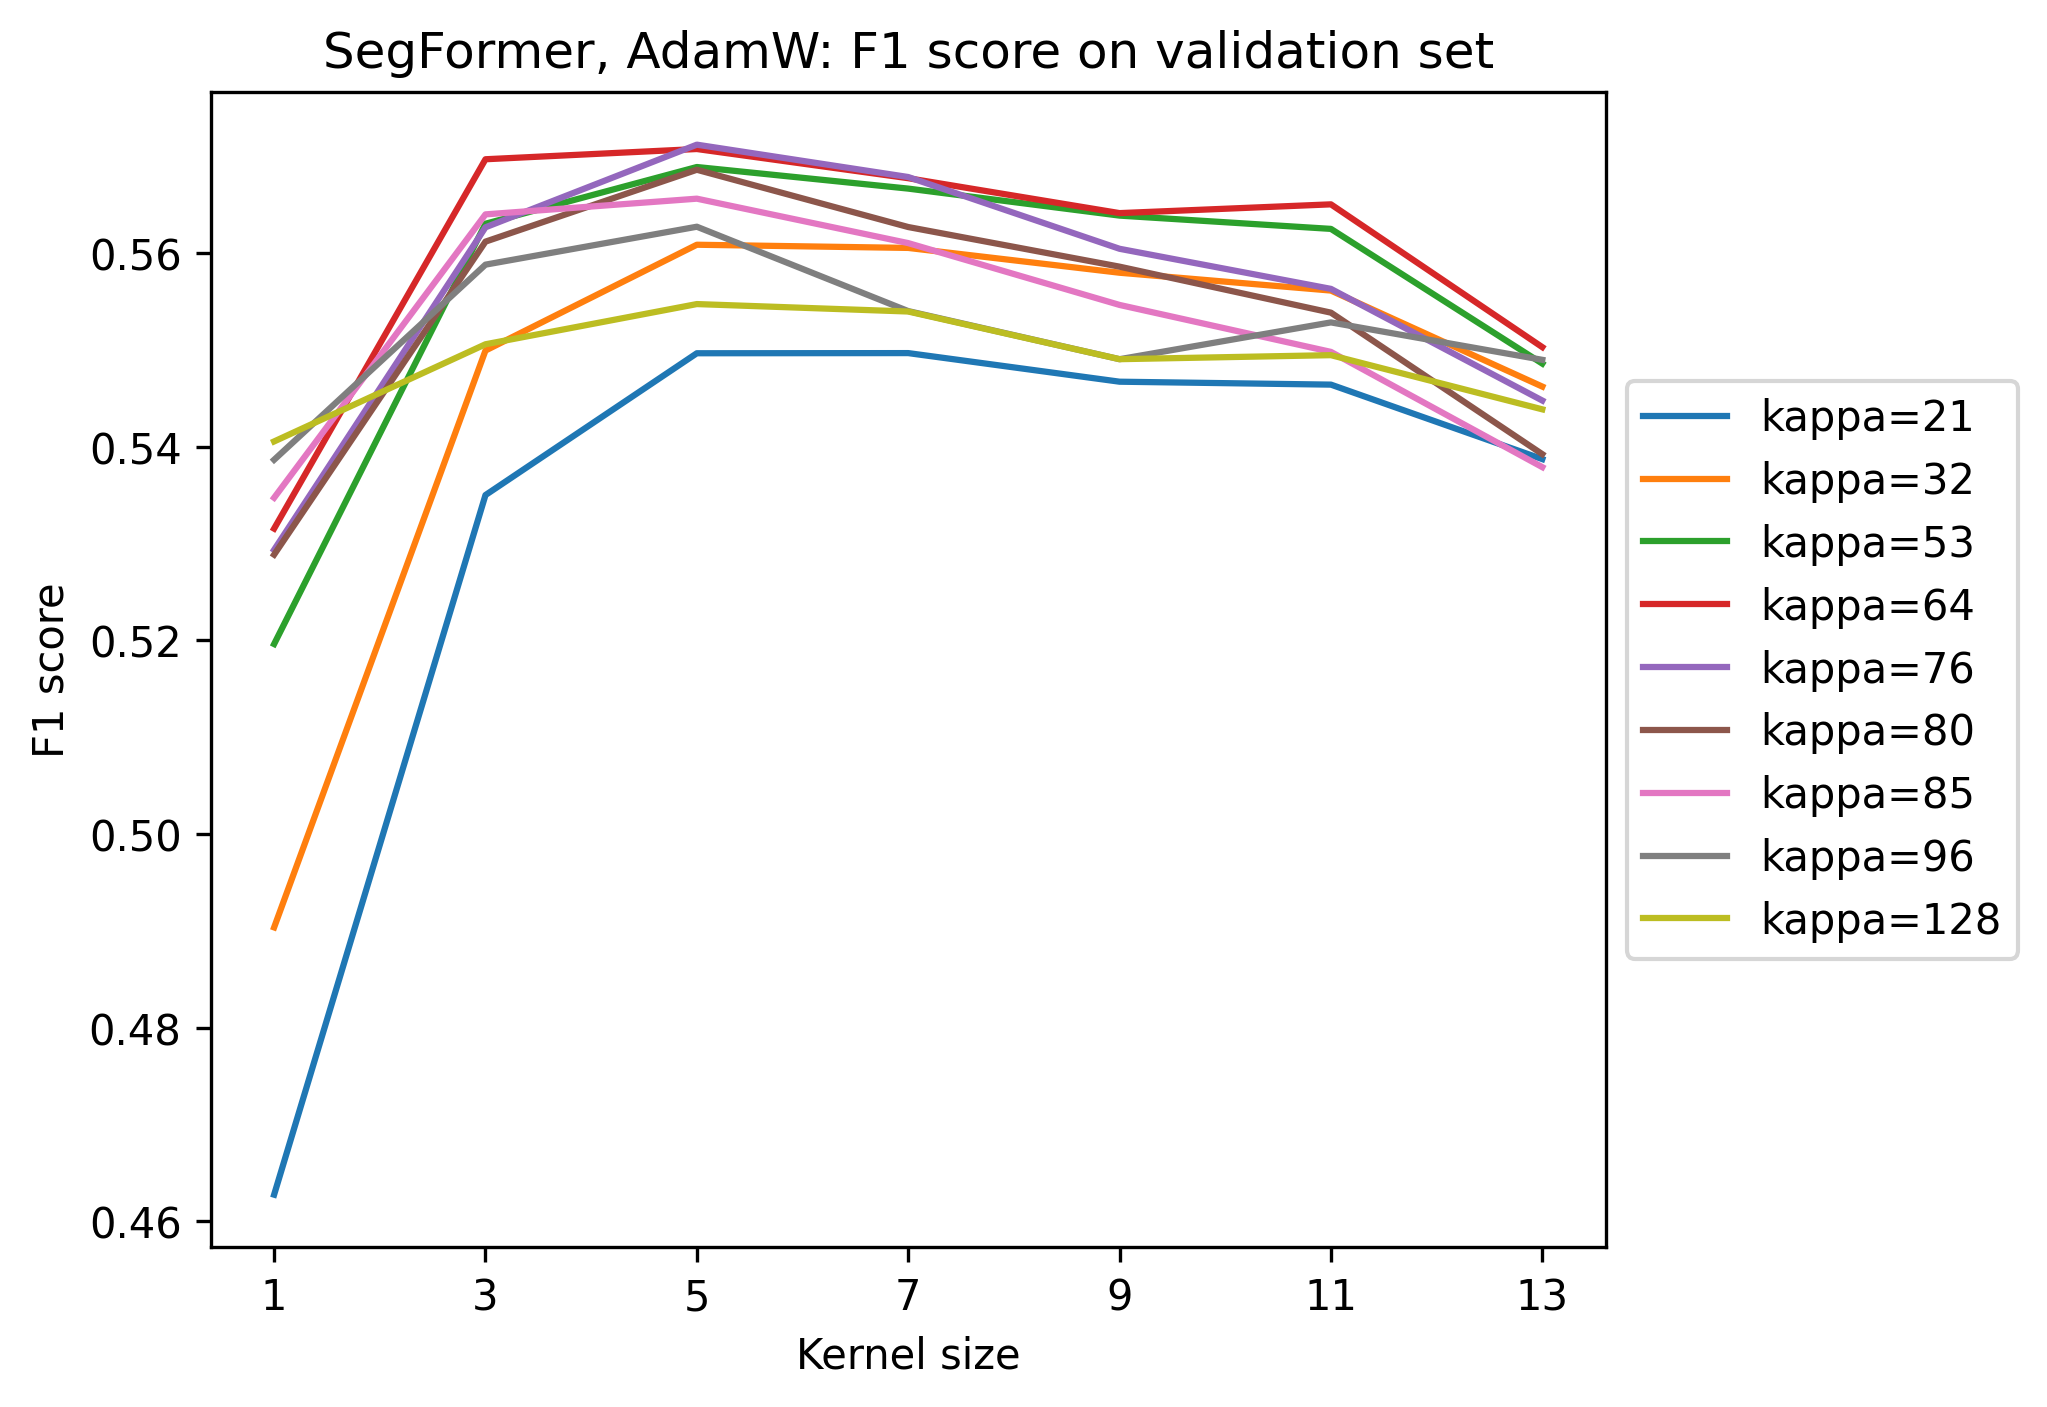
\includegraphics[width=.5\linewidth]{figures/tils/segformer,_adamw_f1_kappas_kernels_plot.png}
\caption{Determination process for best kappa and kernel size for DeepLabv3+
(first in the first row and first in the second row), SegFormer (second in the first row),
and SegFormer with AdamW (second in the second row).}
\label{fig:kappas}
\end{figure}

The final results represented in Table~\ref*{tab:tils_perform} show that SegFormer
model with AdamW optimizer strongly outperforms DeepLabv3+ and simple SegFormer.
Furthermore, while distinguishing the F1 scores between ROIs originating from different medical
centers in Figure~\ref*{fig:tils_dice_boxplots}, SegFormer AdamW results show
significantly better results in all subgroups.
\begin{figure}[H]
    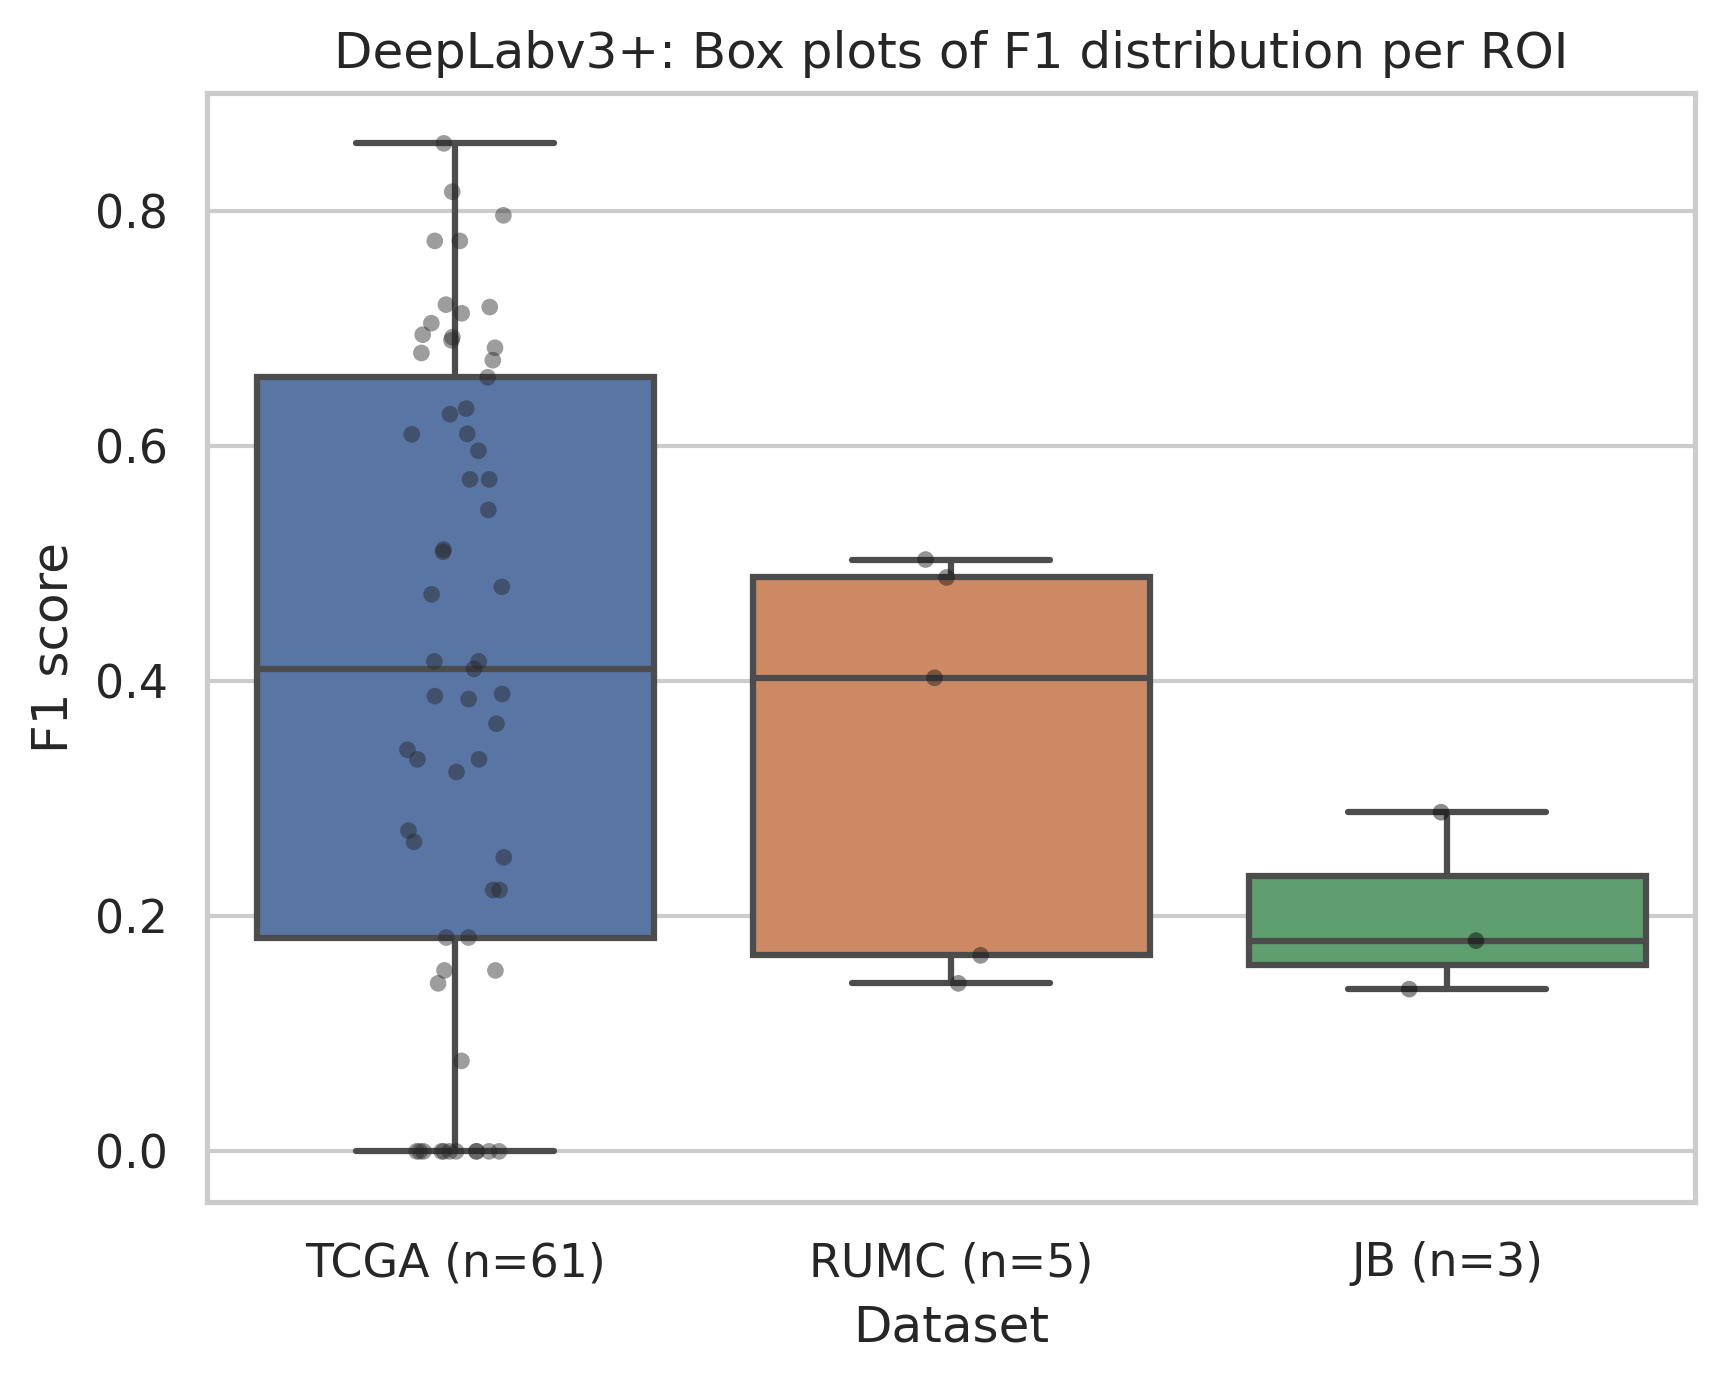
\includegraphics[width=.32\linewidth]{figures/tils/deeplabv3+_F1_roi_adj.png}
    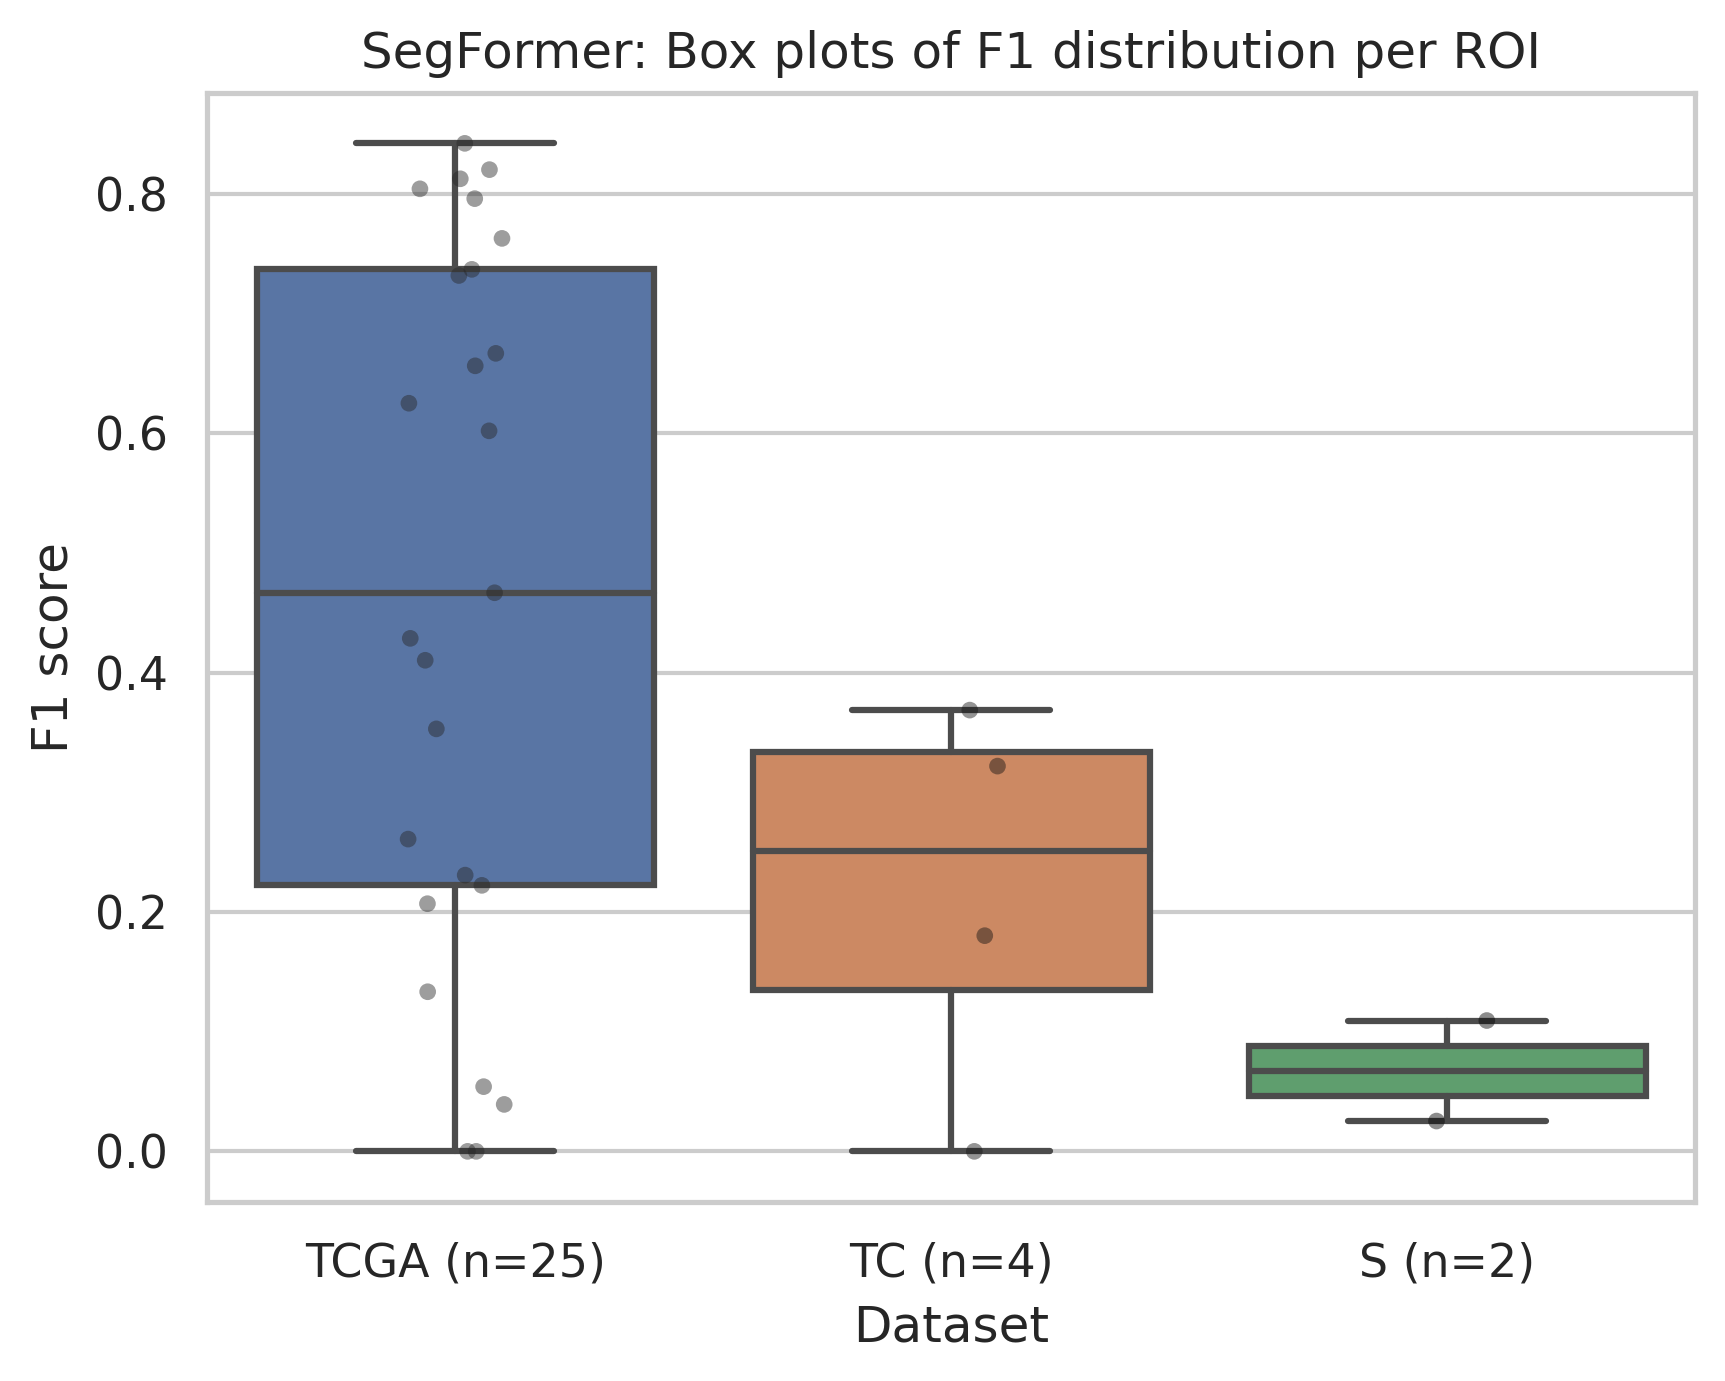
\includegraphics[width=.32\linewidth]{figures/tils/segformer_F1_roi_adj.png}
    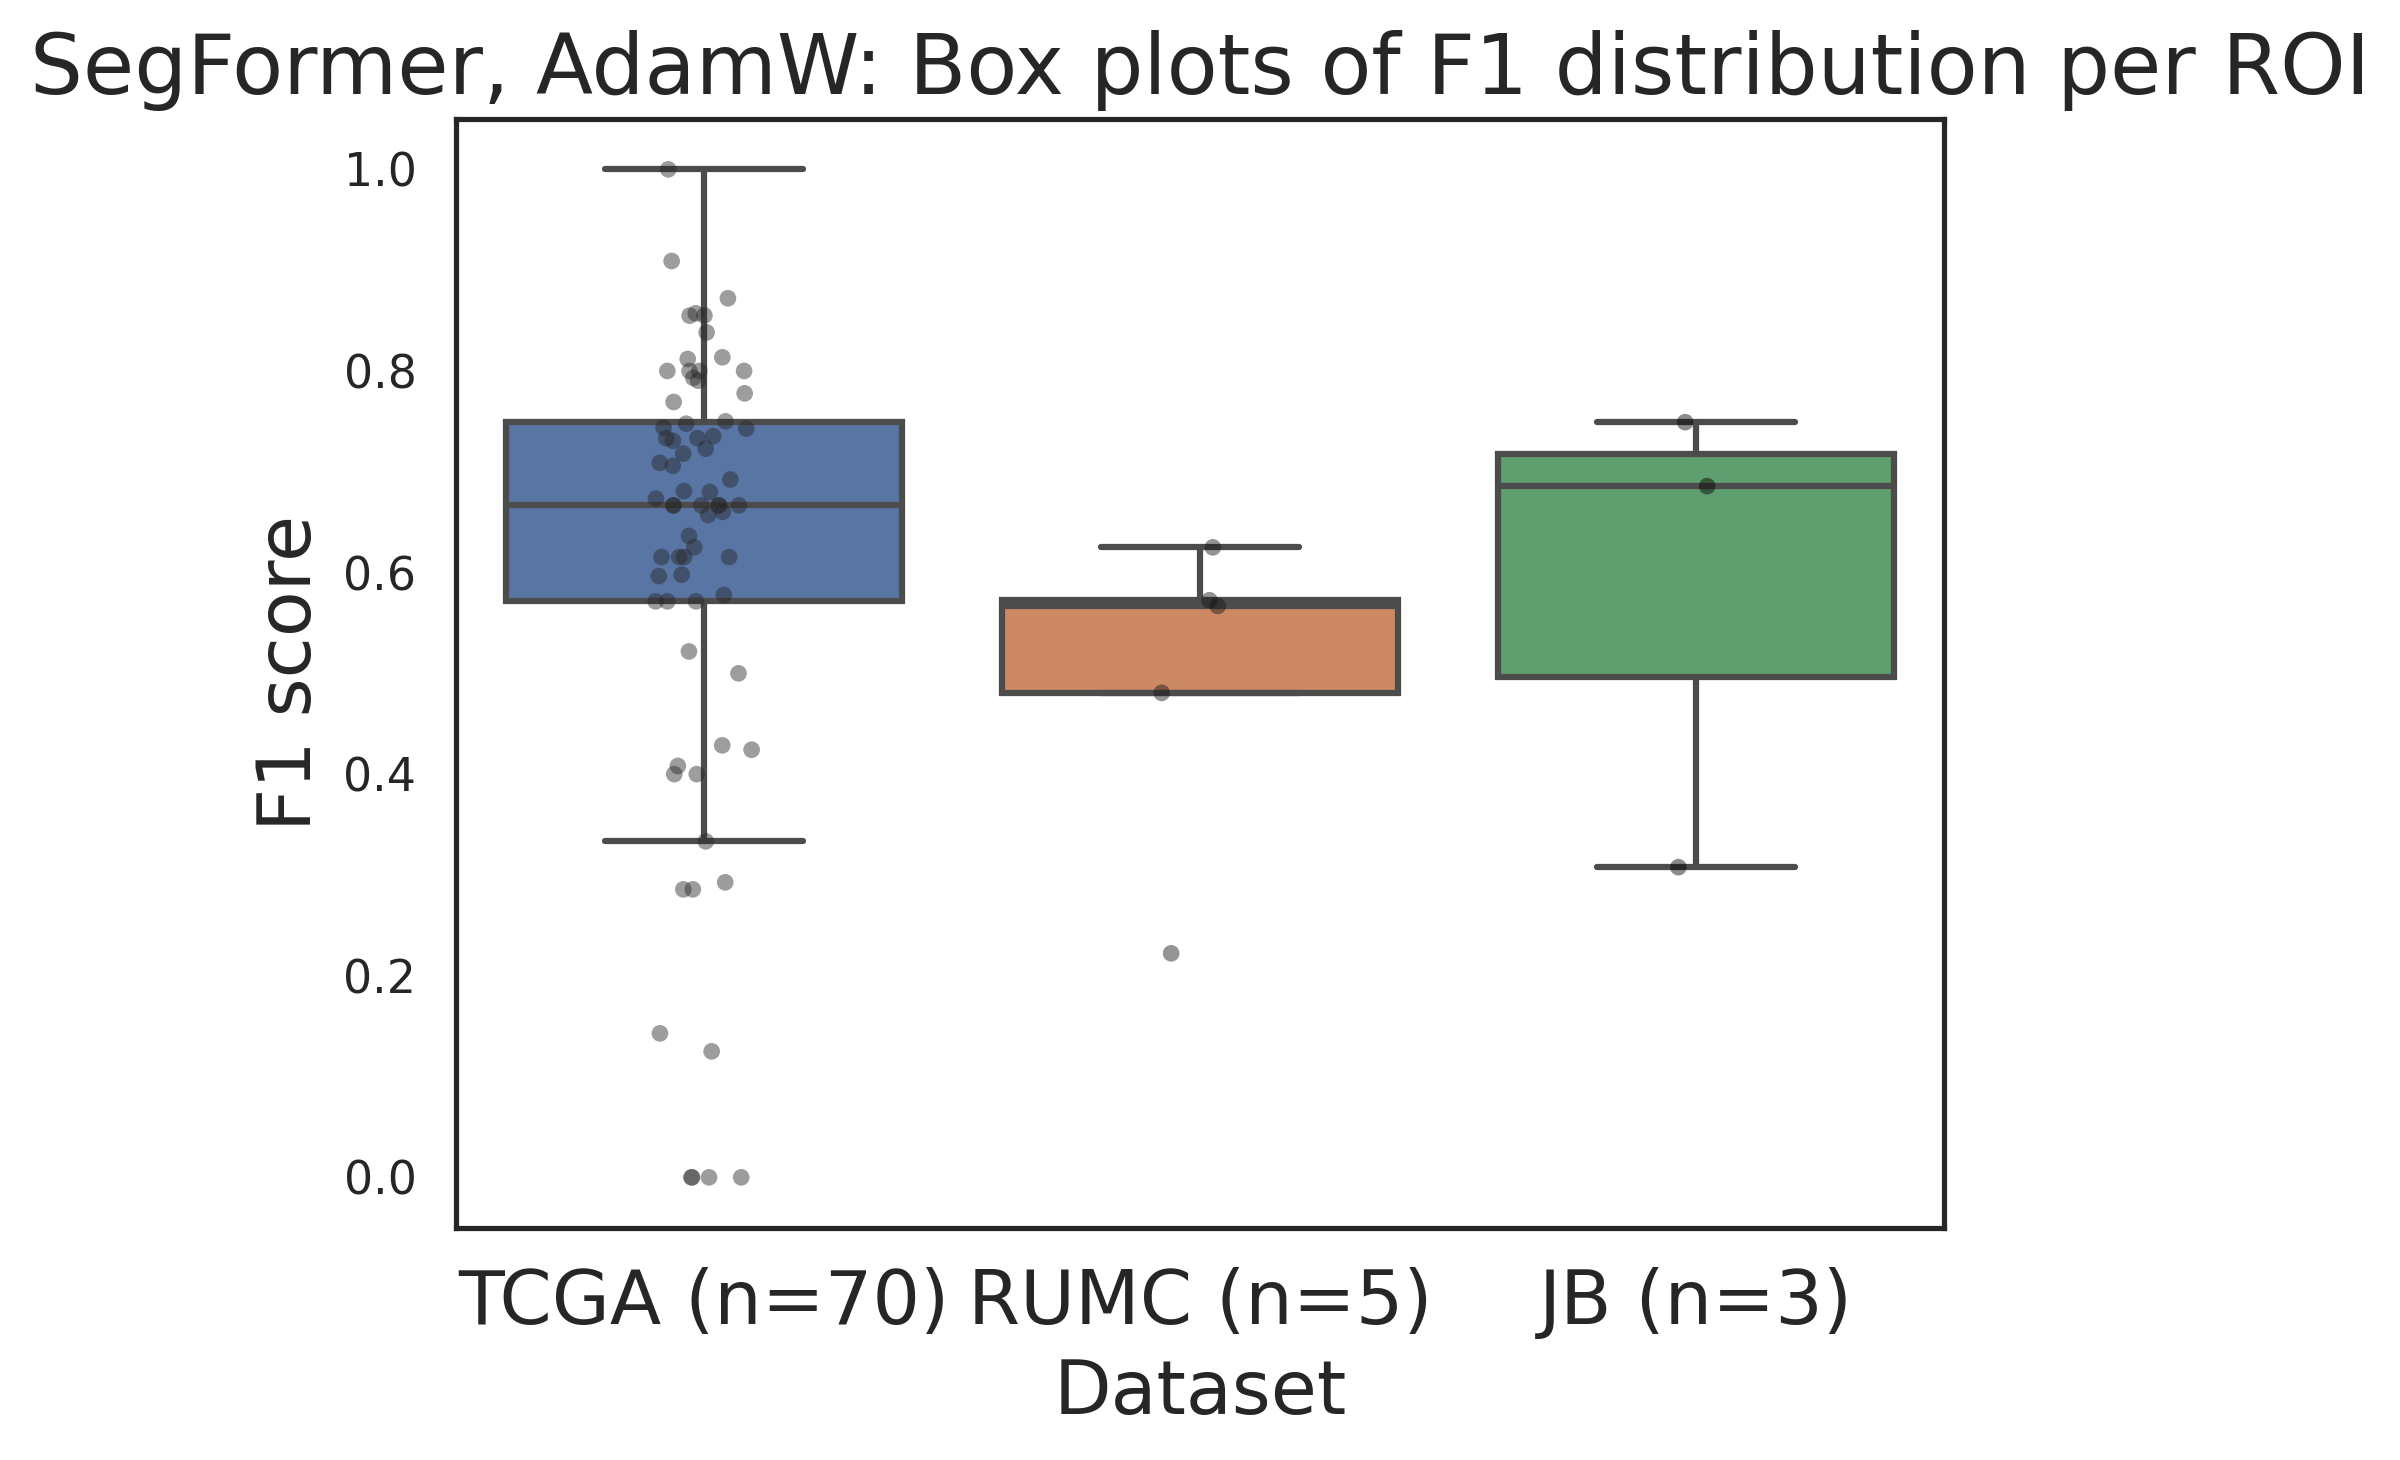
\includegraphics[width=.32\linewidth]{figures/tils/segformer,_adamw_F1_roi_adj.png}
    \caption{Boxplots of dice score across three datastes (TCGA-BRCA, RUMC, JB) with
    maximum allowed distance between ground truth and prediction equals 10 pixels (5 \textmu m).}
    \label{fig:tils_dice_boxplots}
\end{figure}
Interestingly the precision boxplots
in Figure~\ref*{fig:tils_pr_r_boxplots} do not show such an unequivocal superiority,
where in the JB subgroup simple SegFormer manages to predict fewer false positives and 
(n=2) indicates that the model managed to predict empty ROI as a complete rest region,
which is not the case for any other model.
In more detailed
Figure~\ref*{fig:TCGA-D8-A142_tils} one can see the intermediate steps of
how the posteriors are simplified into point segmentations and later the misted,
falsely annotated and correct TILs can be compared. Even on the level of posteriors
(overlayed with H\&E image), it is visible that SegFormer AdamW manages to detect
more regions, especially closer to the border of the image. The grids in Figure~\ref*{fig:TCGA-D8-A142_tils}
were added for readers' convenience and are not artifacts. Taking into account all
discussions above and the overall better performance, the SegFromer AdamW was
considered the best model, and the model with the highest pixel-wise dice score
on the validation set was taken to the next step. 

\begin{figure}[H]
    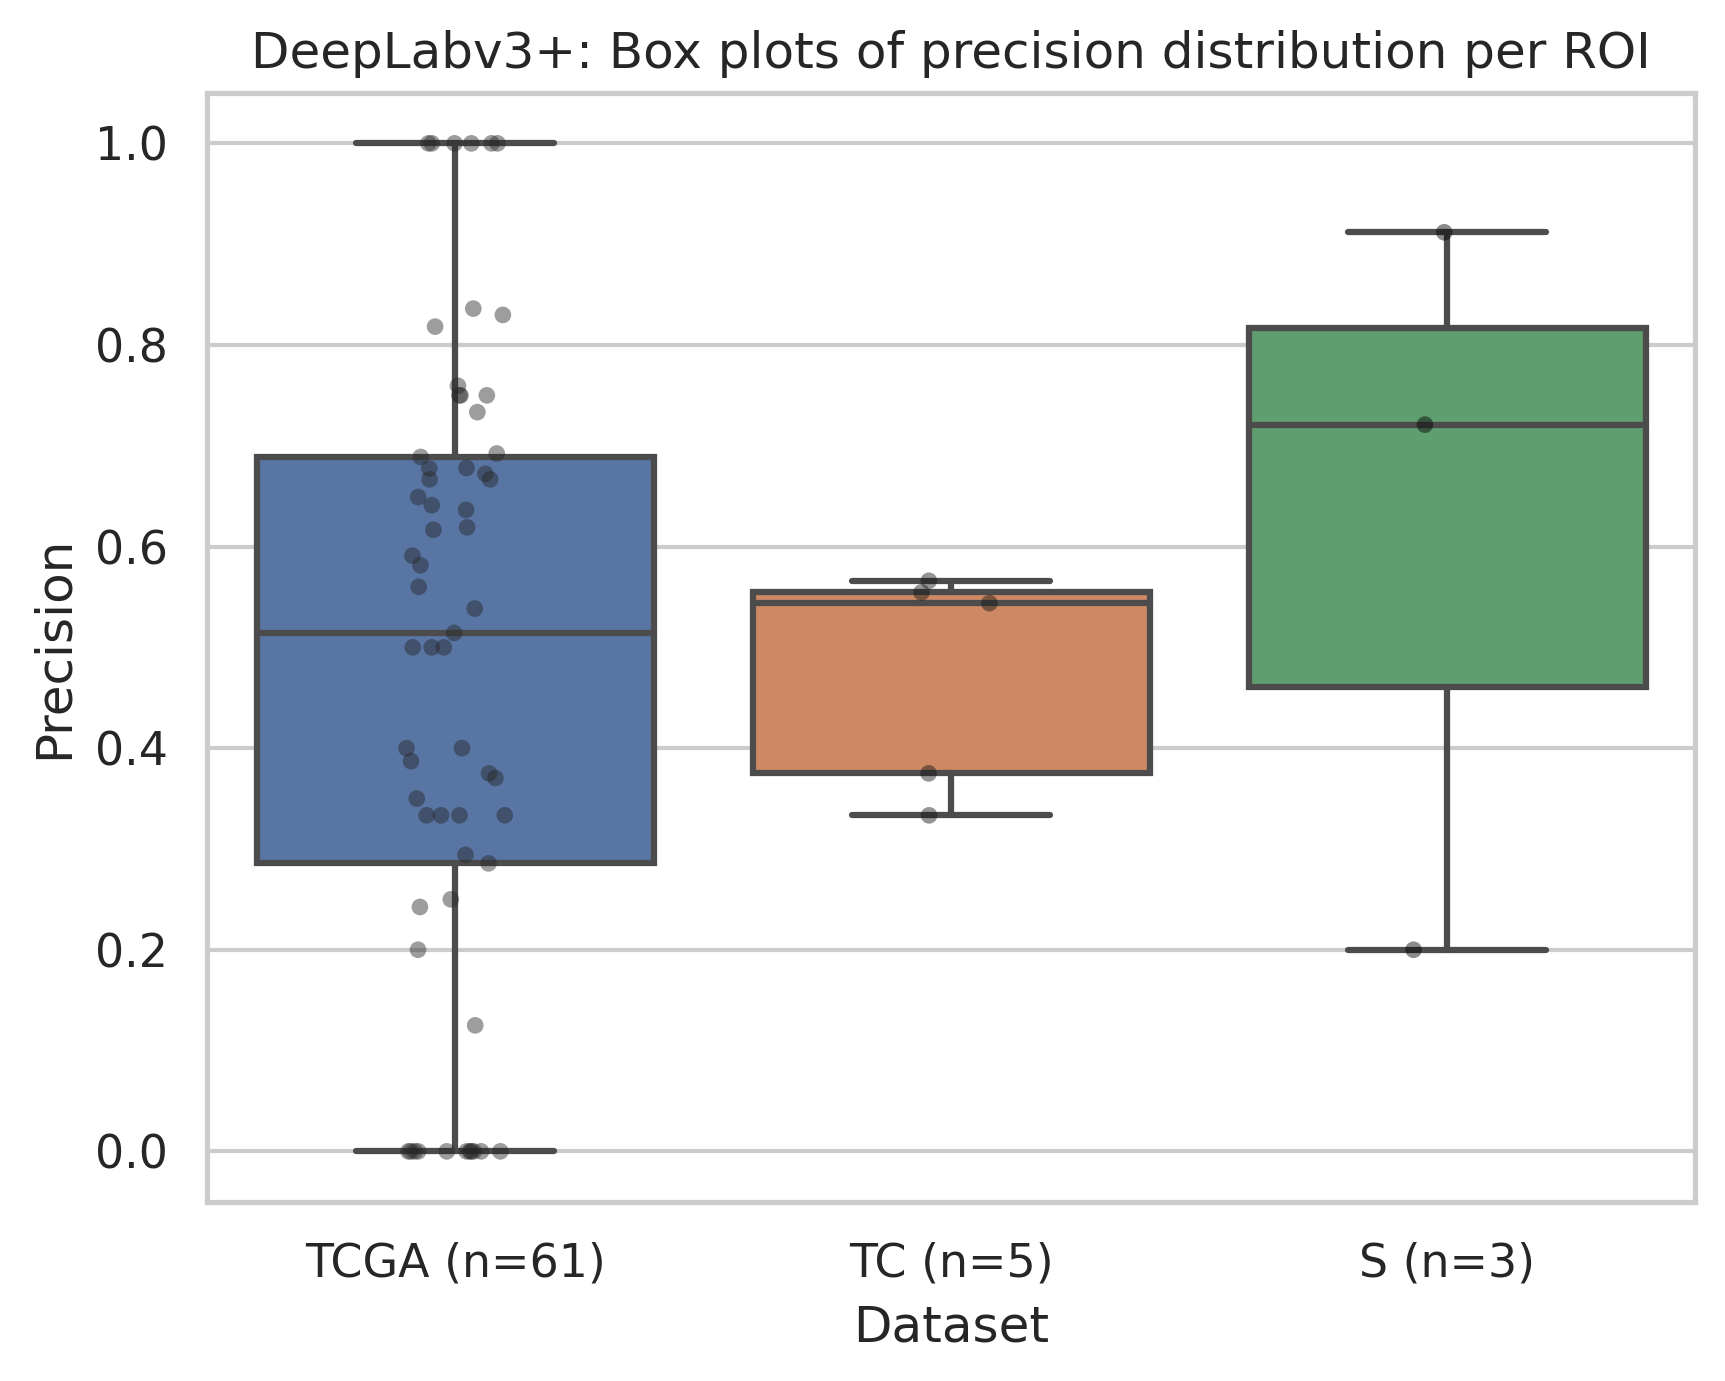
\includegraphics[width=.32\linewidth]{figures/tils/deeplabv3+_precision_roi_adj.png}
    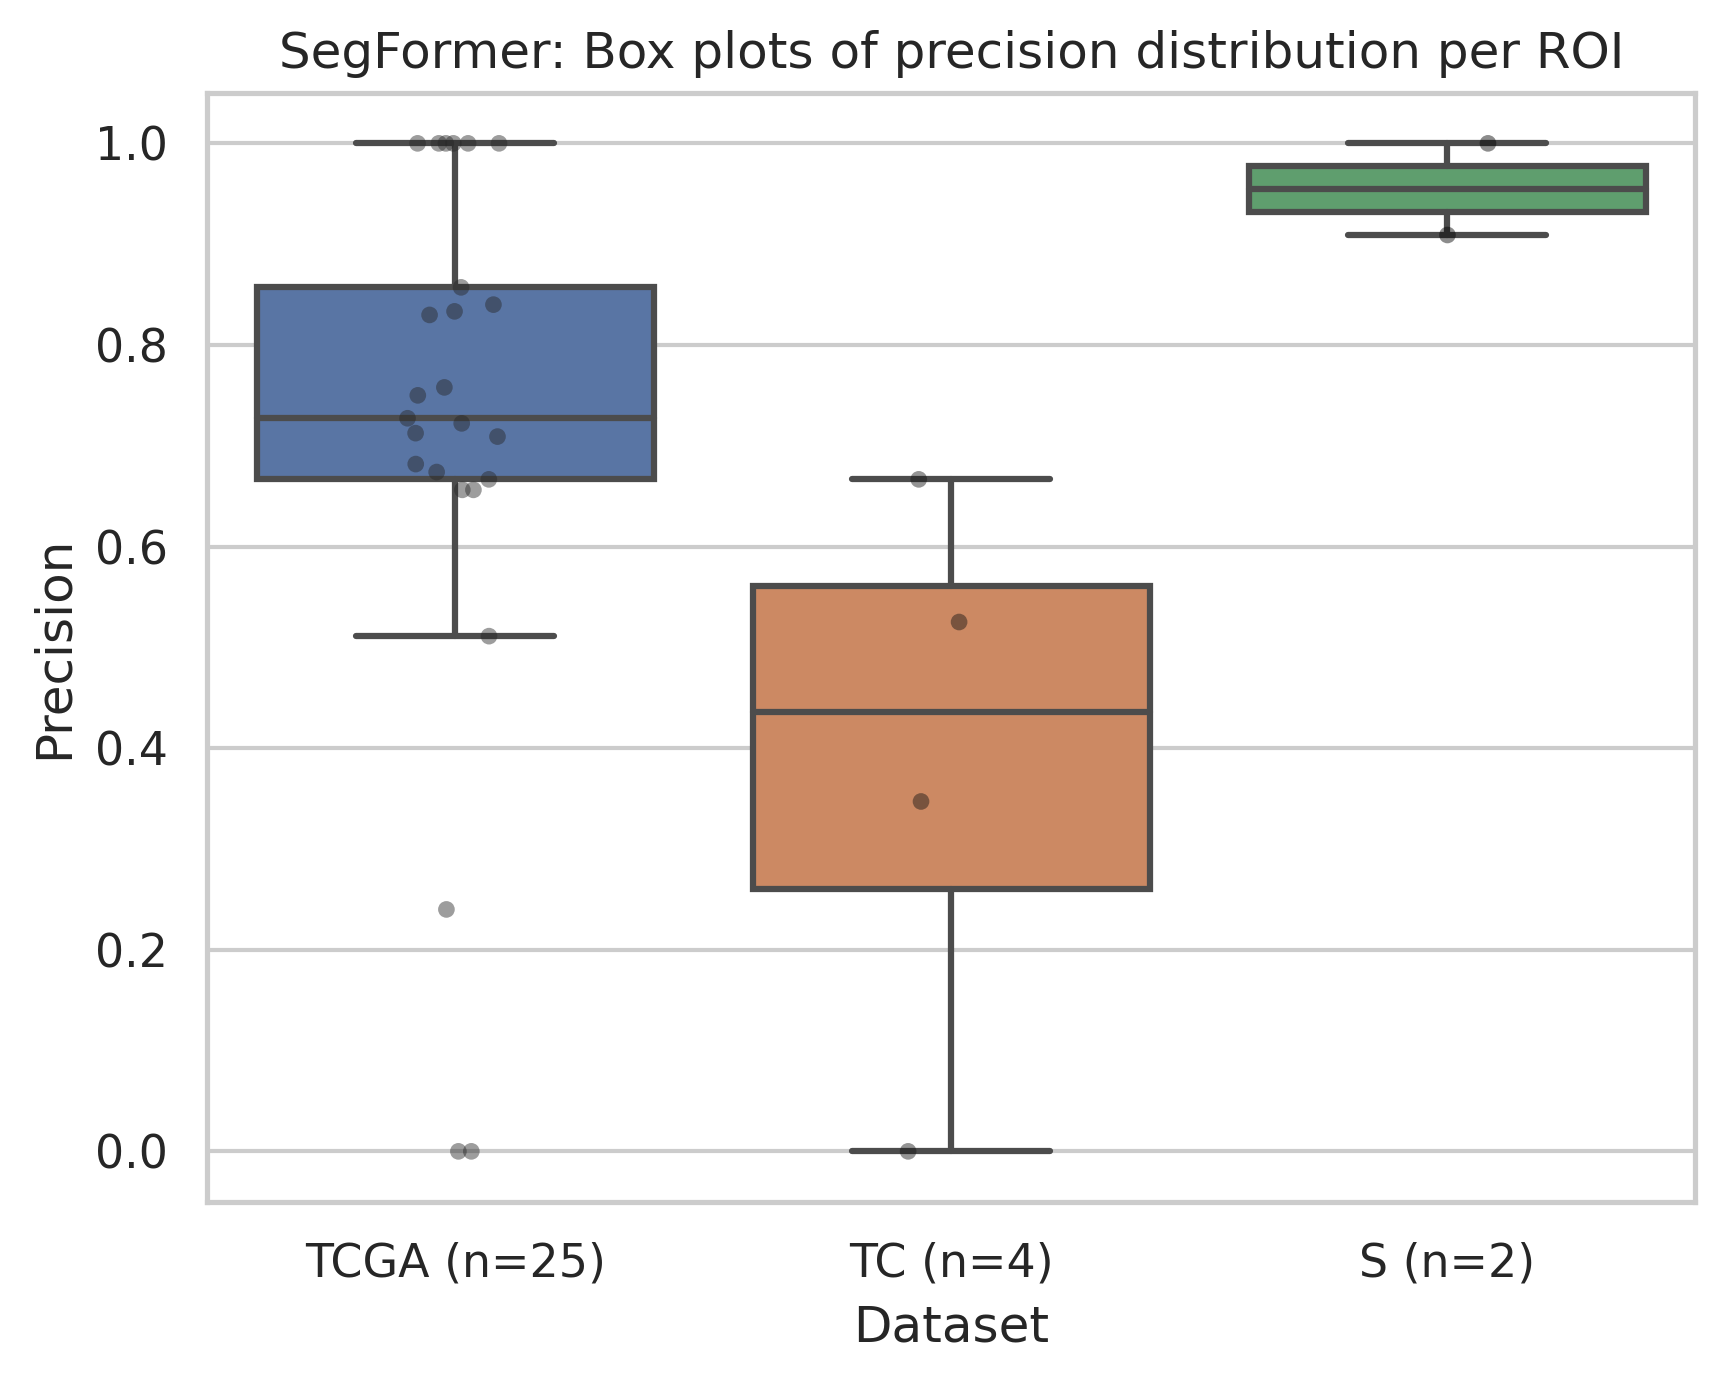
\includegraphics[width=.32\linewidth]{figures/tils/segformer_precision_roi_adj.png}
    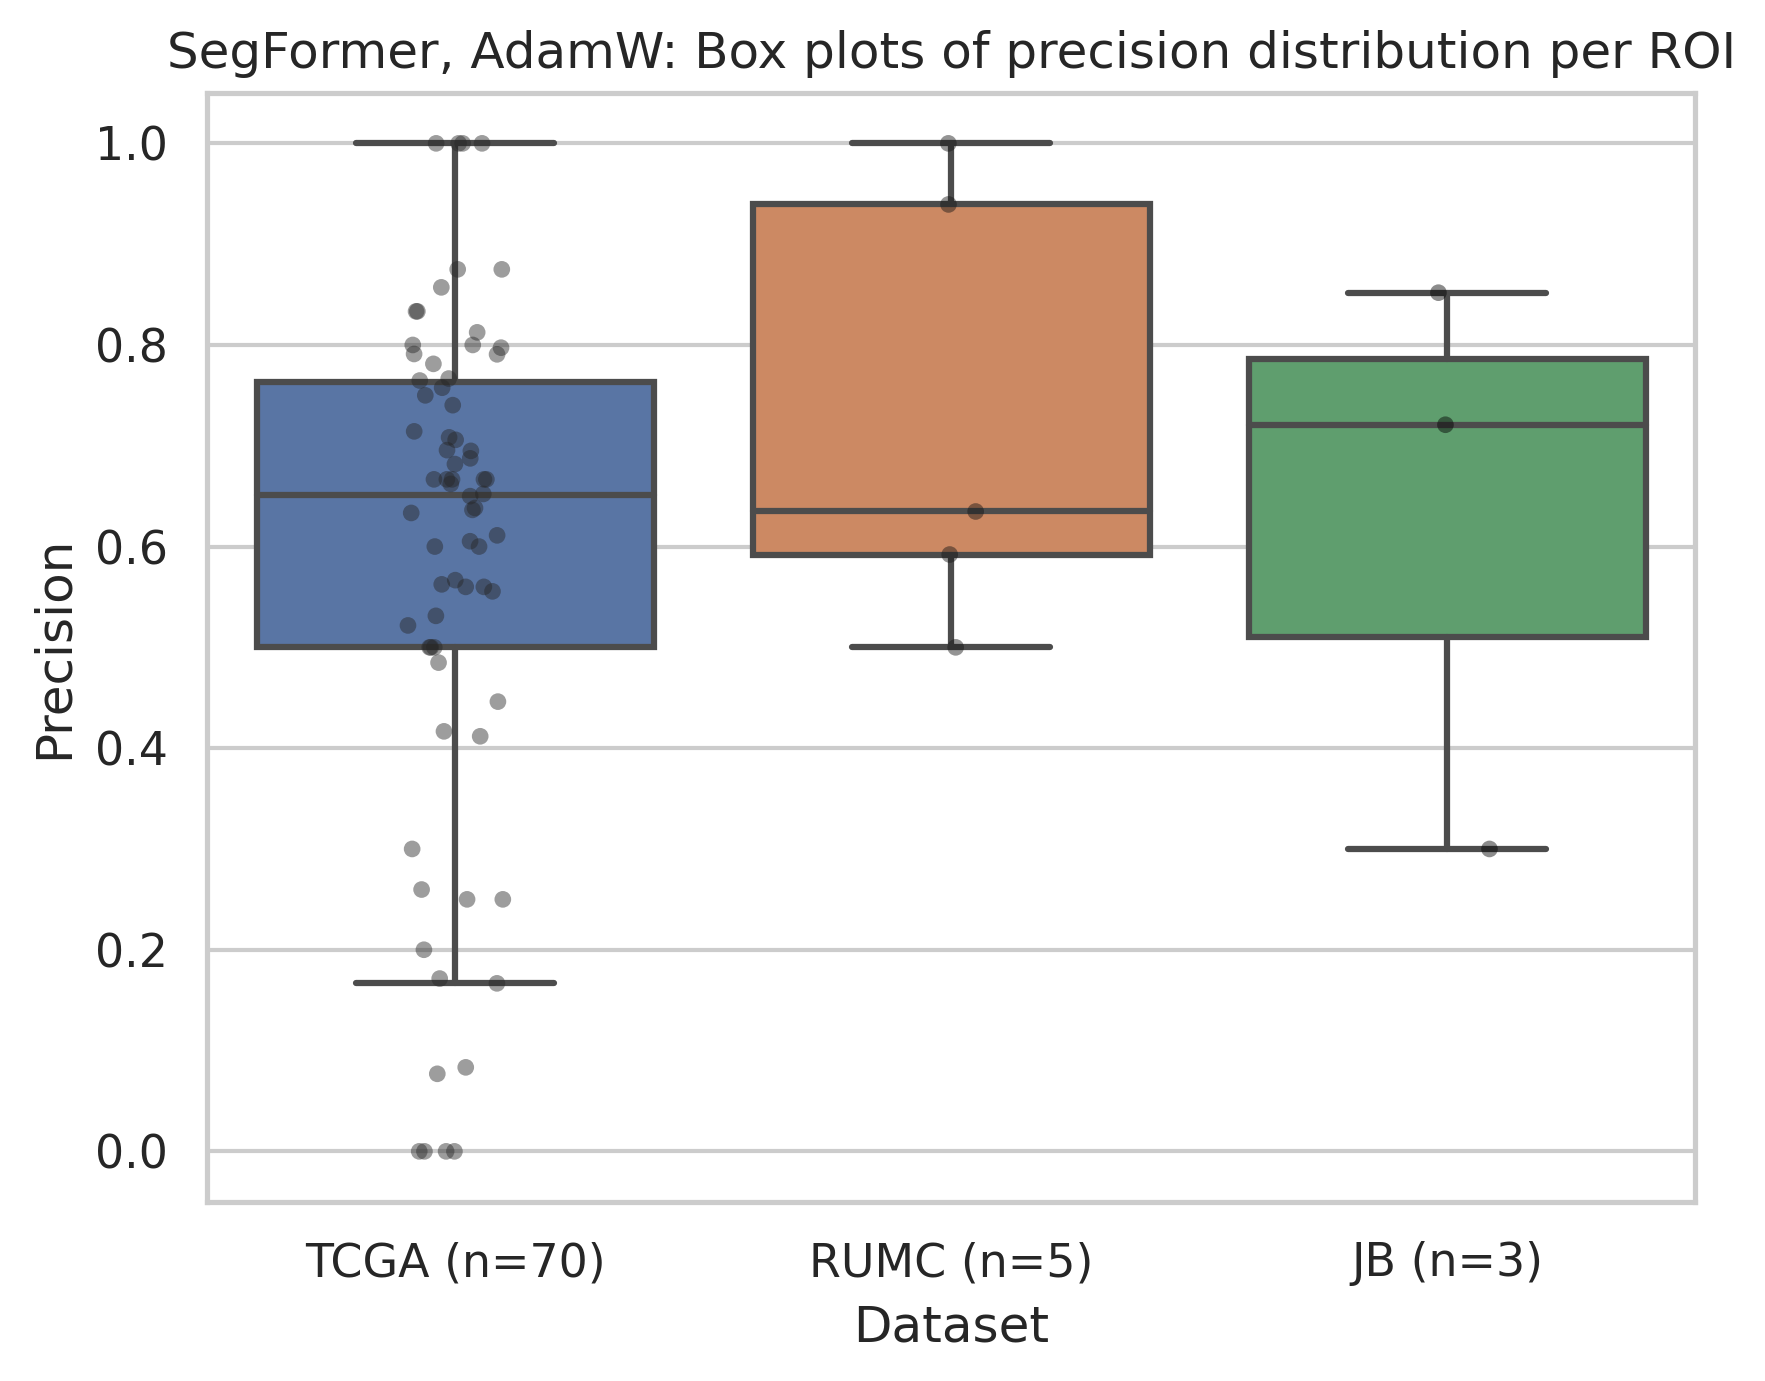
\includegraphics[width=.32\linewidth]{figures/tils/segformer,_adamw_precision_roi_adj.png}
    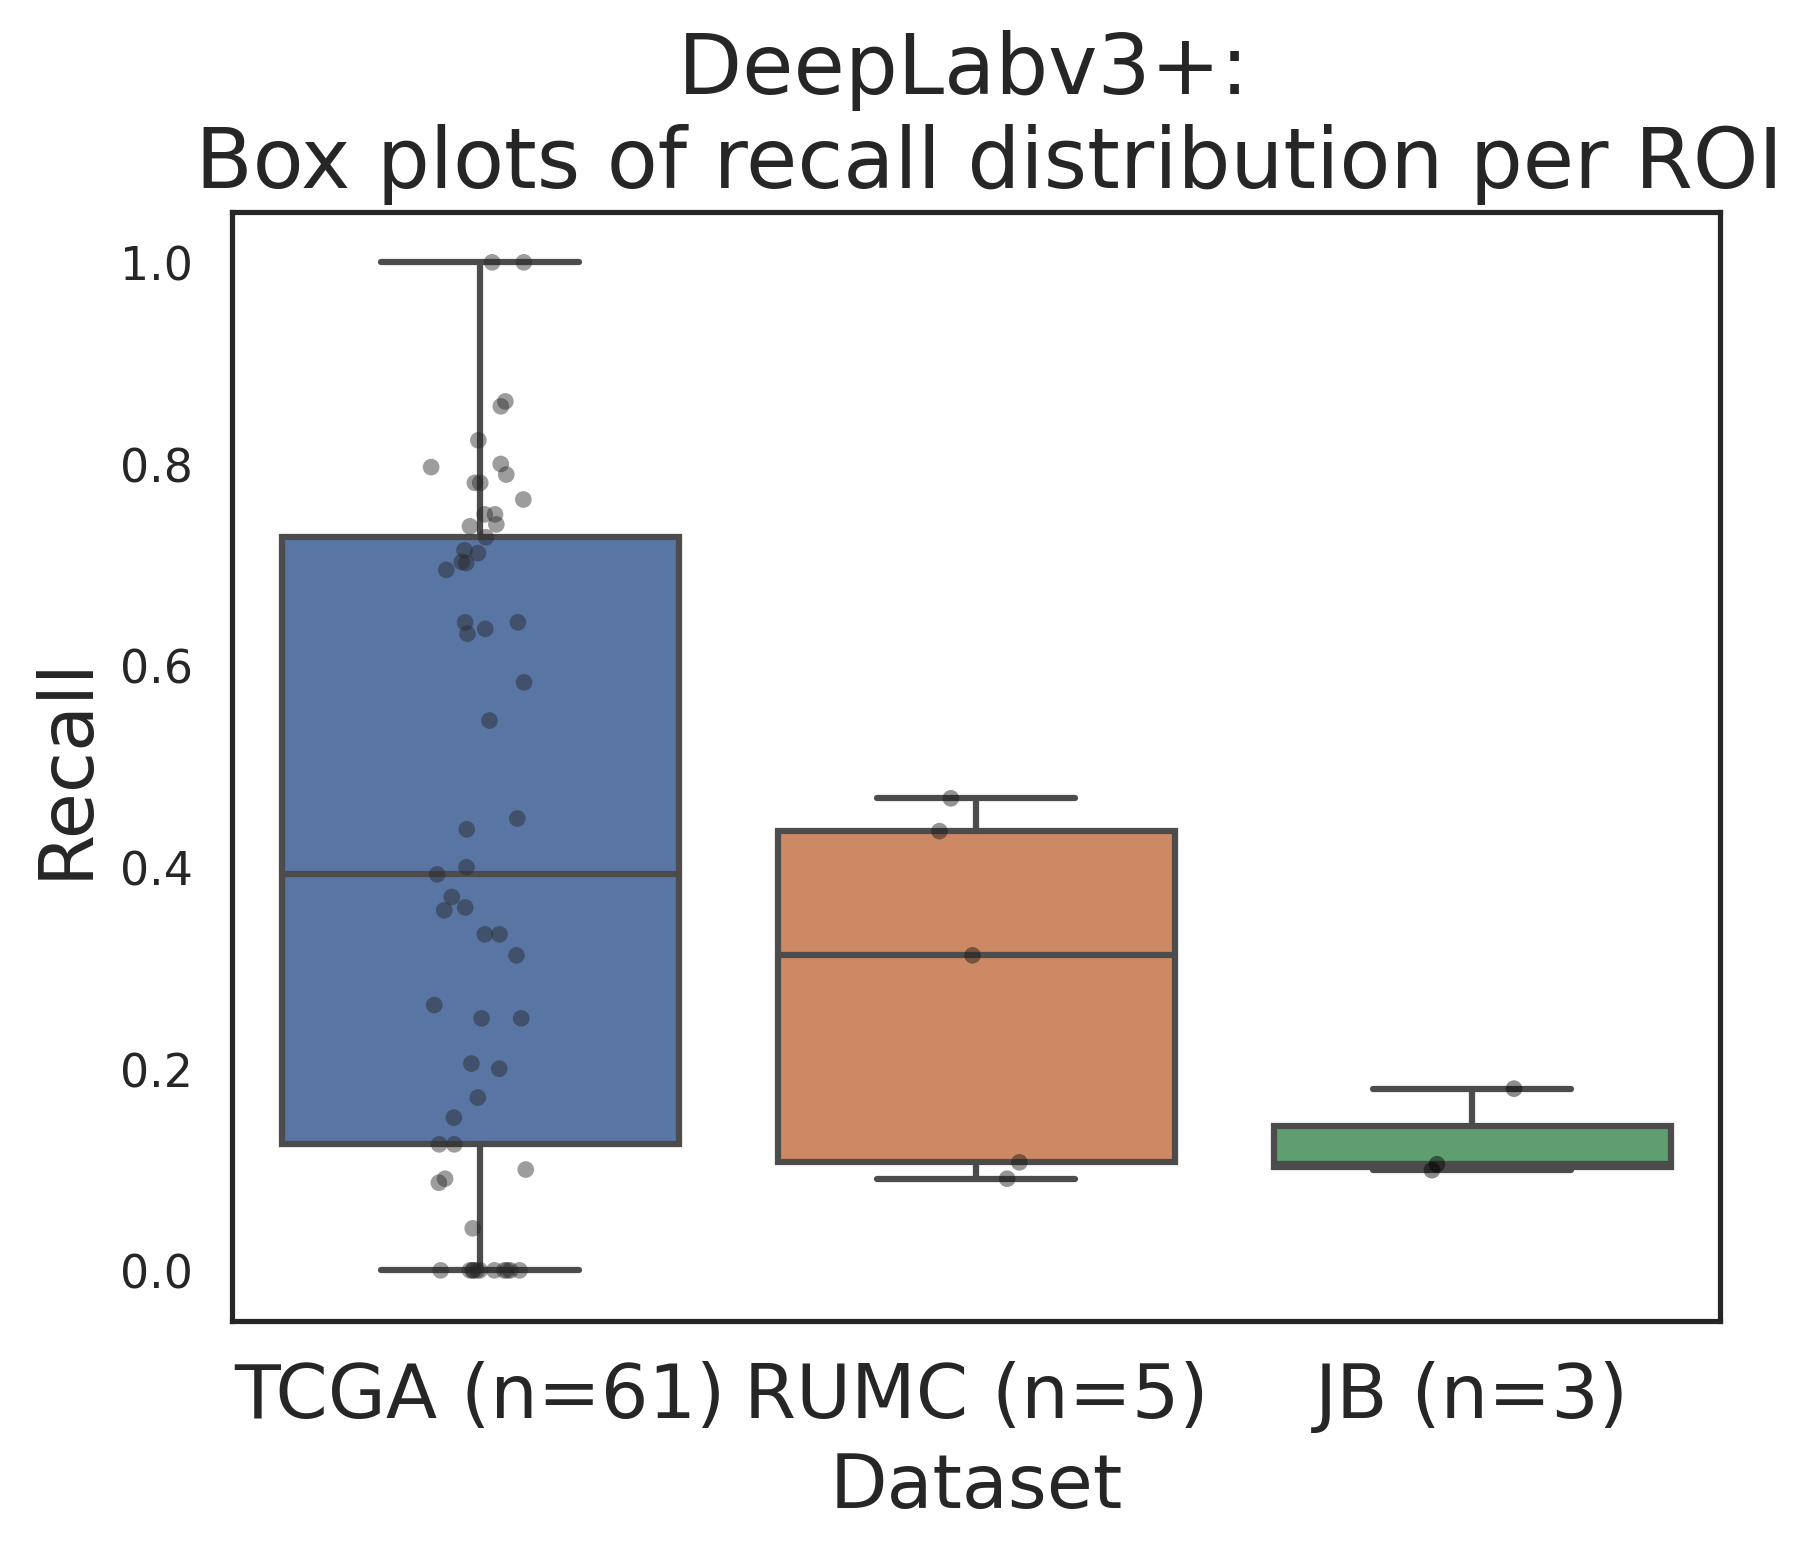
\includegraphics[width=.32\linewidth]{figures/tils/deeplabv3+_recall_roi_adj.png}
    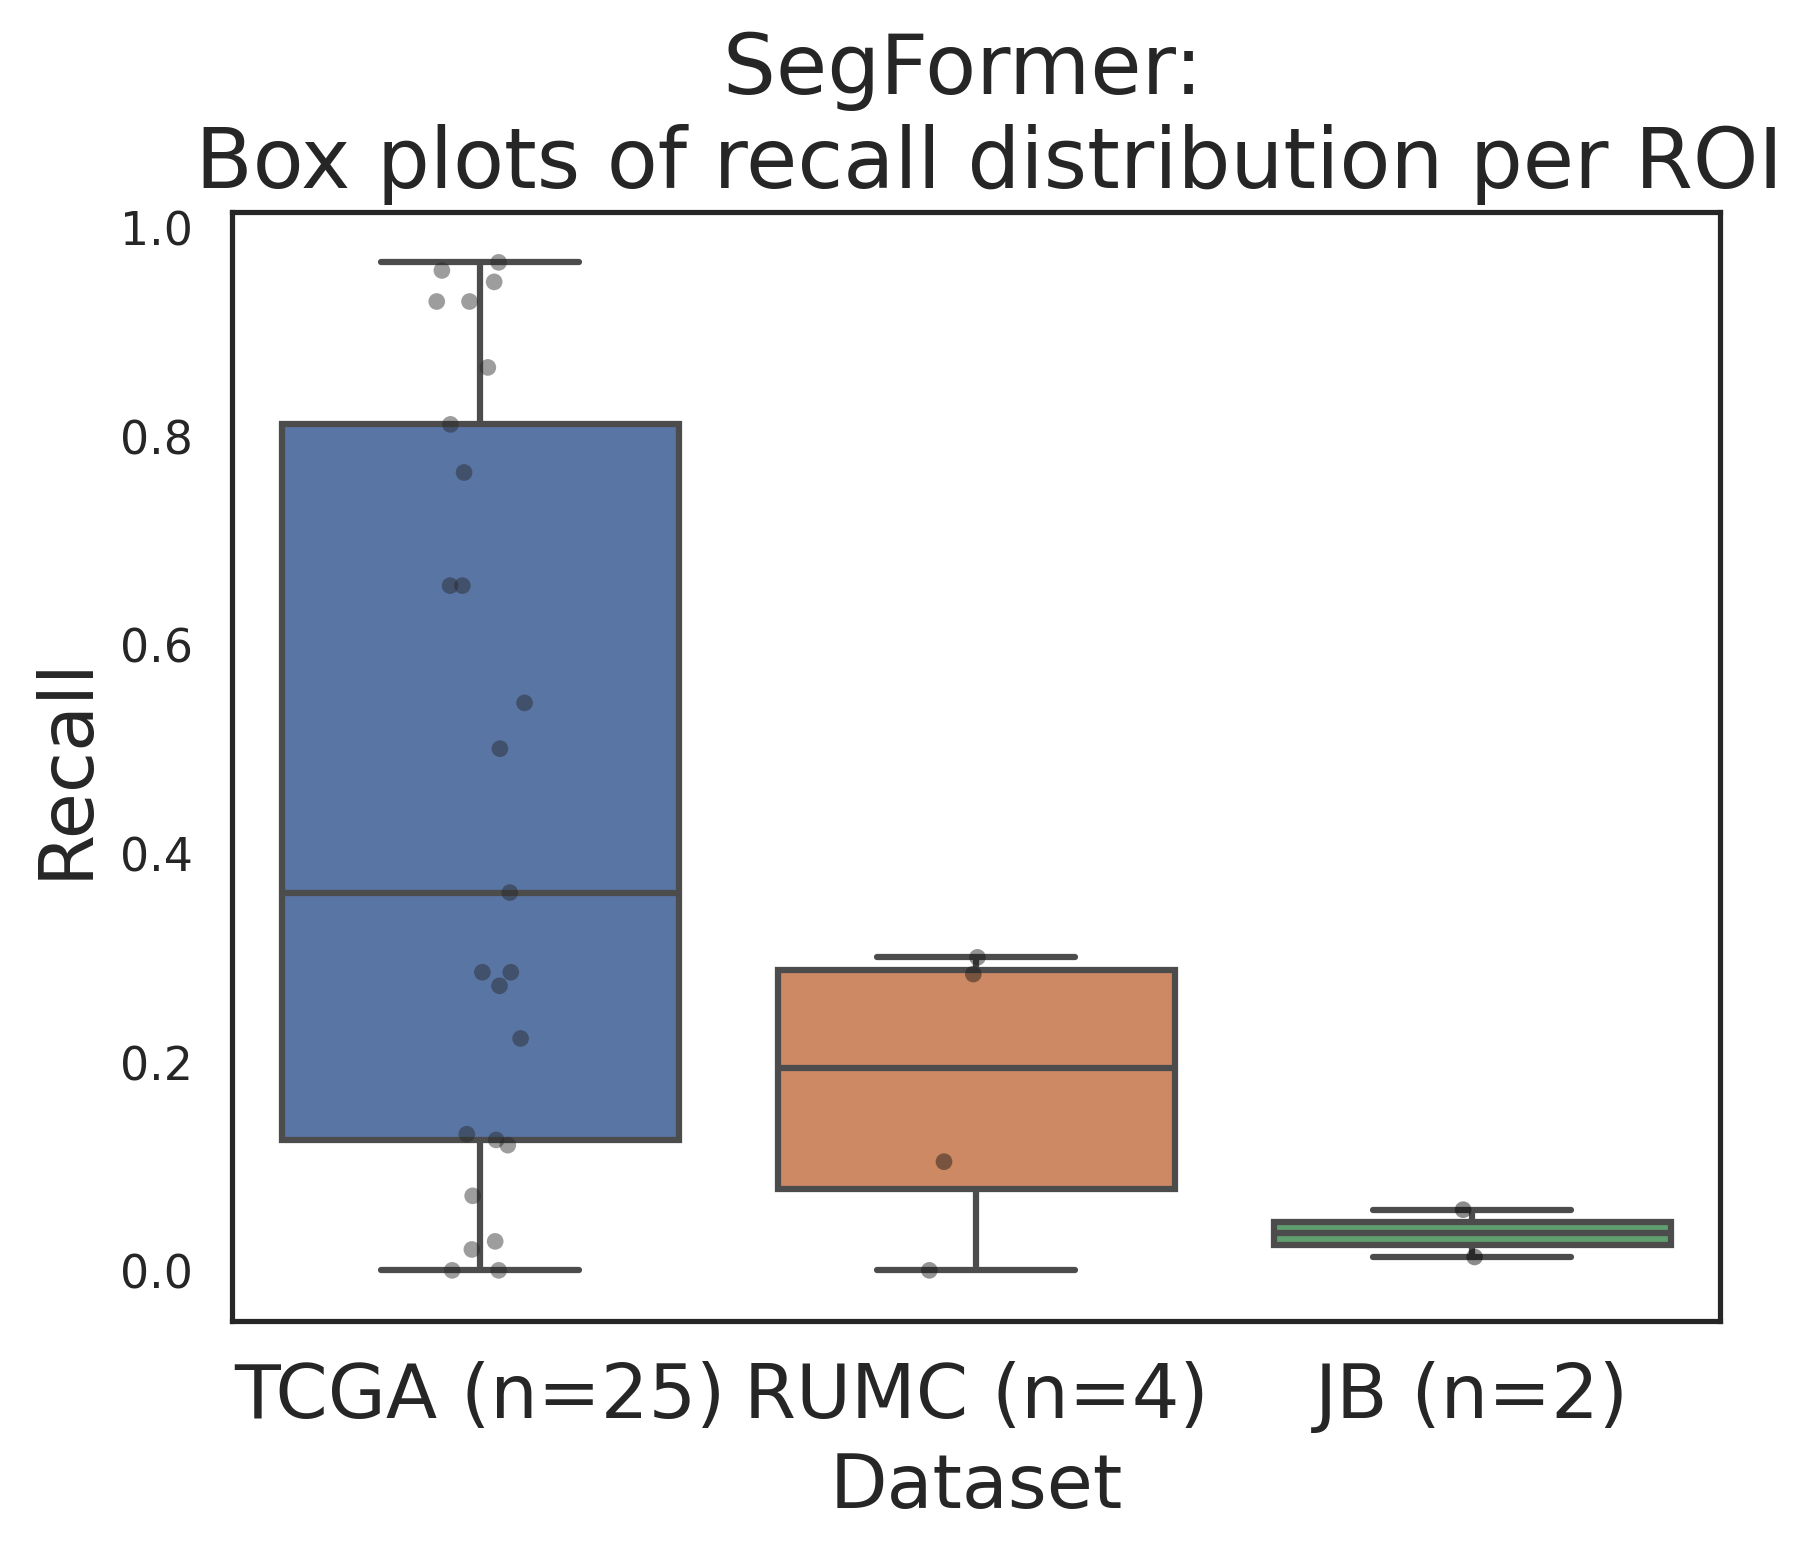
\includegraphics[width=.32\linewidth]{figures/tils/segformer_recall_roi_adj.png}
    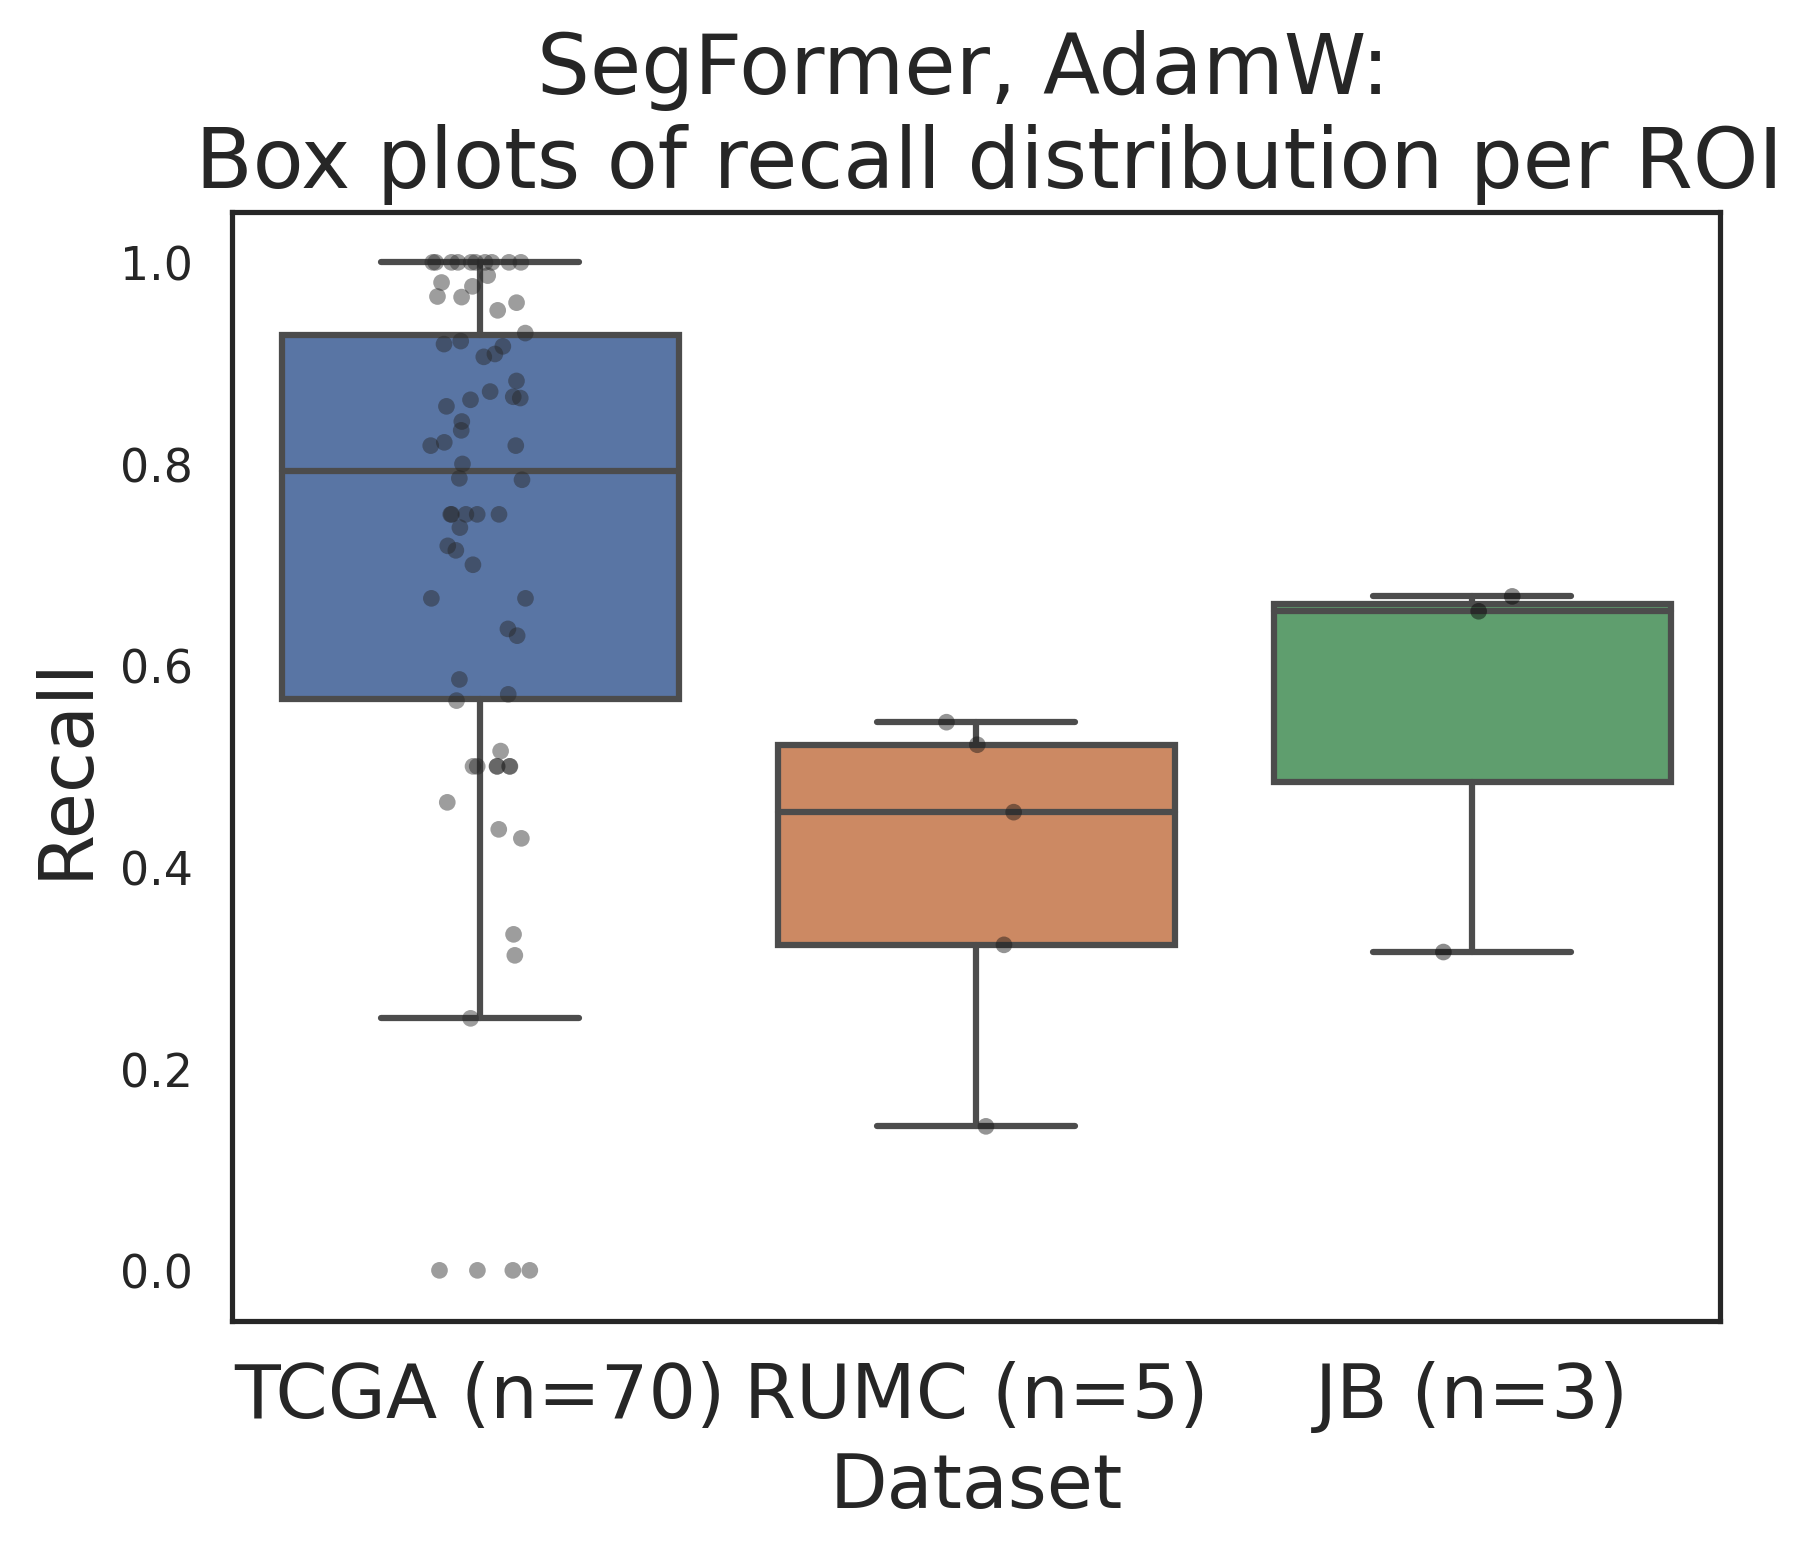
\includegraphics[width=.32\linewidth]{figures/tils/segformer,_adamw_recall_roi_adj.png}
    \caption{Boxplots of precision and recall across three datastes (TCGA-BRCA, RUMC, JB) with
    maximum allowed distance between ground truth and prediction equals 10 pixels (5 \textmu m).}
    \label{fig:tils_pr_r_boxplots}
\end{figure}

For model inference, the model with the best pixel-wise Dice score on the validation set was used.
Patches of size 128$×\times$128 were extracted from the tissue region at 20$\times$ magnification
with a stride of 100. The whitespace was extracted by using thresholding and
inference of non-background pixels was then performed.

\begin{figure}[H]
    \centering
    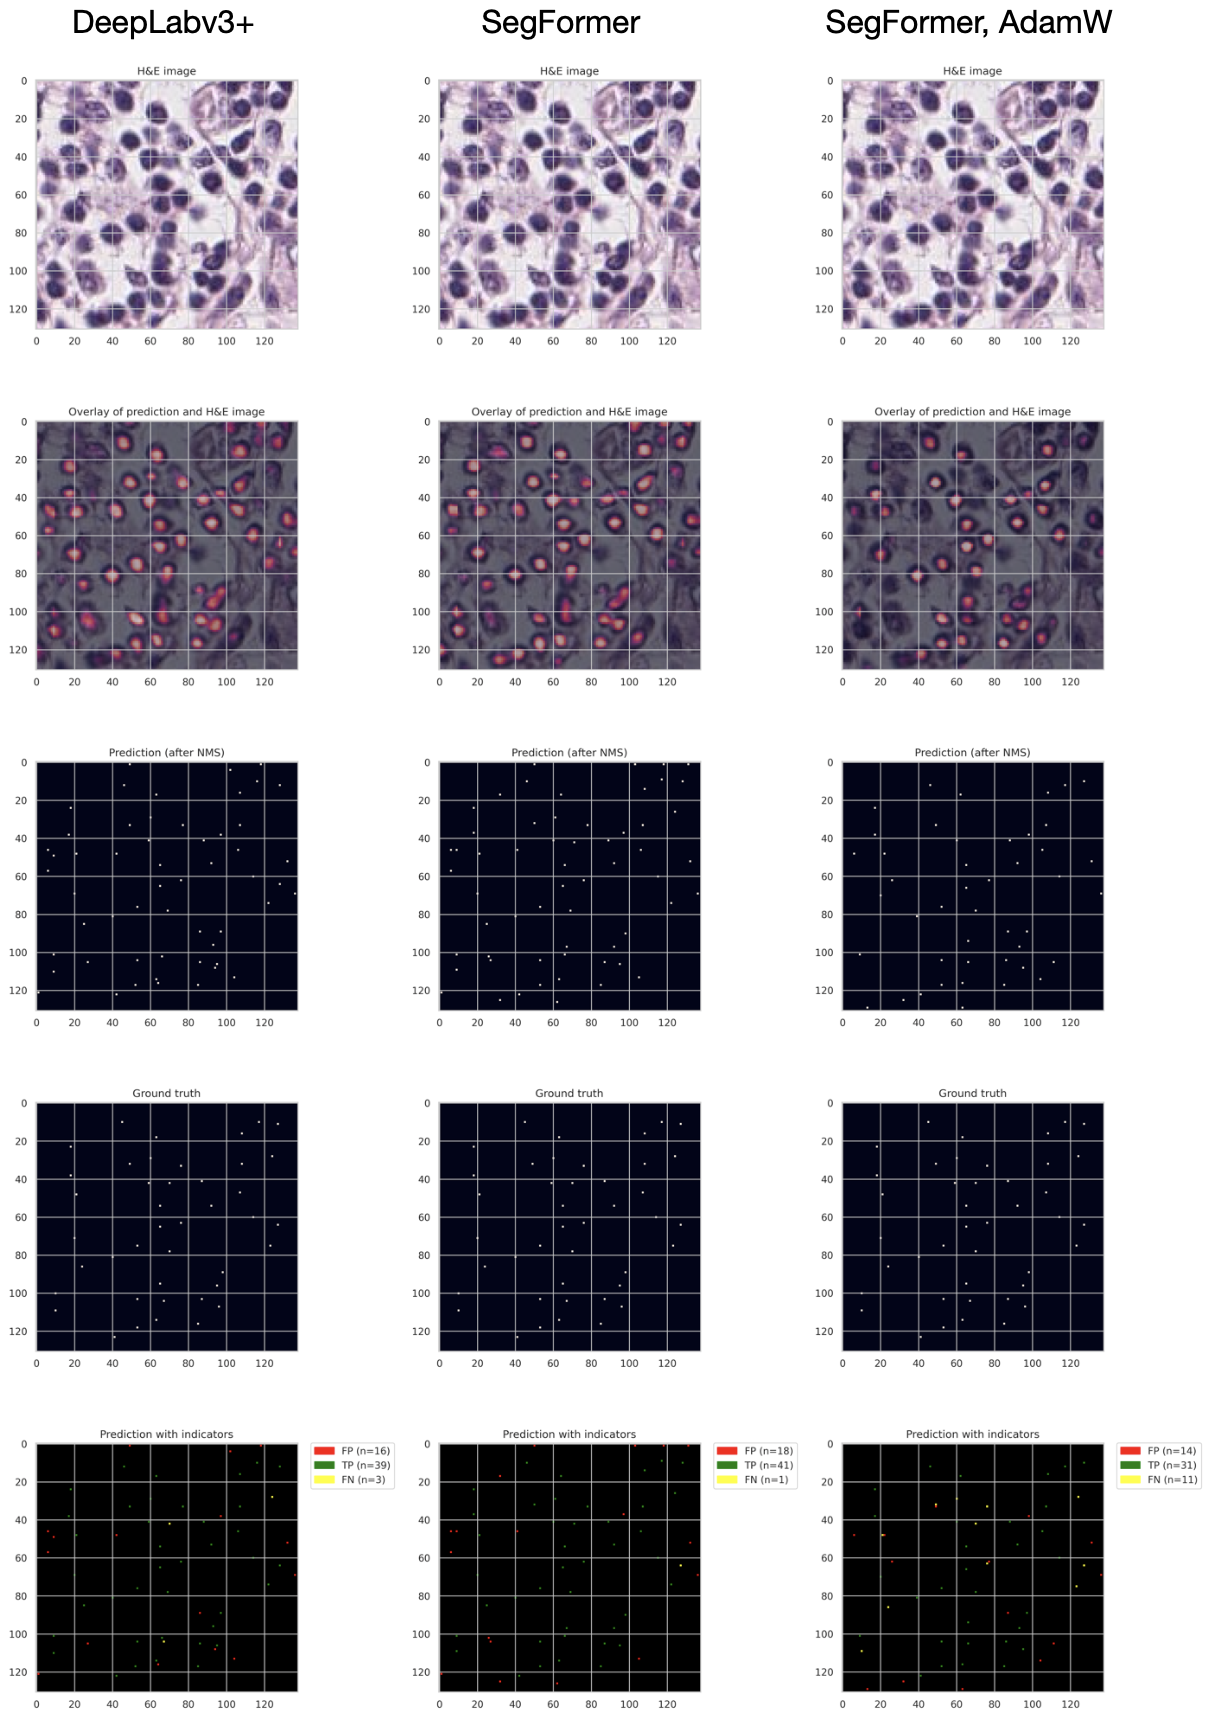
\includegraphics[width=0.95\textwidth]{figures/tils/TCGA-D8-A142-01Z-00-DX12.png}
    \caption{TCGA-D8-A142-01Z-00-DX12 TILs prediction with DeepLabv3+, SegFormer and
    SegFormer, AdamW. With 0.713, 0.804 and 0.812 F1 scores accordingly.}
    \label{fig:TCGA-D8-A142_tils}
\end{figure}

\section{Survival Analysis}
\todo[inline]{The following results are generated with DeepLabv3+ TILs detection. Missing heterogeneity features. Waiting for the results to generate. If everything goes wrong, those are the final results. Hopefully not.}
The patients from TCGA-BRCA clinical data with negative or not complete event times were removed. The remaining
1005 patients were used for survival analysis.
1133 segmented diagnostic slides were saved at 5$\times$ magnification. Each slide has determined regions of tumor, stroma,
and rest, as well as a list of all selected TILs. Based on this information four groups of TILs
densities were calculated: in stroma, stroma border, tumor associated stroma border,
and tumor border. The description of the regions is visualized in Figure~\ref*{fig:borders}.
The features for patients with multiple slides were mean aggregated.
\begin{wrapfigure}{r}{0.45\textwidth}
    \centering
    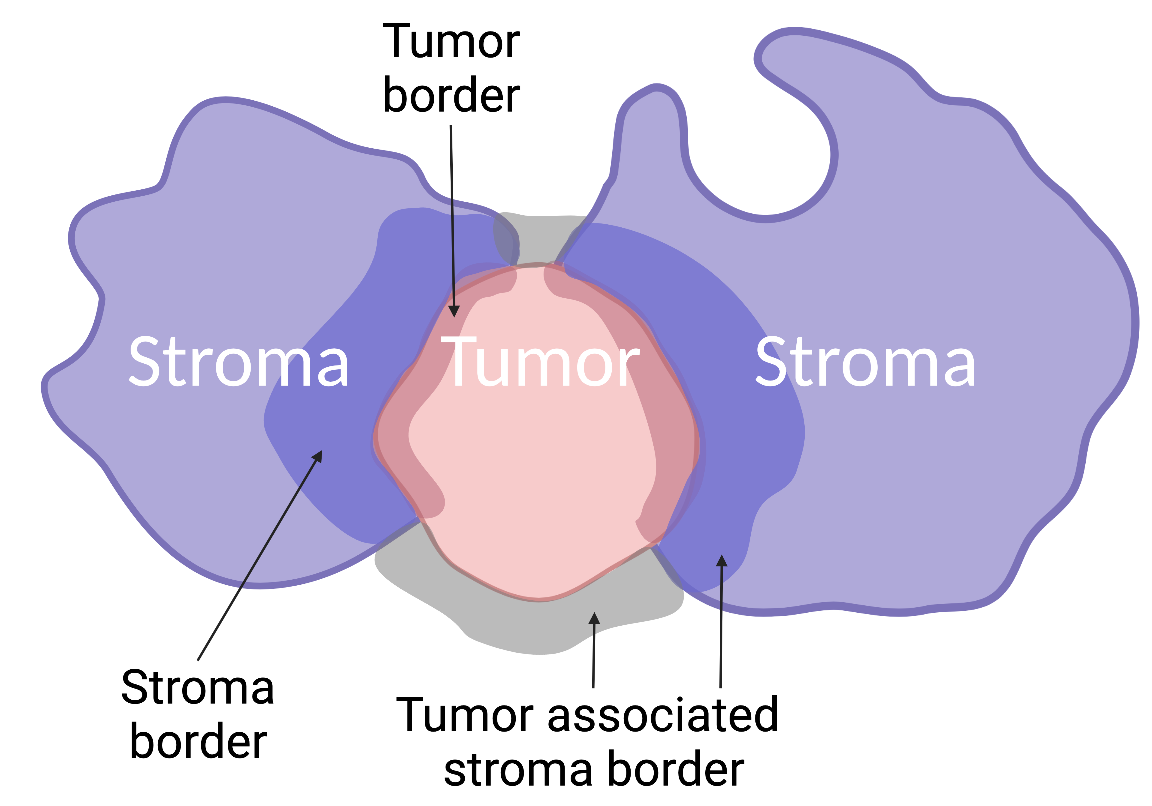
\includegraphics[width=0.45\textwidth]{figures/survival/tils_scheme.png} 
    \caption{Schematic border explanation. Created with BioRender.com}
    \label{fig:borders} 
\end{wrapfigure}
The overall TILs density in stroma was considered a baseline feature.
All densities were calculated as $\frac{\textrm{ Number of TILs}}{\textrm{Area in } mm^2}$.
For each border region, different widths were used. Tumor border experiments included
lower border widths of 10-40 \textmu m. Whereas stroma borders ranged between 50
and 350\textmu m.
Additionally, tumor associated stroma border of 125 \textmu m was included, since this is
the optimal border found for breast cancer patients~\cite{thagaard2021automated}.
It resulted in 20 features
that were first evaluated on correlation as depicted on a heatmap Figure~\ref{fig:heatmaps_tils}.
There are three coherent groups visible in Figure~\ref{fig:heatmaps_tils}.
There is a clear link between different groups and the baseline, such as a high correlation
of TILs density in stroma with TILs densities in stroma borders, which increases the bigger
the border gets. And on a contrary, a lower correlation of baseline with TILs density in tumor borders.
The values of pair-wise Pearson correlations in each group were compared and the columns with
a correlation higher than 90\% were removed. If all columns in a group displayed a
correlation above 90\%, the most similar column of a group was kept, which should
represent a group best. The resulting features and their correlations can be seen on the right heatmap
in Figure~\ref{fig:heatmaps_tils}.
\begin{figure}[h!]
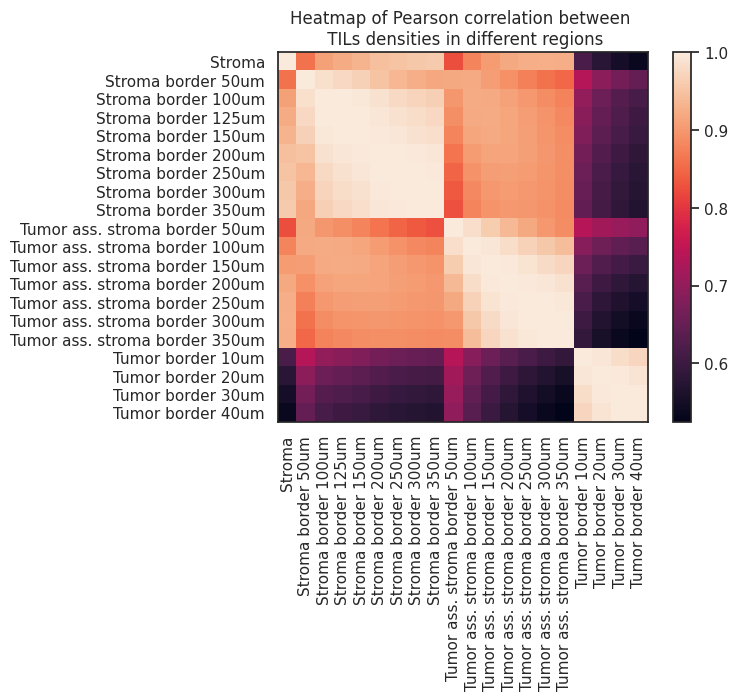
\includegraphics[width=.5\linewidth]{figures/survival/heatmap_tils.png}
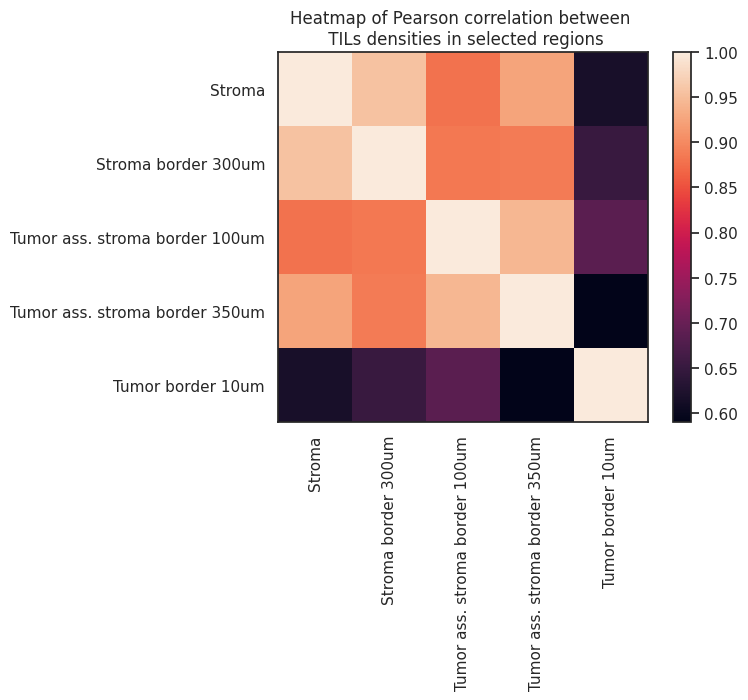
\includegraphics[width=.5\linewidth]{figures/survival/heatmap_tils_min.png}
\caption{Heatmaps representing pair-wise Pearson correlation between TILs densities in different areas.
Full version and condensed to group representatives.}
\label{fig:heatmaps_tils}
\end{figure}
For further comparison, features were evaluated at different prevalences.
For every feature, the patients were sorted descending according to a current feature.
For every prevalence in the range of 0.2 until 0.9, the patients were separated into
according groups and the Kaplan Meier method was used on both of them. The Log-Rank test
was applied to measure whether the two resulting event series are statistically different.
The resulting p-values are visualized in Figure~\ref{fig:pvalues_tils}, both as a line plot
per each prevalence, as well as a boxplot. In the boxplot, it can be seen that the median
p-value of the density in 100 \textmu m tumor associated stroma and in 10 \textmu m tumor
border lay higher than the other features. Those densities are also found more frequently
over the statistical significance line in the line plot. Those features were decided to exclude.
And for visibility, the remaining features were plotted again separately in
Figure~\ref{fig:pvalues_tils_selected} with an additional boxplot depicting differences in median
survival time at the same prevalence range. TILs density in tumor associated stroma achieving
lower p-values in the lower prevalences. But TILs density in stroma border shows a better
performance overall. It is also a feature that stays under the significance line across
all prevalences. Additionally, according to the Median survival time boxplot,
the median value of TILs densities in stroma border is 1.5 years higher.

For fitting the data into a Cox model, the TILs densities were divided by 100.
The result revealed 0.58 concordance, 0.01 p-value, and 0.94 hazard ratio.
That means that the coefficient is negative (-0.06) which supports the assumption
that the high level of TILs plays a role in longer survival probability.
For the TILs density in stroma border, the result is identical: 0.58 concordance,
0.01 p-value, and 0.94 hazard ratio. And TILs density in tumor associated stroma
reaches 0.59 concordance, 0.01 p-value, and 0.88 hazard ratio.
Regression models generally give more reliable results with normally-distributed variables.
Since the TILs densities are not normally-distributed (see Figure~\ref{fig:histo_tils}),
the experiments were repeated with log features. The TILs densities in stroma scored
0.58 concordance, p-value 0.00064 and 0.8 hazard ratio, for TILs desnities in stroma border - 0.58
concordance, p-value 0.00034 and 0.79 hazard ratio, and TILs densities in tumor
associated stroma - concordance of 0.59, p-value 0.00019 and 0.78 hazard ratio.
It was expected for concordance to stay indifferent since it was not influenced by
taking the log of all values. Whereas p-values and hazard ratios improved drastically.
It is harder to explain the signal presence and meaning of log-ed features,
hence we will concentrate on raw values.

\begin{figure}[H]
\centering
\includegraphics[width=0.4\linewidth]{figures/survival/histo_tils.png}
\includegraphics[width=0.4\linewidth]{figures/survival/histo_tils_log.png}
\caption{Histograms of baseline TILs density in stroma features versus its log distribution.}
\label{fig:histo_tils}
\end{figure}
    

The Kaplan Meier curves in Figure~\ref{fig:km} at most often viewed prevalences of
0.33, 0.66, and the median matched the cases when TILs density in tumor associated
stroma features stratified patients better in lower range and median.
Whereas at 0.66 the TILs density in stroma border scores a slightly more significant p-value.
The observation that a border of stroma or tumor associated stroma features perform better
than the stroma itself may come from the observed behavior that the tissue segmentation model
leans to confuse rest with stroma (Figure~\ref{fig:tissue_confusion}).
Hence, taking into consideration only regions close to tumorous regions, that are better
segmented, acts as a filtering of falsely annotated regions that therefore leads to a higher
significance of a feature.

\todo[inline]{When the final results are done, here same analysis of Her2+, TNBC subsets.}

\begin{figure}[h!]
\includegraphics[width=\linewidth]{figures/survival/pvalue_prevalence_all.png}
\includegraphics[width=0.764\linewidth]{figures/survival/pvalue_boxplot_all.png}
\caption{Log-Rank p-values distribution by different patient separations.
The dotted line in the line plot represents the significance level of 0.05 ($\log_{10} 0.05$)}
\label{fig:pvalues_tils}
\end{figure}

\begin{figure}[h!]
\includegraphics[width=\linewidth]{figures/survival/pvalue_prevalence_selected.png}
\includegraphics[width=0.5\linewidth]{figures/survival/pvalue_boxplot_selected.png}
\includegraphics[width=0.5\linewidth]{figures/survival/surv_time_boxplot_selected.png}
\caption{Log-Rank p-values distribution by different patient separations with an additional boxplot
with median survival time differences. The dotted line in the line plot represents the significance level of 0.05 ($\log_{10} 0.05$)}
\label{fig:pvalues_tils_selected}
\end{figure}

\begin{figure}[h!]
\includegraphics[width=\linewidth]{figures/survival/km_33.png}
\includegraphics[width=\linewidth]{figures/survival/km_50.png}
\includegraphics[width=\linewidth]{figures/survival/km_66.png}
\caption{Kaplan Meier curves. Columns correspond to denisty features in: stroma, 300 \textmu m stroma border,
100 \textmu m tumor associated stroma border. Rows coorespond to following prevalences: 0.33, 0.5, and 0.66.}
\label{fig:km}
\end{figure}

%\begin{figure}[h!]
%\includegraphics[width=0.5\linewidth]{figures/survival/boxplot_sep.png}
%\caption{Value separation}
%\label{fig:v_sep}
%\end{figure}
\chapter{Conclusion}
In this thesis, a new pipeline for TILs scoring in breast cancer patients was presented.
The tasks of tissue segmentation and TILs detection for WSI were approached with DeepLabv3+
which is actively used in computational pathology, as well as with a novel transformer-based
approach, SegFormer. As a result, the SegFormer was found to be superior in the TILs
segmentation task. The analysis of TCGA-BRCA slides with the resulting models, allowed
for experiments with different TILs density based features. Several of them showed the
ability to successfully stratify patients at multiple prevalences. This proves a strong
signal of TILs in the TCGA-BRCA dataset, which was not previously demonstrated while
analyzing exclusively this publically available dataset. 

As an outlook, one of the main missing prospects of this work is the absence of
benchmarking with the existing challenge entries. Due to the late start of this
work the submission portal was closed by the time the models were present. 
The TiGER challenge team that achieved the highest rank on the preliminary leaderboards
for both segmentation of tissue and TILs published their approach before the challenge ended.
The authors~\cite{shephard2022tiager} trained Efficient-UNet-B0 for both tasks using Jaccard loss.
The model was trained via a stratified 5-fold
cross-validation framework with 512$\times$512 patches at 10$\times$ magnification,
with a stride of 256 pixels. Whereas for TILs segmentation,
the patches of 128$\times$128 were extracted at 20$\times$ magnification, with a stride of 100 pixels.
The selected model with the best F1-score across each experiment on 5-fold cross-validation achieved
a dice score of 0.762 for tumor segmentation, 0.718 for stroma segmentation, and  0.702 for TILs
detection. The TILs score was calculated by dividing the total predicted TILs area by the stromal
area and multiplying by 100. The score was further constrained to be an integer between 0 and 100.
The resulting TILs scores got the highest concordance of 0.719 for predicting survival as part of
a Cox proportional hazards model. Right now any of the results in this paper or any future papers
of the TiGER challenge can be compared to the results in this thesis. Due to the arrangement of the
challenge, the reported results are based on hidden test set and internal clincal data.
As long as the submission server is closed, those models and ideas need to be reimplemented.
Besides benchmarking, those challenge entries can provide valuable ideas for improvements to the current pipeline.
Such as applying transfer-learning, by using this model with pre-trained weights from ImageNet for tissue
segmentation or an on-the-fly under-sampling approach to alleviate class imbalance of TILs segmentation task.
There are also some parallels in approaches such as, similarly to this thesis, the authors~\cite{shephard2022tiager}
viewed TILs detection problem as TILs segmentation, but additionally, applied stain augmentation. Even though the
importance of the stain addition could be
suspected from the tissue segmentation results, this is a valuable experiment that should be performed.
All in all, this thesis also provides a better understanding and test possibilities for TILs features development.
Instead of blindly submitting a value, adapting the TCGA-BRCA data set enables it to actually view the data specifics
which could have helped the participants of the challenge (applicable if of course TCGA-BRCA data is not included in
the hidden clinical data).

%\appendix{}

% TODO: appendix chapter
%\chapter{General Addenda}

If there are several additions you want to add, but they do not fit into the thesis itself, they belong here.

\section{Detailed Addition}

Even sections are possible, but usually only used for several elements in, e.g.\ tables, images, etc.
\chapter{Appendix}
\begin{figure}
\includegraphics[width=\linewidth]{figures/tissue/dices_patients.png}
\caption{EXAMPLES for TILs prediction models. A lot of test comming up here.}
\label{fig:figure3}
\end{figure}

\begin{figure}
\includegraphics[width=.5\linewidth]{figures/tissue/deeplabv3+_prec_patient_wsirois.png}
\includegraphics[width=.5\linewidth]{figures/tissue/deeplabv3+_recall_patient_wsirois.png}

\includegraphics[width=.5\linewidth]{figures/tissue/segformer_prec_patient_wsirois.png}
\includegraphics[width=.5\linewidth]{figures/tissue/segformer_recall_patient_wsirois.png}

\includegraphics[width=.5\linewidth]{figures/tissue/segformer,_adamw_prec_patient_wsirois.png}
\includegraphics[width=.5\linewidth]{figures/tissue/segformer,_adamw_recall_patient_wsirois.png}

\caption{EXAMPLES for TILs prediction models. A lot of test comming up here.}
\label{fig:figure3}
\end{figure}

\chapter{Figures}
\section{Example 1}
\cmark
\section{Example 2}
\xmark

\microtypesetup{protrusion=false}
\listoffigures{}
\listoftables{}
\microtypesetup{protrusion=true}
\printglossaries
\printbibliography{}

\end{document}